
{\chapter{Exploring the single-cell RNAseq analysis landscape in timeseries patient derived xenografts 
\\
\textit{(Manuscript in preparation)}}}

 \label{ch:Chapter5}


 \section{Motivation}

%\printinunitsof{in}\prntlen{\textwidth}
%\printinunitsof{in}\prntlen{\textheight}
% The text width is 6.5in -- important for plotting
% The text height is 9in

To further enhance understanding of how fitness under drug treatment occurs, I sought to identify genomic and non-genomic basis for transcriptome differences. 
In TNBC, copy number changes have a major influence on the expression landscape \cite{wang2016integrative}.
Although many studies have analyzed CNV and differential gene expression of distinct oncogenes and tumour suppressor genes in various cancers \cite{kuzyk2015mycn, budczies2016pan, kwak2015fibroblast}, to date there has been no precise study that explores the relationship between CNV and differential gene expression and clonal drug resistance,  across multiple tumour samples at single cell level. It is unclear to what extent the expression level is affected by CNV at single cell level.
In Chapter 4, a system for identifying copy number defined clones was established and here, I intend to exploit that information to obtain scRNA-seq clones by mapping 10x scRNA-seq with \texttt{clonealign} to CNA genotypes \cite{campbell2019clonealign}.

Since \ac{DLP+} allows identification of regions of the genome that differ between the clones and the regions that are similar \cite{laks2019clonal}, therefore, I would be able to define which regions of the transcriptome might be influenced by CNA driven expression and those that might be independent of change in copy number state.

Because of the difficulty to analyse longitudinal patient samples for single cell gene expression and the lack of multiple longitudinal pre-clinical breast cancer models, these questions remain unexplored and our understanding of how they relate to TNBC heterogeneity is limited.

Here, I aimed to systematically investigate the specific relationship between copy number change and differential gene expression across timeseries TNBC PDX for which I have clonal copy number proportions already analysed in Chapter 4. 

%In spite of advanced technologies and treatment, triple negative breast cancer still faces the problems of tumour recurrence and drug resistance.
%For any given difference between the types of drug resistance, for example the expression of a particular gene, it is assumed that differences arise deterministically or probabilistically in the presence of transcription factors regulating the genes in the tumours. Cancer cells in distinct cell states often exhibit important differences in functional properties depending on which genes are turned on and off resulting in sensitive or resistant phenotypes.

%The most challenging analysis is to differentiate whether the change in gene expression leading to change in cellular state is stochastic \cite{raj2008nature} or deterministic to produce the same output under similar environment.
%Previously it was shown that unique cells within a population can exhibit fluctuations in gene expression that could predict distinct phenotypes \cite{shaffer2019memory}.

%I set to explore 3 timeseries breast cancer patient derived xenografts (PDX) that were serially challenged for around 4-5 cycles with one or two drugs until and beyond they started showing resistant behaviour. The aim is to measure the magnitude of fluctuations in gene expression from sensitive to resistant phenotype.
%This study may help us better understand the correlation between CNV and differential gene expression and provide new insights into the mechanism of development and progression of cancers with potential biomarkers in triple negative breast cancer.

 \section{Synopsis}





%The overall goal of this chapter is to determine the impact of change in copy number on gene expression. By using single cell RNA sequencing in conjunction with \texttt{clonealign}  \cite{campbell2019clonealign}, a proportion of the genome  was defined that was affected by copy number dependent transcription.
 
 %This chapter is divided into 3 sections of data evaluation, copy number dependent transcriptome proportions and change in gene expression over time. Highlights in synopsis are followed by detailed results: 
  
  \subsection{ScRNA-seq data processing and evaluations for downstream analyses} 
\begin{itemize}
  
   \item Generated scRNA-seq data for 145,858 single cells across 3 TNBC timeseries PDX 
(TNBC-SA609, TNBC-SA1035, TNBC-SA535) that were serially challenged for 4-5 cycles of (cisplatin) platinum and SA535 additionally with CX5461 to create resistance.
   \item I performed  \texttt{edgeR} and \texttt{SCTransform}  normalization which resulted in similar distributions of post-normalized expression in all 3 timeseries data. TNBC-SA609 showed the highest correlation coefficient of 0.94 among all 4 timeseries.
 
 \item Normalization with \texttt{SCTransform} partially removed batch effects with a small range of mean gene expression differences.

 \item scRNA-seq with \texttt{clonealign} assignments to CNA clones were strongly correlated.
 
 \item Clone copy number structure was visible in dimensional reduction (UMAP), indicating CNA-clone specific gene expression could be identified, although some residual batch effect was also noticeable.

\end{itemize}
\subsection{Contrasts of resistant and sensitive clone specific gene 
expression reveals the rates of \textit{in cis} and \textit{in trans} components} 
\begin{itemize}
   
   \item Copy number change \textit{in cis} expression accounts for $\sim${6.3\%-38.52\%} of clonal differences in resistant vs sensitive transcriptomes. 
   %The overall number of \textit{in trans} genes were higher as compared to \textit{in cis}, which was consistent with previously reported results.
 
 
 %\item For all DE comparisons, DE in-cis genes average was 38.52\% (sd=11.43) for SA609, SA535 cisplatin, SA535 CX5461,  however, the proportion of DE in-cis genes for SA1035: average was 6.3\% (sd= 0.92).
 
 
 \item  In 4 published cancer fitness and cisplatin resistance datasets, differentially expressed (DE) genes showed highest match \textit{in cis} for TNBC-SA535, in both treatment regimes with 28\% maximum followed by TNBC-SA609 with 12.8\%. In contrast, TNBC-1035 had the lowest \textit{in cis} DE match with only 2.4\%.

 \item Average \textit{in cis} calculated proportion of gene set membership of  4 reference gene sets were 10.3\%, 10.44\%, 12.8\% for SA609, SA535:cisplatin, SA535:CX5461, respectively. On the other hand, \textit{in trans} average proportions were 16.8\%, 14.02\%, 15\% for SA609, SA535:cisplatin, SA535:CX5461, respectively. However, SA1035 being unique, had average proportions of 1.07\% \textit{in cis} and 22.4\% \textit{in trans}.

 \item Overall, in all DE \textit{in cis} regulated genes, the highest average of positive linear up or down regulation with copy number was found in TNBC-SA1035 with average of 88.3\% (sd=3.9) and lowest in TNBC-SA609 with average of 74.1\% (sd=13.2). 
 TNBC-SA535:Cisplatin, SA535-CX5461 showed 83.7\% (sd=6.5) and  85.7\% (sd=3), respectively.
 
 \item Cisplatin resistance associated genes regulated both \textit{in cis} and \textit{in trans} were observed in the extremes of the distribution of differentially expressed genes, such as,
 
 \textbf{\textit{in cis}} regulated included \textbf{COX6C}: \textbf{Oxidation phosphorylation pathway}, pre-target cisplatin resistance; \textbf{ID1}: \textbf{TGF beta pathway}, pre-target cisplatin resistance; \textbf{HSPs}: \textbf{Hypoxia pathway} (Off-target cisplatin resistance);  \textbf{TMEM45A}: \textbf{Hypoxia pathway} (post-target through pro-apoptotic effects and also off-target cisplatin resistance); \textbf{ID4}: \textbf{Hypoxia pathway} (Off-target cisplatin resistance).  
  %\textbf{PI3}: , TMEM45A

   \textbf{\textit{in trans}} regulated included  \textbf{UQCRB}: \textbf{Oxidation phosphorylation pathway} (pre-target cisplatin) resistance;  \textbf{CRABP1} (post-target cisplatin resistance); \textbf{NDUF: Oxidation phosphorylation pathway} (pre-target cisplatin resistance). 
 %textbf{ATP5MPL}:  CXCL3, S100P, S100A7, HERC5, IFITM3, NDUF and

 \item Importantly, the average \textbf{CNA mediated platinum resistance} accounts for, from highest to lowest proportion: SA535:CX5461: 7.47\% (sd=3.69); 
SA609: 6.6\% (sd=3.47); SA535:Cisplatin: 5.8\% (sd=4.73)
SA1035:0.52\% (sd=0.6). 
 
  \item Commonly upregulated pathways in 3 TNBCs-SA609, SA535:Cisplatin and SA535:CX5461 included \textbf{TNF} (post-target/off-target cisplatin resistance), EMT (on target/post-target cisplatin resistance) \textbf{TGF  beta  signaling},  \textbf{HYPOXIA} (post-target through pro-apoptotic effects and also off-target cisplatin resistance), \textbf{APOPTOSIS} (post-target through pro-apoptotic effects and also off-target cisplatin resistance), \textbf{E2F} (On-target cisplatin resistance), \textbf{MITOTIC SPINDLE and ESTROGEN  RESPONSE}, whereas \textbf{OXPHOS} (pre-target cisplatin) was downregulated. 
 
 \item \textbf{OXPHOS} (pre-target cisplatin) and \textbf{INTERFERON pathways} (Off-target cisplatin), were only upregulated in TNBC-SA1035.
 
 \item Cisplatin and CX5461 treated SA535 shared 13 upregulated pathways, with $\sim$ 20\% and $\sim$ 40\% \textit{in cis} regulation and $\sim$ 80\% and $\sim$ 60\% \textit{in trans} regulation of DE, respectively. Only one pathway, namely \textbf{Oxidative phosphorylation (OXPHOS)}, was down regulated in both series, suggesting their specificity to the tumour.

\end{itemize}

\subsection{Change in gene expression over time}

\begin{itemize}
 
  \item Line trajectories of individual genes over time showed that expression change could be monotonically increasing or decreasing under drug selection, for example, \textit{in cis} regulated \textbf{VDAC3  (OXPHOS pathways)} and \textit{in trans} regulated, \textbf{BTG1 (TNFA via NFKB pathway)}. 
 
   \item Similarly, in SA1035, \textit{in cis} regulated \textbf{UQCRB, from OXPHOS pathways} and \textit{in trans} regulated \textbf{TXN from Glycolysis} were found to be increasing with drug over time
 
 \item In some of drug holiday samples, when drug pressure is kept off, I observed a shift of expression towards untreated side, for example, drug holiday samples of SA1035 \textit{in cis} regulated \textbf{UQCRB (OXPHOS pathway)}, and drug holidays samples of SA609 \textit{in trans} regulated, \textbf{MYC (MYC targets V2)}.

 
 \item Most of the chemoresistance associated pathways were activated in the later passages with repeated exposure to drugs.
 

 %\item In TNBC-SA535, common precursor clone R, in comparison with untreated sensitive clone, showed additional upregulation of HEDGEHOG and ANDROGEN RESPONSE pathways in TNBC-SA535.

 \item Pathways analysis overtime showed a gradual increase in pathway representation, such as \textbf{MYC targets V1 and V2 in SA609, EMT and E2F targets}. All last time points had a greater number of significant pathways and there was a strong representation of known cisplatin resistance pathways, such as \textbf{TNFA, EMT, signaling via NF-$\kappa$B, TGF  beta  signaling, MTORC1, IL-2\_STAT5 signaling, KRAS signaling down, Hypoxia and Apoptosis}. 

 \item Gene expression changes over time highlighted activation of EMT, metabolic and cisplatin resistance pathways with repeated exposure of drugs.


 \item The common lineage precursor of two resistant clones, \textbf{clone R}, predominantly showed upregulation  of \textbf{EMT, KRAS, TNFA signaling via NF-$\kappa$B and Apoptosis pathways} as compared to untreated fit but drug sensitive \textbf{clone J}.
 
  \item Cisplatin and CX5461 treatment shared many pathways that showed time dependent dynamics in SA535, such as \textbf{TNFA signaling via NF-$\kappa$B, Hypoxia, Apoptosis, UV response up, KRAS signaling up, Inflammatory response, Epithelial mesenchymal transition, TGF Beta signaling, Estrogen response} and \textbf{p53 pathways.}

\end{itemize}

\begin{figure}
\centering
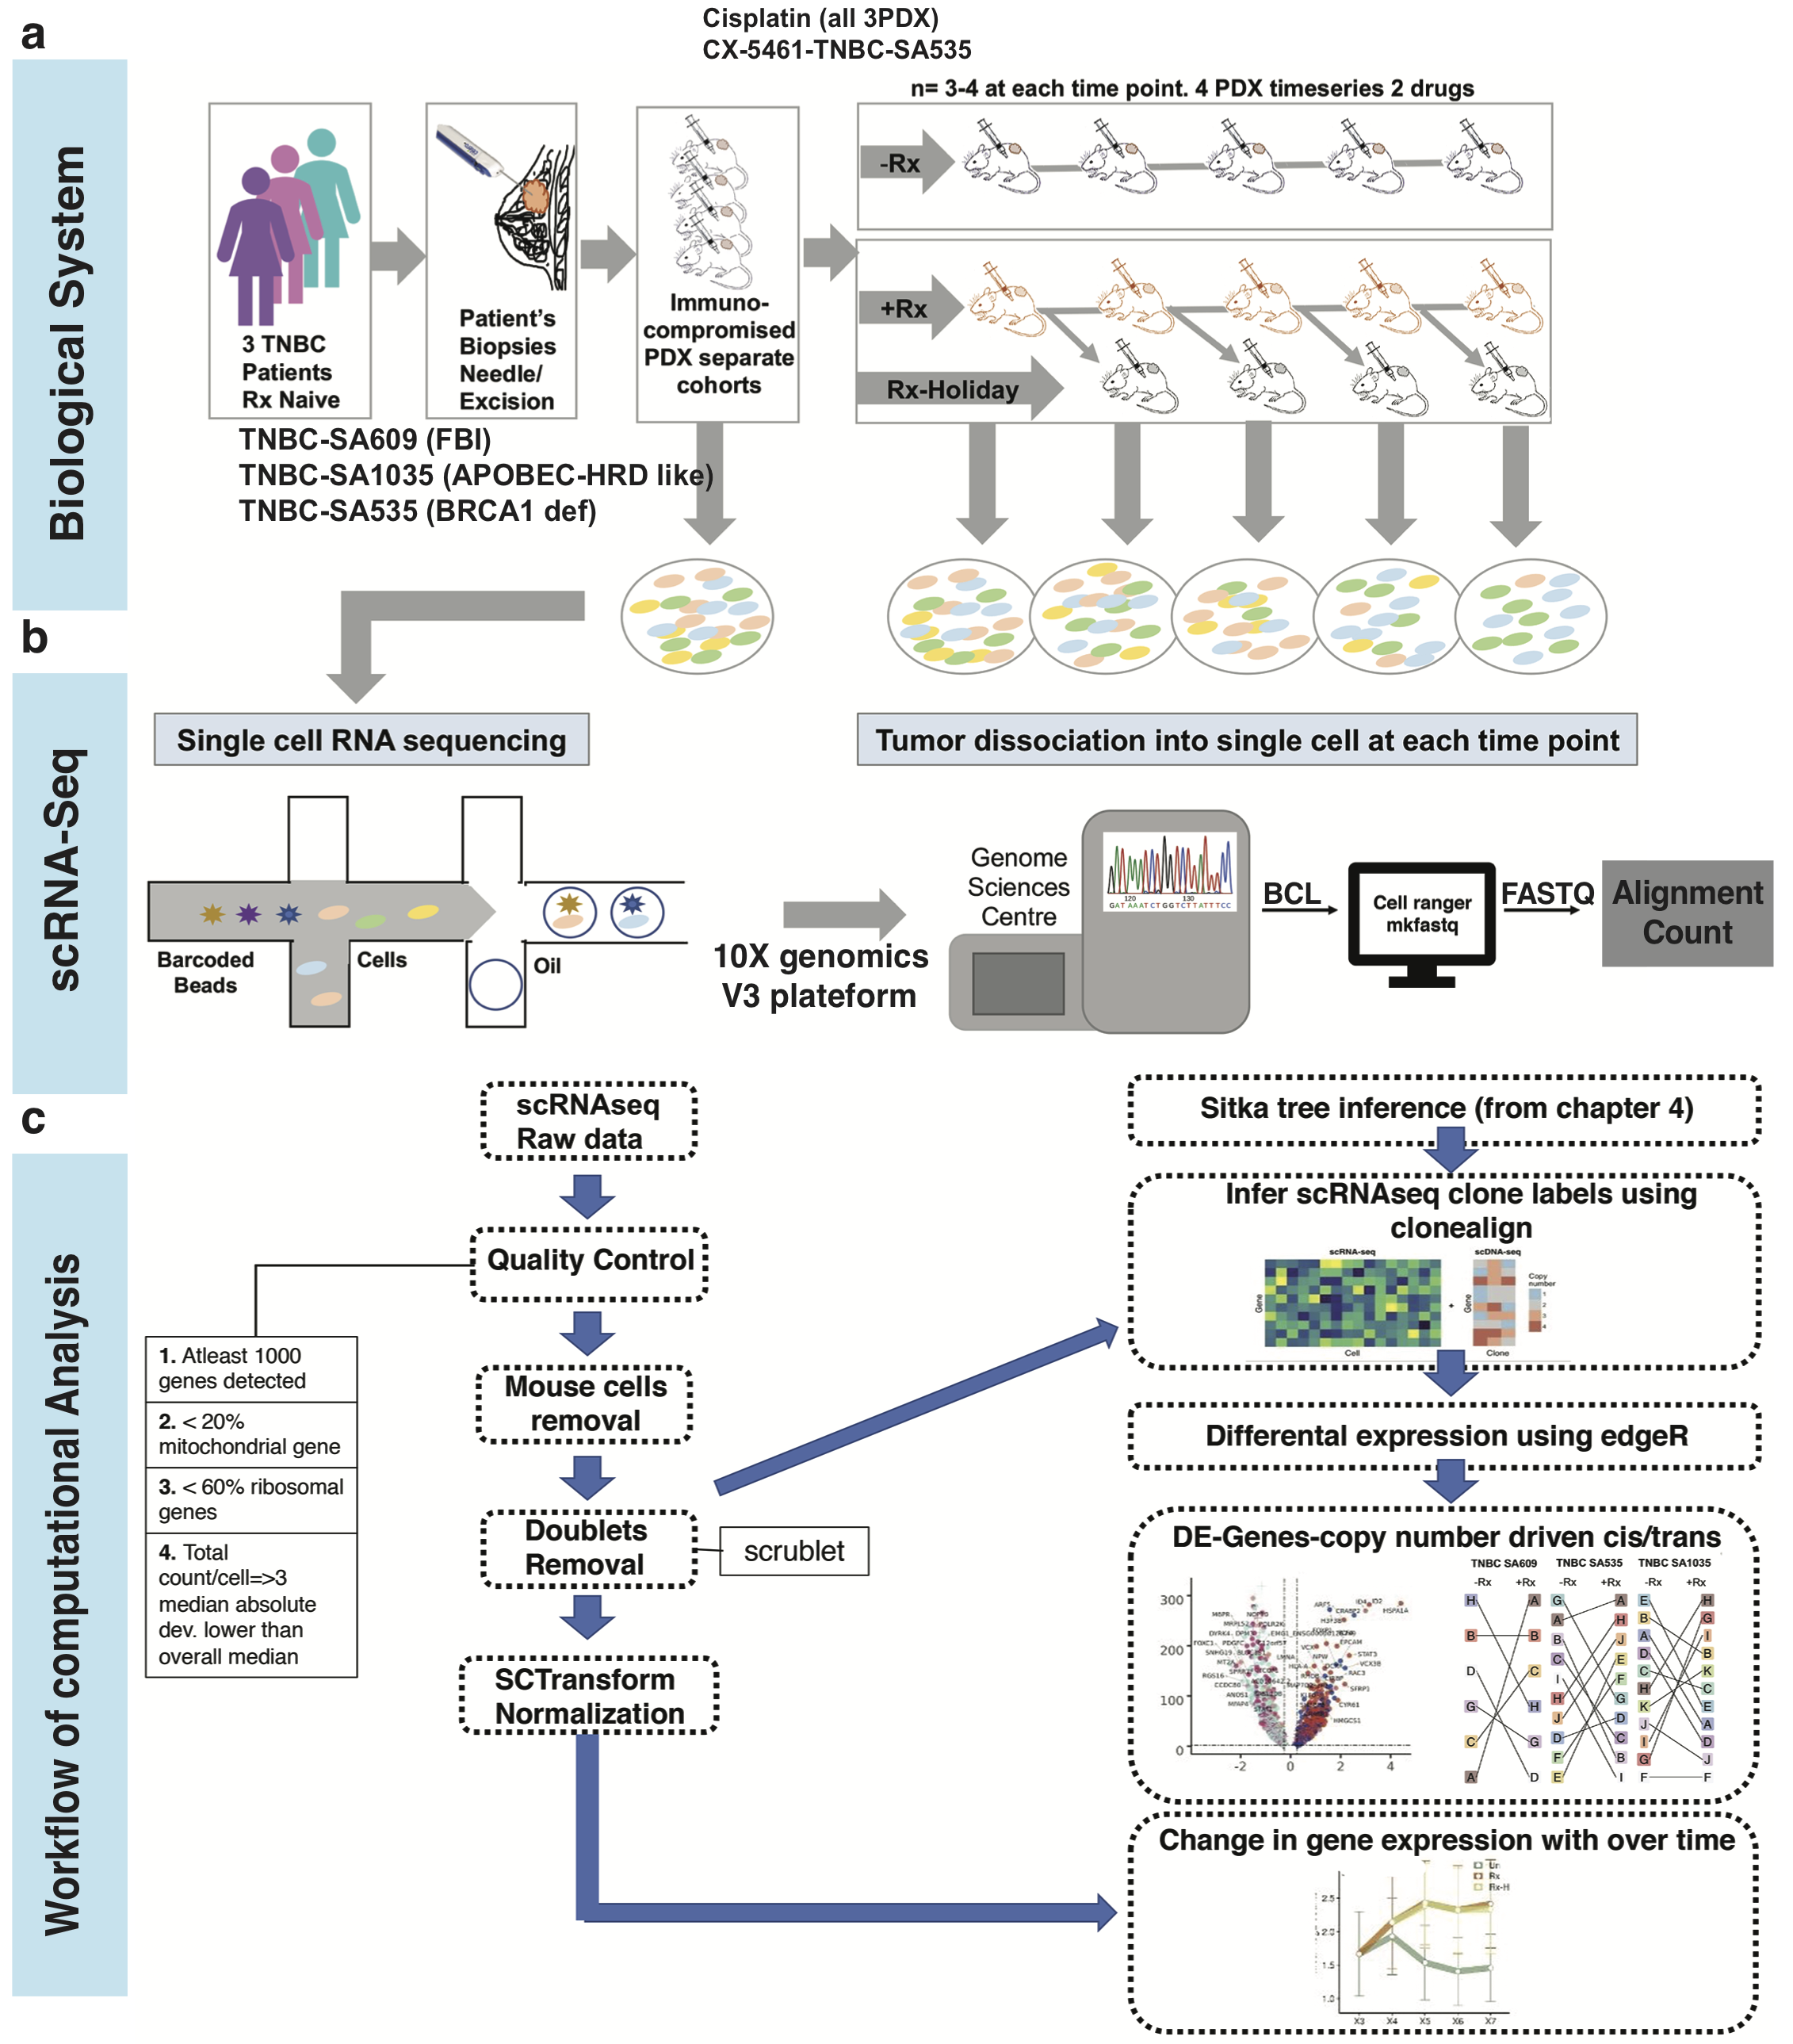
\includegraphics[width=\textwidth]{Figures/chap5/RNAworkflow.png}
	
\caption[Schematics of experimental design and analysis workflow]
	{\small
	\textbf{Schematics of data generation and analysis workflow.}
	   \textbf{(a)} Overview of the experimental design same series as of Chapter 4.
	    \textbf{(b)} Single cells RNA library prep. and sequencing.
	    \textbf{(c)} Computational workflow analysis used in this chapter.
	}
	\label{fig:chap5RNAworkflow}
\end{figure}
%------------------------------------------------------------------------------
\newpage

\section{Results}
 
%\subsection{Longitudinal single-cell RNA sequencing of patient-derived xenografts}
\subsection{Data collection and processing sets the ground for biological analyses} 
  
\subsubsection{Sample collection and workflow of data generation and analysis from triple negative breast cancer timeseries PDX}
To understand resistance at the scRNA-seq level, I selected 4 PDX timeseries that were developed by transplanting patient's tumour biopsies in immunodeficient mice as described in Chapter 3. 
Briefly, 3 TNBC PDX (TNBC-SA609, TNBC-SA1035,TNBC-SA535) were serially challenged for 4-5 cycles of (cisplatin) platinum and SA535, in addition with CX-5461 compound to create resistance (\textbf{\autoref{fig:chap5RNAworkflow} a}).
 I took the same tumours to digest and generated scRNA-seq libraries, that were previously used for DLP+ in Chapter 4. Libraries were generated by using Chromium 10X genomics (chemistry V3) Single Cell 3' Reagent Chemistry kit standard protocols and sequenced on an Illumina Nextseq500/550. The sequenced raw data was passed through the following bioinformatic analysis pipeline: 
%for downstream exploration of single cell gene expression in all timeseries (\textbf{\autoref{fig:chap5RNAworkflow} c}) 
\\
Binary base call (BCL) files are the raw data files generated by the Illumina sequencers. \texttt{Cellranger} mkfastq demultiplexed BCL files into FASTQ files. \texttt{Cellranger} is a set of analysis pipelines that process Chromium single-cell RNA-seq output to align reads to human genome GRCh38 and generate featured-barcode matrices. \texttt{Cellranger count} took FASTQ files from \texttt{Cellranger mkfastq} and performed alignment, filtering, barcode counting, and UMI counting (\textbf{\autoref{fig:chap5RNAworkflow} b}). 

Next, low quality cells were removed and only cells that passed the threshold of quality control were kept. 
 \texttt{scater} package was applied for quality control filters. Cells were considered to be good quality if (i) at least 1000 genes detected, (ii) less than 20\% of counts (UMIs) mapping to genes from the mitochondrial genome (``mitochondrial genes'') (iii) fewer than 60\% of counts (UMIs) mapping to ribosomal genes, and (iv) the total counts (UMIs) per cell was at most 3 median absolute deviations lower than the overall median. Cells not matching all criteria were filtered using the \ac{QC} \texttt{Metrics} and \texttt{Outlier} functions in the \texttt{scater} package \cite{mccarthy2017scater}.

Finally, clonal assignments from \texttt{sitka} tree inference from Chapter 4 was used to run \texttt{clonealign} \cite{campbell2019clonealign} for \ac{scRNAseq} clone labels. Moreover, \texttt{SCTransform} \cite{hafemeister2019normalization} and \texttt{edgeR} \cite{robinson2010edger}, were applied for normalization and differential gene expression analysis, respectively (\textbf{\autoref{fig:chap5RNAworkflow} c}). 


%---------------------------------------------------------------
\begin{table}[htbp]
 \centering
  \caption{Number of cells sequenced for transcriptome analysis}
{
\begin{tabular}{|l|l|r|r|}
\hline
Series & Condition     & No. of cells sequenced for scRNA & Filtered \\
\hline
\hline
SA609 & Untreated & 22,628 & 12,109 \\
 & Cisplatin & 20,303 & 12,404 \\
 & Cisplatin-holiday & 14,080 & 9,368 \\
 \hline
SA609 & All conditions & 57,011 & 33,881 \\
 \hline
 \hline
SA1035 & Untreated & 16,803 & 4,105 \\
 & Cisplatin & 10,970 & 2,782 \\
& Cisplatin-holiday & 9,147 & 2,333 \\ 
\hline
SA1035 & All conditions & 36,920  & 9,220 \\
\hline
\hline
SA535 & Untreated & 12,825 & 5,296\\
 & Cisplatin & 9,481 & 3,909\\
 & Cisplatin-holiday & 8,042 & 3,457\\
 & CX5461 & 8,558 & 4,047\\
 & CX5461-holiday & 13,021 & 3,373\\
 \hline
SA535 & All conditions & 51,927 & 20,082 \\
\hline
\hline

%Untreated         & 52,256                           & 21,510    \\
%Cisplatin-Rx      & 40,754                           & 19,095    \\
%Cisplatin-holiday & 31,269                           & 15,158    \\
%CX-5461-Rx        & 8,558                            & 4,047     \\
%CX-5461-holiday   & 13,021                           & 3,373  \\  
\hline
All series & All conditions          & 145,858                          & 63,183\\
\hline
\end{tabular}%
\label{tab:nofcellsRNA}
}
\end{table}
%----------------------------------------------------------------

 %-------------------------------------------------------------
 

%----------------------------------------------------------------

\begin{figure}
\centering
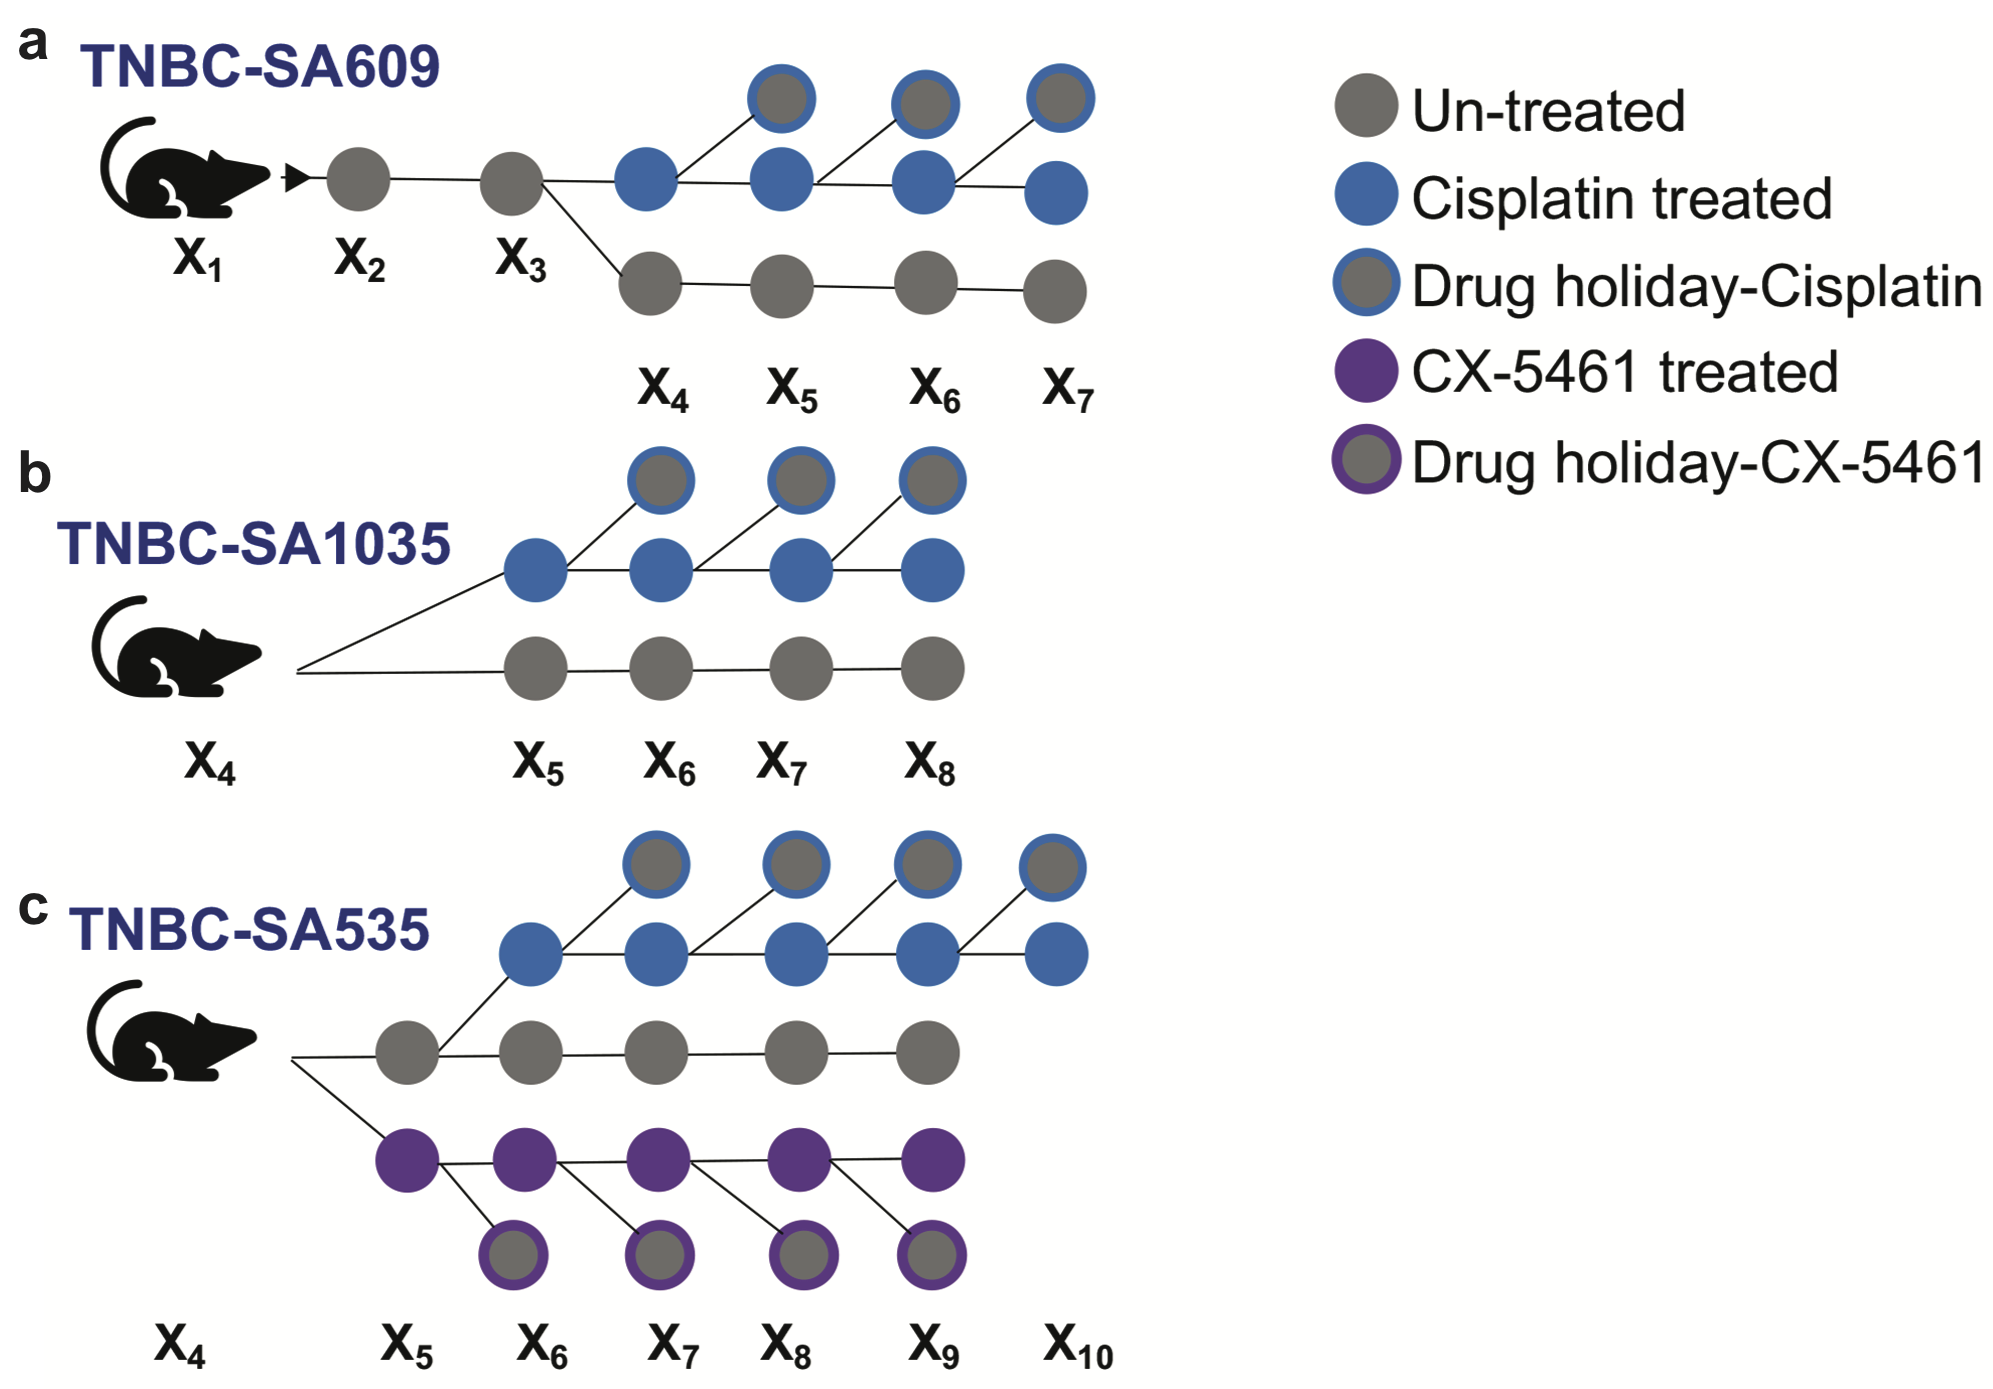
\includegraphics[width=\textwidth]{Figures/chap5/SchematicsforRNAsampling.png}
	
\caption[SchematicsforRNAsampling]
	{\small
	\textbf{Time series sampling and treatment conditions used for scRNA-seq analysis.}
	Each circle indicates patient derived xenograft tumour. All blue circles denote cisplatin treated tumours while purple circles denote CX5461 treated tumours. Grey with blue outline are ciplatin drug holiday samples while grey with purple outline present CX5461 drug holiday tumours. X with subscript numbers indicates the respective passage number of that time series. 
	   \textbf{(a)} TNBC-SA609.
	    \textbf{(b)} TNBC-SA1035.
	    \textbf{(c)} TNBC-SA535.
	}
	\label{fig:RNAsampletree}
\end{figure}
 
 
\subsubsection{Summarization of number of cells and overall read counts of the data}
Tumours from each time point of TNBC-SA609, TNBC-SA1035 and TNBC-SA535 (cisplatin, CX5461) were collected and enzymatically digested with collagenase/hyaluronidase at 37\textdegree C \textbf{(see methods)}, for single cell RNA sequencing (scRNA-seq) as DLP+ (\textbf{\autoref{fig:RNAsampletree}}). In Chapter 3, it was described that tumour dissociation with collagenase enzyme at warmer temperature produces stress response that is minimized
by dissociation at cold temperature. For the experiments of this chapter, I chose to use collagenase enzyme because the tumour dissociation for the DLP+ libraries in Chapter 4, were also performed using the same enzyme. In addition, the chemotherapies are known to produce stress responses and I did not want to mask the expected biological responses by known technical effects. 
%need to fill in the proper number and table from Mirela
From the scRNA-seq libraries, the cells obtained per line ranged from 9220 to 33881 after filtering for high quality cells, representing 212 to 4869 cells per time point sample (median: 800 cells) (\textbf{\autoref{tab:nofcellsRNA}}). 

%---------------------------------------------------------------

\begin{figure}
\centering
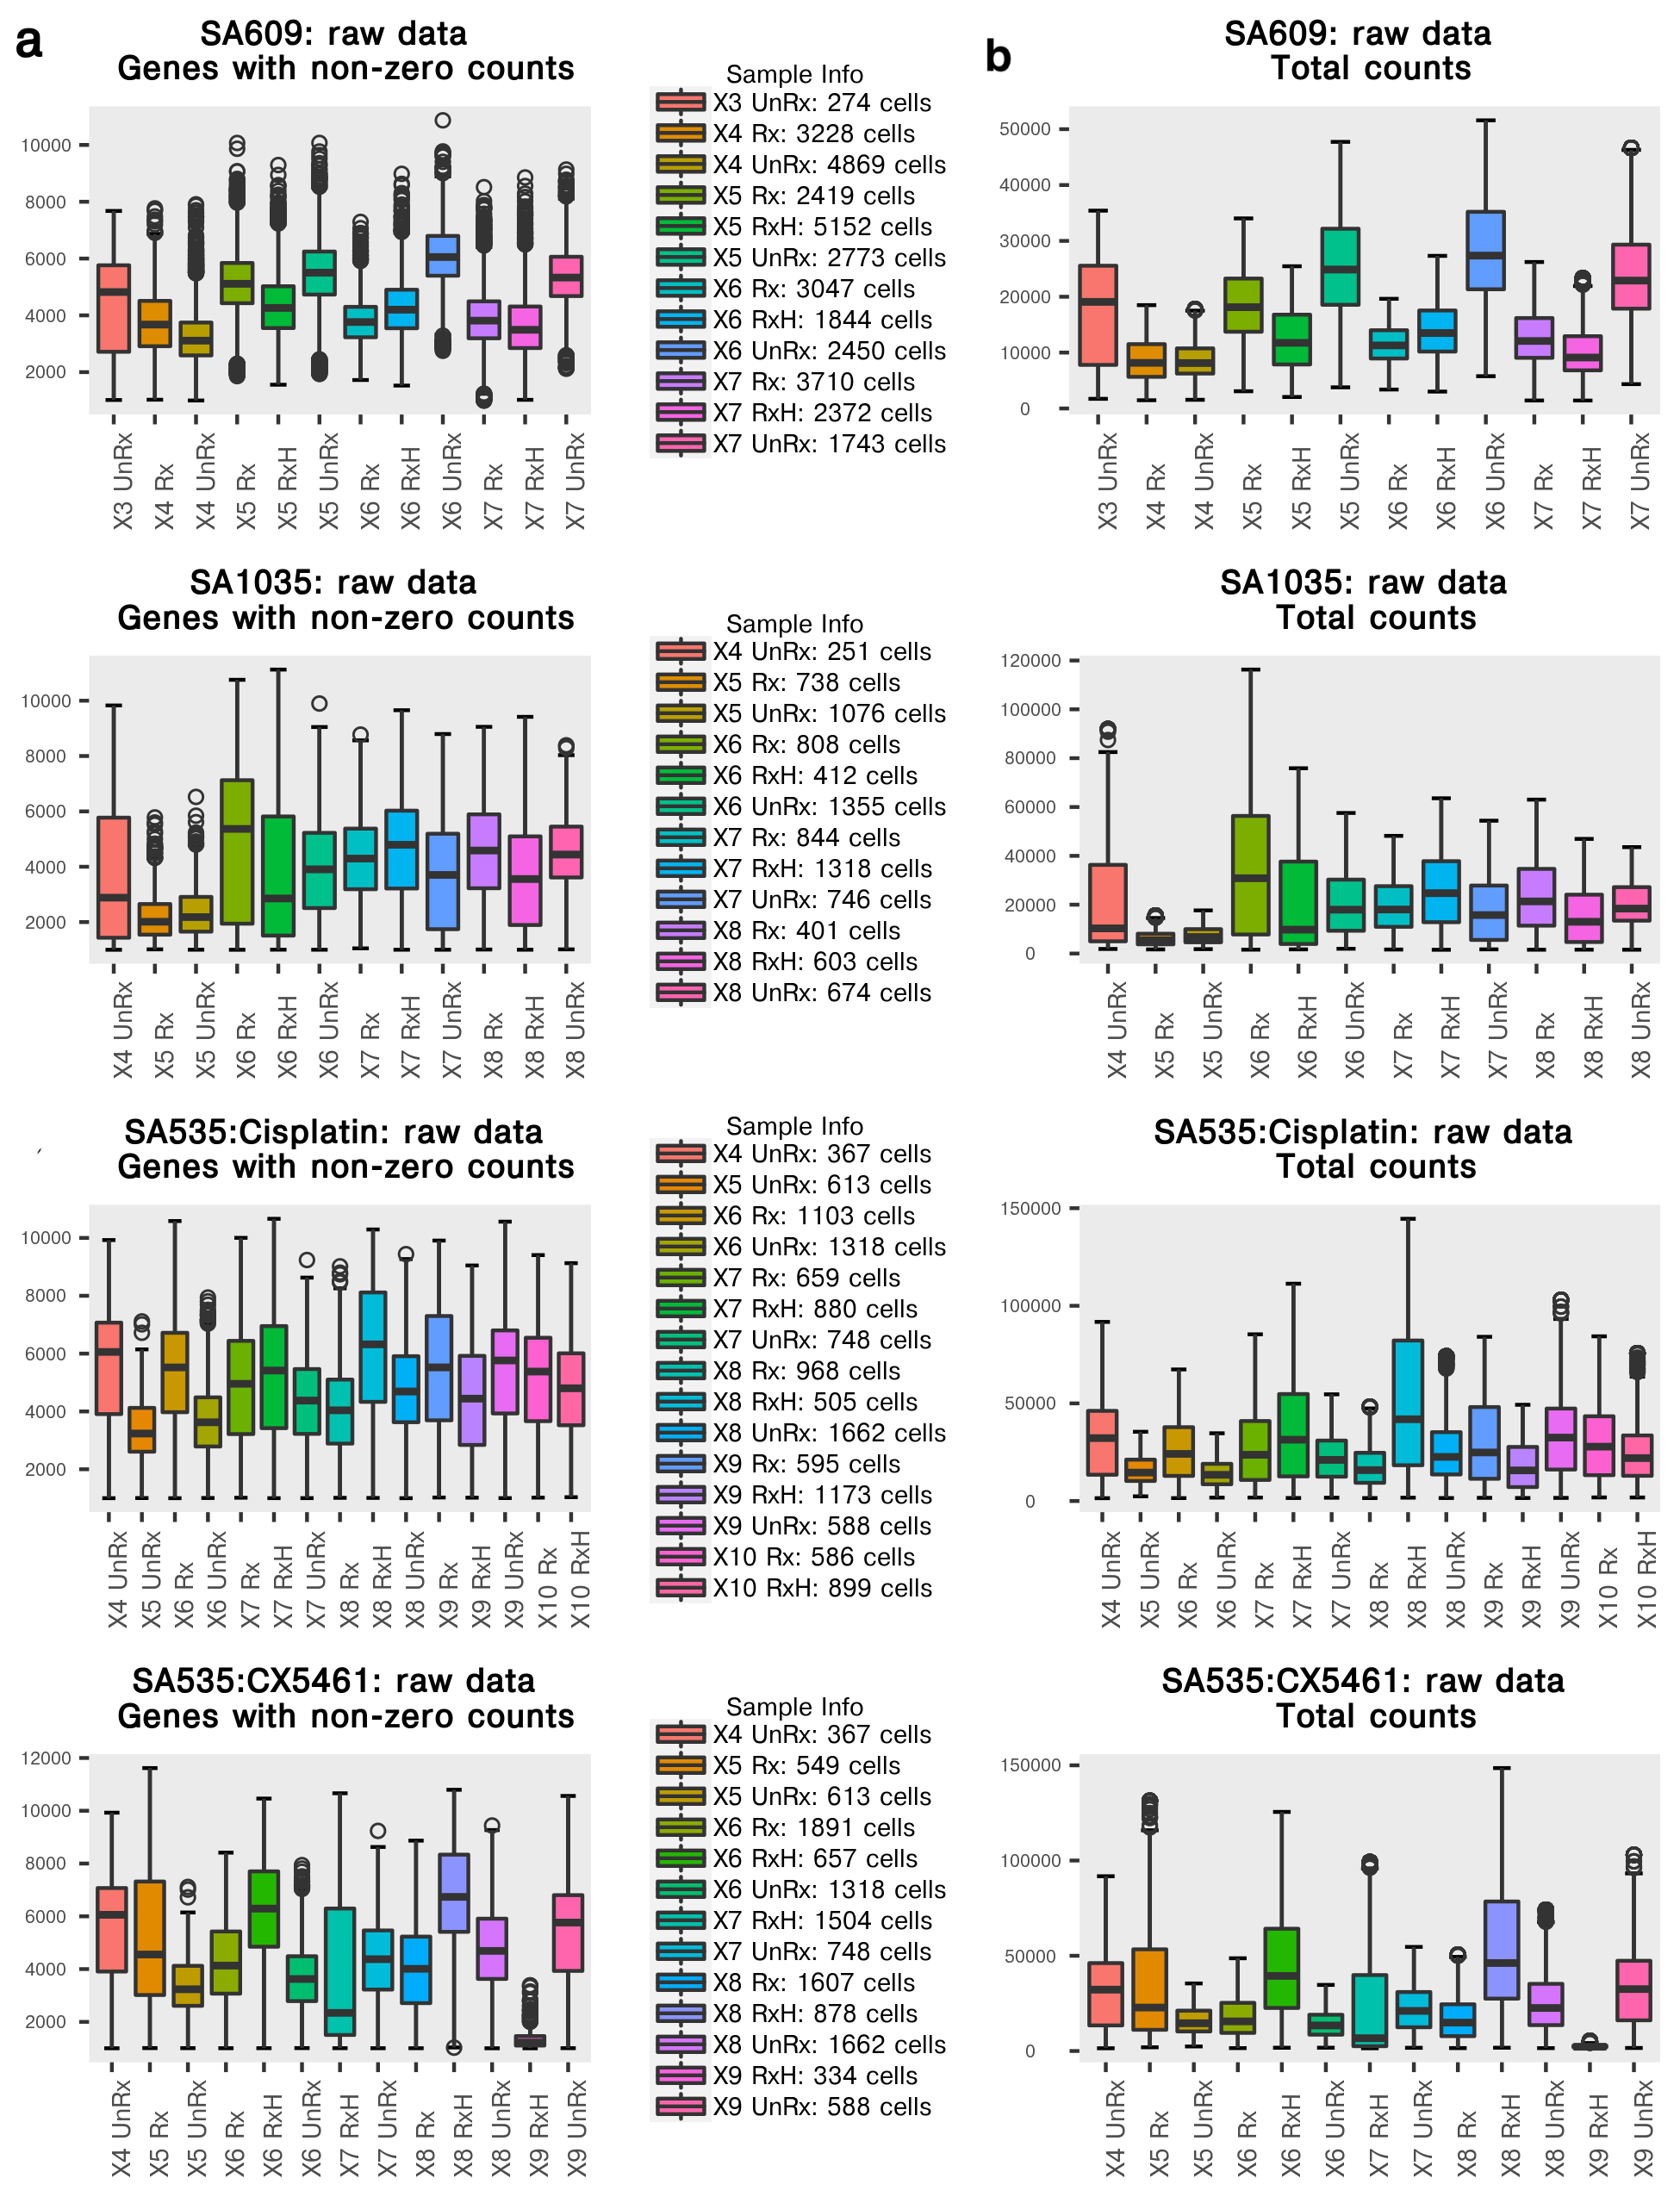
\includegraphics[width=\textwidth]{Figures/chap5/Diagnosticplotsreadcounts.png}
	
\caption[Summary of overall read counts and features of the raw data presented.]
	{\small
	\textbf{Summary of overall read count of the data presented.}
	   All horizontal axes: different batches of experiments and vertical: genes with non zero counts and lines in the boxes are the medians.
	   \textbf{(a)} Number of ``genes with non-zero counts'' for all batches of experiments. 
	    \textbf{(b)} Cell level metric ``total cell counts'' for all batches of experiments.
	   
	}
	\label{fig:Diagnosticplotsreadcounts}
\end{figure}


Moreover, in all 4 TNBC PDX timeseries, the features by count (number of genes with non-zero counts value) ranged from 3826 to 4878 (interquartile range of 3109 to 6320) and total counts per cell medians ranged from 14043.6 to 27805.5 in over all samples (interquartile range of 4342.2 to 63899) \textbf{\autoref{fig:Diagnosticplotsreadcounts}}. 

%\begin{itemize}
   % \item Series SA609: total counts - median over all samples: 14043.6 interquartile range: [4508-17752.2]   number of genes with non-zero counts - median over all samples: 4283.9 interquartile range: [3109-6053]
%\item Series SA1035: total counts - median over all samples: 21935.2 interquartile range: [4342.2-48549.8]   number of genes with non-zero counts - median over all samples: 3826 interquartile range: [2013-5366] 
%\item Series SA535:Cisplatin: total counts - median over all samples: 27805.5 interquartile range: [10453.8-63899]   number of genes with non-zero counts - median over all samples: 4878.7 interquartile range: [3236-6320]
%\item Series SA535:CX5461: total counts - median over all samples: 26869 interquartile range: [17787.2-35371]   number of genes with non-zero counts - median over all samples: 4286.2 interquartile range: [3603.5-6057]

%\end{itemize}

The large variability between samples was partly due to batch processing effects in sequencing depth per cell, sample preparation at different timepoints and number of cells obtained, pointing to the need for batch correction and normalization.


%Only 2 libraries in TNBC-SA1035 (X5-UT-CHIP0071 and X5-UU-CHIP0076) had a low quality cells than other libraries (~2500 total features by counts) but acceptable and good enough to use. Other exceptions were TNBC-SA535-CX-5461 treated at time points X7 and X9 with low quality, that was excluded from the downstream analysis. 


%-----------------------------------------------------------

\begin{figure}
\centering
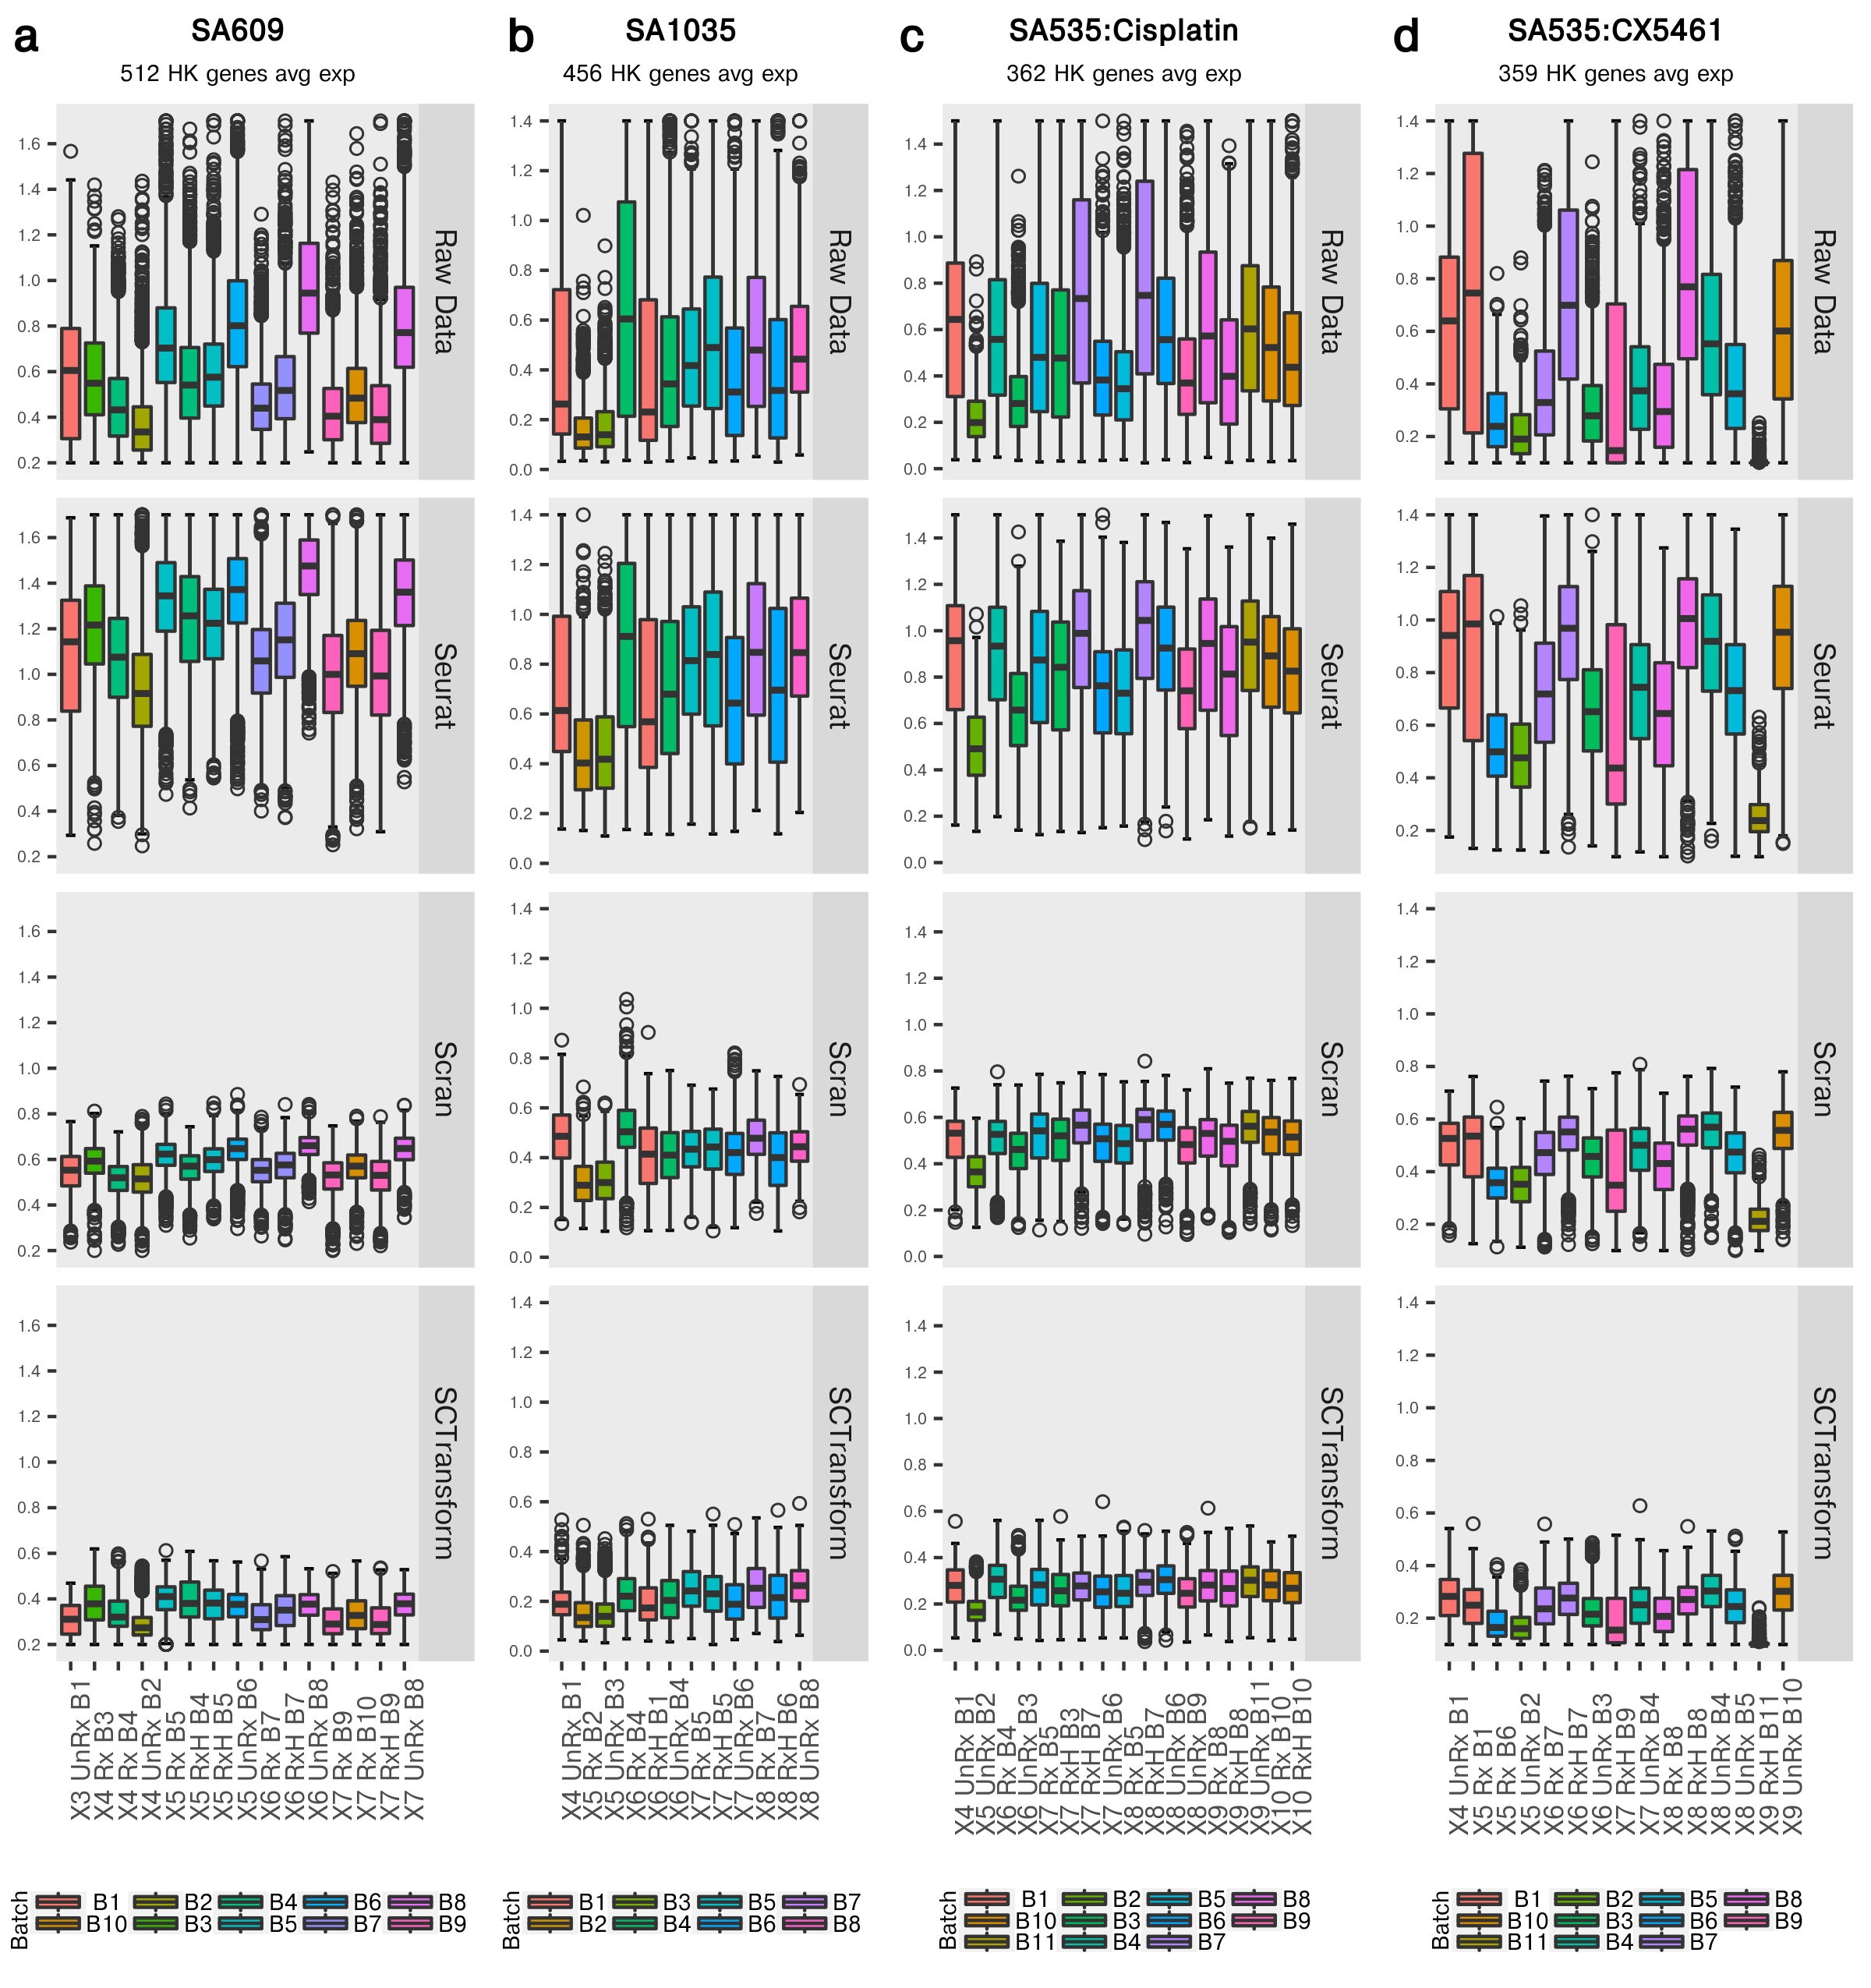
\includegraphics[width=\textwidth]{Figures/chap5/Comparisonofbatcheffects.png}
	
\caption[Summary of overall read count of the data presented.]
	{\small
	\textbf{Evaluation of batch effects in TNBC PDX timeseries data.}
	  House keeping genes were selected from \cite{lin2019evaluating} and mean expression calculated in all timeseries of TNBC PDX. Horizontal axis shows sample IDs from each of that time series and vertical axis shows mean gene expression.
	   \textbf{(a)} Raw data with no normalization showing mean expression of house keeping genes in all 4 treated and untreated TNBC PDX timeseries. 
	    \textbf{(b)} Two times applying \texttt{scran} on data (twice \texttt{scran}) normalization  in all 4 treated untreated TNBC PDX timeseries.
	    \textbf{(c)} \texttt{Seurat} (normalization) on  all 4 treated and untreated TNBC PDX timeseries.
	    \textbf{(d)} \texttt{SCTransform} (normalization) on  all 4 treated and  untreated TNBC PDX timeseries.
	}
	\label{fig:Comparisonofbatcheffects}
\end{figure}



\subsubsection{\texttt{SCTransform} normalization and batch correction of timeseries scRNA-seq data}
%{SCTransform performs more optimal normalization for Single cell RNAseq data in longitudinal \textit{in vivo} experiments}
 %To discern the nature of single cell RNA sequencing data in longitudinal samples, I applied few comparative and diagnostic statistical tools to check the normalization and its effects in my datasets.
The tumour samples for scRNA-seq were collected at different time points because of the nature of experimental design and it was also noted above that large sample variation occurs, suggesting the need for gene expression level sample normalization. 

I considered that a normalization method had good performance if:
\\
\textbf{(1)} it displayed a stable level of normalized house keeping gene expression with low variance across libraries.
\\
\textbf{(2)} it removed the batch effects of gene expression differences. 

 %Errors in normalization can have a significant impact on downstream analysis, such as high false positives in differential expression analysis.
Firstly, I analyzed the variance between samples of 362 to 512 house keeping genes (HK) that expressed in all 4 timeseries dataset. HK genes were identified from the literature as suitable index genes for batch corrections \cite{lin2019evaluating}, selection criteria for HK genes are elaborated in methods.
Since HK genes can also be influenced by treatments,
I conducted analysis with low variance HK genes and found similar results.
Cancer cells are more active than normal cells therefore, HK genes are not completely stable. In the raw data counts, high variance (Interquantile ratio: 0 to 0.86, median: 0.13 to 0.94) across HK genes was found \textbf{(\autoref{fig:Comparisonofbatcheffects} first row}).

Next, I compared the raw data with \texttt{Seurat} \cite{butler2018integrating}, \texttt{scran} \cite{lun2016pooling} and \texttt{SCTransform} \cite{hafemeister2019normalization} normalization methods. 
Notably, both \texttt{SCTransform} (median range: 0.1-0.41 in all timeseries PDX) and \texttt{scran} (median range of 0.21 -0.66 in all in all timeseries PDX) demonstrated low variance between batches, while sample size effect was observed in \texttt{Seurat} output.

However, normalization with \texttt{SCTransform} was able to partially remove batch effects with small range of mean gene expression differences, as shown in  \textbf{\autoref{fig:Comparisonofbatcheffects} a-d, last row}.
Therefore, I selected \texttt{SCTransform} normalization as the best normalization method for downstream analyses in timeseries PDX data. 
 
%Based on series of TNBC-SA1035, SCTransform seems work better than Scran, so  
%Scran: median range: [0.29-0.5]   interquartile: [0.12-0.22]    SCTransform: median range: [0.13-0.26]   interquartile: [0.09-0.17] 
 
 
%-----------------------------------------------------------------

\begin{figure}
\centering
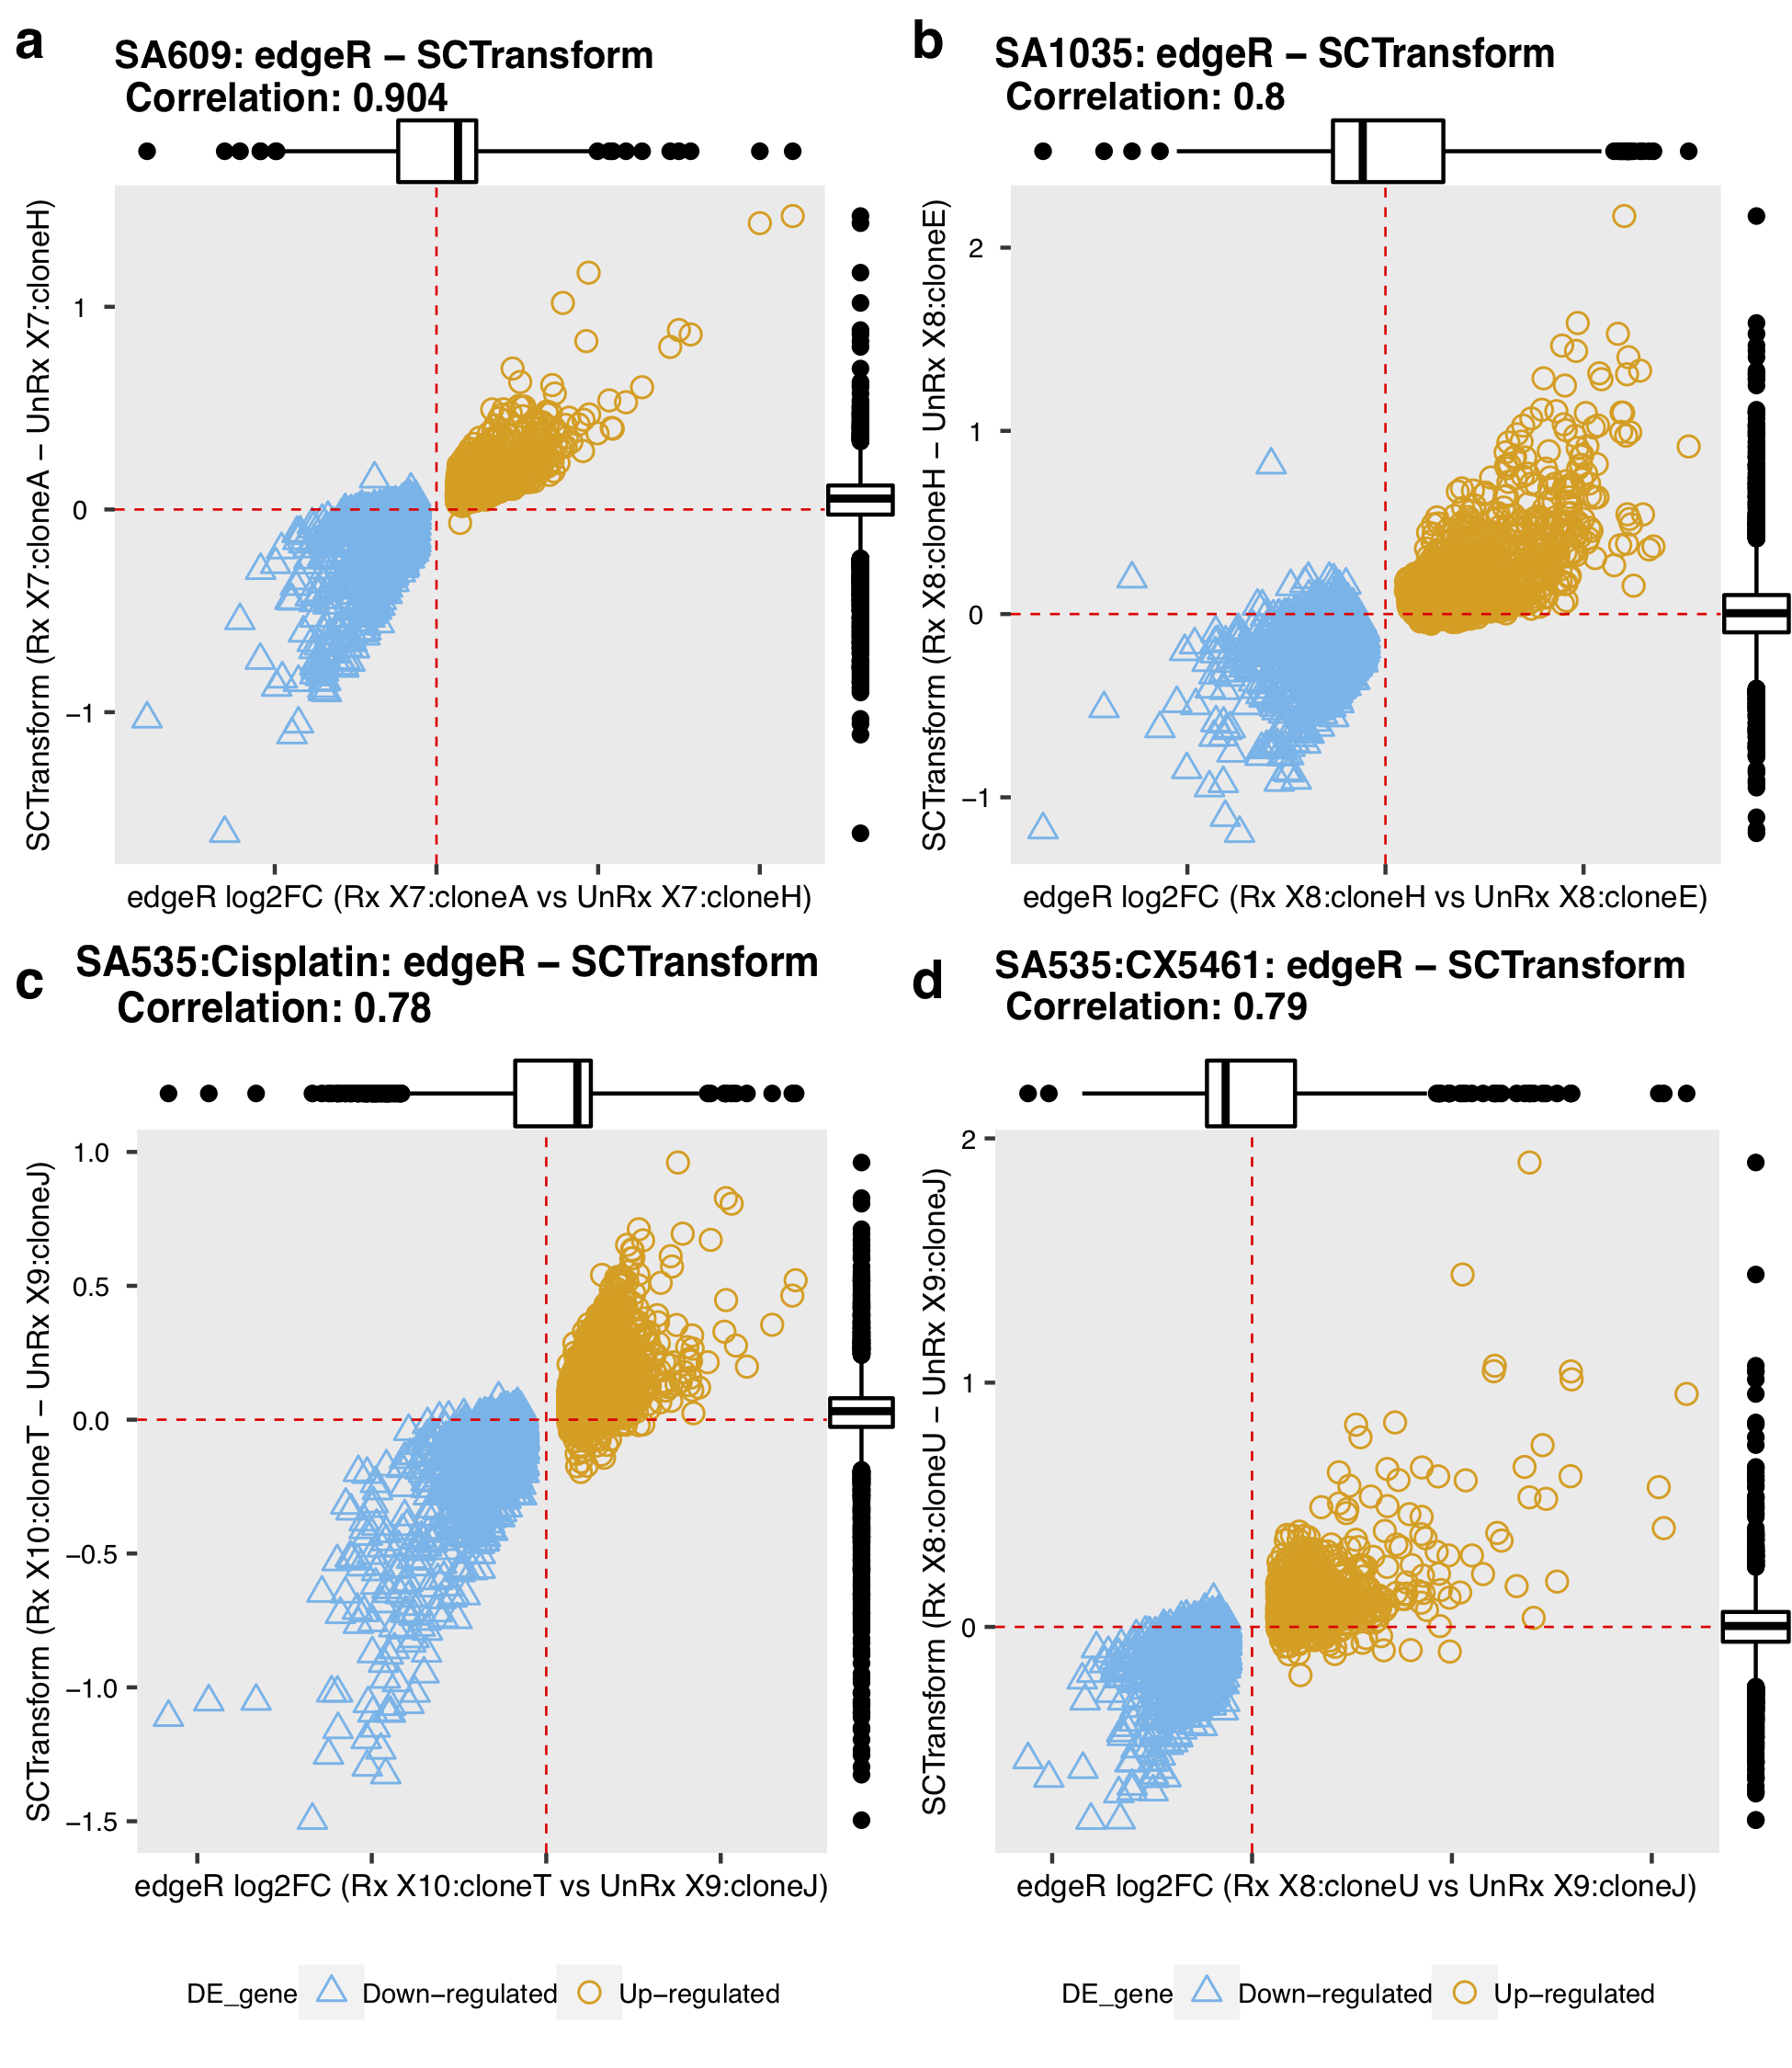
\includegraphics[width=\textwidth]{Figures/chap5/edgeRSCTransformcorrelation.png}
	
\caption[Evaluation of \texttt{edgeR} in all PDX timeseries data.]
	{\small
	\textbf{Comparison of \texttt{edgeR} with \texttt{SCTransform} normalization for downstream data analysis.}
All vertical axes present \texttt{SCTransform} normalized log2 counts gene expression in resistant clone versus log2 counts gene expression in sensitive clone. All horizontal axes present log2 fold change of gene expression for \texttt{edgeR}.	Spearman correlation coefficients and p-values are shown in each panel. Boxplot (top) X-axis shows the distribution of \texttt{edgeR} results, boxplots (right) Y-axis shows the distribution of \texttt{SCTransform} normalized expression results.
	}
	\label{fig:edgeRsctransformcorrelation}
\end{figure}

%---------------------------------------------------------------------

\subsubsection{Detecting differentially expressed genes with \texttt{edgeR}}

Next, I selected \texttt{edgeR} as it is well suited to datasets where batch effects may be a concern because it incorporates information sharing across all genes to improve accuracy of gene-wise dispersion estimation (or differentially expressed genes detection).
\\
A benchmark study evaluated eleven methods for differential expression analysis of RNA-seq transcriptomic data, and showed that \texttt{edgeR} outperformed other methods in differential expression estimation with high accuracy of differentially expressed genes detection, while showing low false discovery rates compared to other methods \cite{soneson2013comparison}. 

However, \texttt{edgeR} performs internal normalization, accepting raw data values as input (quantify the relative changes in expression level between groups of cells rather than provide a normalized expression data), therefore, I sought to evaluate whether differentially expressed (DE) genes that are detected by \texttt{edgeR} are correlated with \texttt{SCTransform} normalization. 

%Spearman ranked correlation function was applied and found that correlation coefficients range from 0.78 to 0.904 with the highest correlation in TNBC-SA609 dataset: 0.904.

I observed that \texttt{edgeR} and \texttt{SCTransform} normalization were strongly correlated in all timeseries datasets. The Spearman correlation coefficients $r$ ranged from 0.78 to 0.9 with the highest correlation in TNBC-SA609 dataset  (\textbf{\autoref{fig:edgeRsctransformcorrelation} a}), followed by TNBC-SA1035 ($r=0.8$),  TNBC-SA535:CX5461 ($r=0.79$),   \textbf{(\autoref{fig:edgeRsctransformcorrelation} b, d}) and the minimum correlation coefficient was 0.78 for TNBC-SA535:Cisplatin ( \textbf{\autoref{fig:edgeRsctransformcorrelation} c}).
\\
Therefore, \texttt{edgeR} was used to establish pairwise sample comparisons and \texttt{SCTransform} was used for comparison across samples.

%-----------------------------------------------------------------


%\subsection{Clone-specific genotypes underpin clone-specific gene expression programs}
% where to put this paragraph?
%Next, I profiled the impact of clone specific gene expression changes as a higher order representation of phenotypic properties. I tested if the genotypes of high fitness clones exhibited changes in their transcriptional program, with scRNA-seq performed on matched aliquots of same samples sequenced using DLP+ on the serially passaged TNBC PDX as mentioned previously (\textbf{\autoref{fig:RNAsampletree}}.



\begin{figure}
\centering
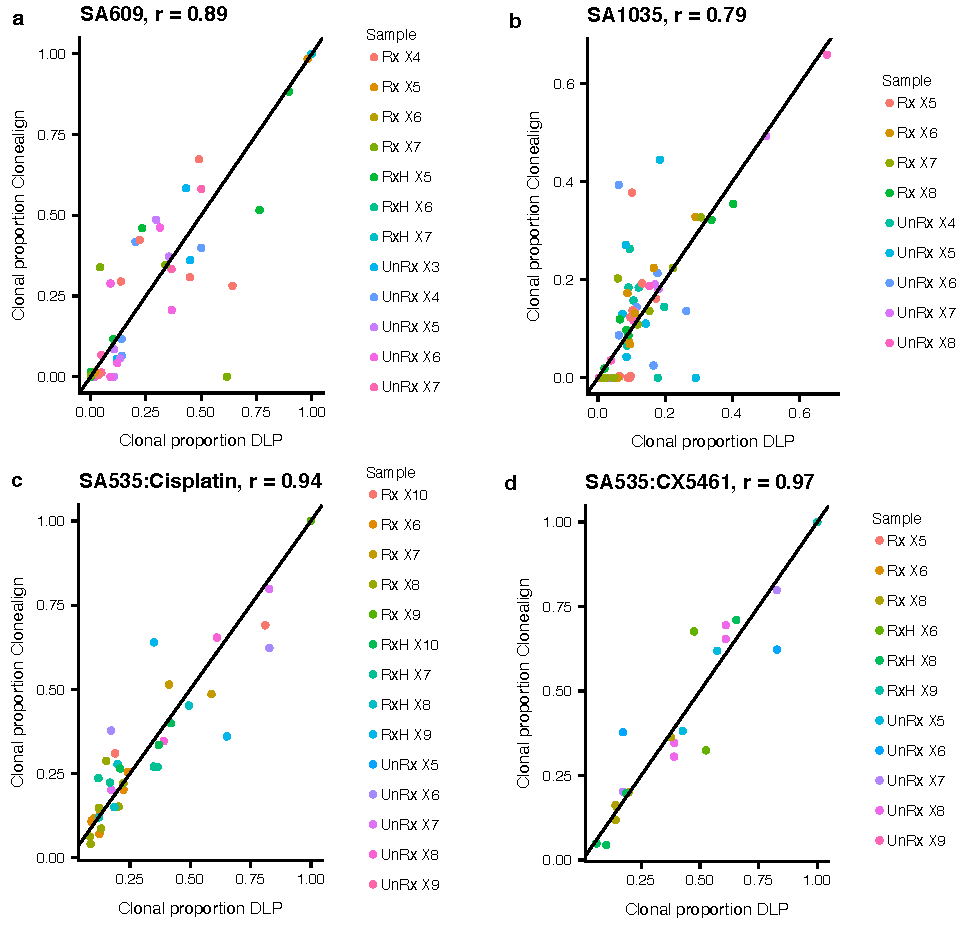
\includegraphics[width=\textwidth]{Figures/chap5/fig6_clonealign_correlation.pdf}
	
\caption[\texttt{clonealign} clonal proportions vs. DLP+ clonal proportions]
	{\small
	\textbf{\texttt{clonealign} clonal proportions vs. DLP+ clonal proportions.} Horizontal axis represents DLP clonal proportions while vertical axis represents clonealign defined clonal proportion. Rx: Treated; UnRx: Untreated; RxH: drug holiday.
	 \textbf{(a)} TNBC-SA609.
	   %indicating positive correlation (Pearson correlation from $r \geq 0.89$).
	 \textbf{(b)} TNBC-SA1035.
	 %and Pearson correlation is $r \geq 0.78$.
	 \textbf{(c)} TNBC-SA535:Cisplatin.
	 %and Pearson correlation is $r \geq 0.94$ for cisplatin treated.
	 \textbf{(d)} TNBC-SA535:CX5461. Pearson correlation coefficients are shown in each panel.
	}
	 
	\label{fig:Clonealigncorrelation}
\end{figure}



%--------------------------------------------------------------------


\subsubsection{Relative abundance of copy number assigned scRNA-seq clonal subpopulations were strongly correlated}
 
To assign scRNA-seq cells to DLP+ defined clones in each sample (Chapter 4), I applied \texttt{clonealign} \cite{campbell2019clonealign}, a statistical method that made a probabilistic assignment of scRNA-seq cells to a priori copy number determined clones, under the assumption that copy number alterations will also alter transcript levels in autosomal chromosomes. \texttt{clonealign} used raw data after quality control filter, mouse and doublet removal but before normalization.
 
I observed that the relative abundance of \texttt{clonealign} assigned clone memberships for 10x data were well correlated with the previously observed clonal fractions of CNA determined clones \textbf{(\autoref{fig:Clonealigncorrelation}}). TNBC-SA535 treated with CX-5461 (11 libraries) presented the highest Pearson correlation of 0.97 (p-value$< 10^{-15}$), followed by its cisplatin treated branch (14 libraries) with a Pearson correlation of 0.94 (p-value$< 10^{-18}$,  \textbf{\autoref{fig:Clonealigncorrelation} c, d}). TNBC-SA609 PDX timeseries (12 libraries) presented a Pearson correlation coefficient of 0.89 (p-value $< 10^{-16}$, \textbf{\autoref{fig:Clonealigncorrelation} a}), while TNBC-SA1035 (9 libraries) exhibited the lowest value of Pearson correlation of 0.78 (p-value$< 10^{-18}$) among all four series \textbf{(\autoref{fig:Clonealigncorrelation} b)}.
  
  
\subsubsection{Single cell copy number clonal structure observed in UMAP summarized transcriptomes with residual batch effects}

The observed \texttt{clonealign} transcriptome correlations were consistent with a signficant transcriptome signal from CNA differences.  To further illustrate this relationship, I summarized the \texttt{SCTransform} normalized scRNA-seq expression of cells using UMAP dimensionality reduction \cite{becht2019dimensionality}, with the clonal assignments of cells shown as embeddings. 

 I found that scRNA-seq embeddings displayed a dynamic pattern of global expression over time with and without treatment, which tracked with clone assignments indicating co-variation of transcriptional properties with clonal abundance. UMAP visualization of clusters identified that \textbf{clone H} cells clustered together at the last time point along with \textbf{clone C} in untreated setting; \textbf{clone A} cells clustered together in the cisplatin treated series of TNBC-SA609 PDX (\textbf{\autoref{fig:EmbeddingsRNA} a}), purified over time matching their genomically defined counterparts (\textbf{\autoref{fig:EmbeddingsRNA} b}). Similarly, \textbf{clone E} in untreated and \textbf{clone H} in treated timeseries of TNBC-SA1035  (\textbf{\autoref{fig:Clonealigncorrelation} c}) clustered uniquely at the later time points. \textbf{\autoref{fig:EmbeddingsRNA} d} shows the clonal proportions at each time point in DLP+ emerging with and without treatment from Chapter 4 in TNBC-SA1035. 

TNBC-SA535 PDX (untreated, treated with cisplatin and treated with CX5461) exhibited aggregation of similar patterns of cell clusters that favoured the emergence of genomic clones in their respective series (\textbf{\autoref{fig:EmbeddingsRNA} e, f}). \textbf{Clone J} (purple) in untreated control timeseries \textbf{(\autoref{fig:EmbeddingsRNA} e, top panel)}, \textbf{clone T} (red) in cisplatin treated \textbf{(\autoref{fig:EmbeddingsRNA} e, middle panel)} and \textbf{clone U} (dark brown) in CX5461 treated \textbf{(\autoref{fig:EmbeddingsRNA} e, lower panel)} exhibited approximately similar proportions with respect to other clones as observed in DLP+ (\textbf{\autoref{fig:EmbeddingsRNA} f}). 

  
 
\begin{figure}
\centering
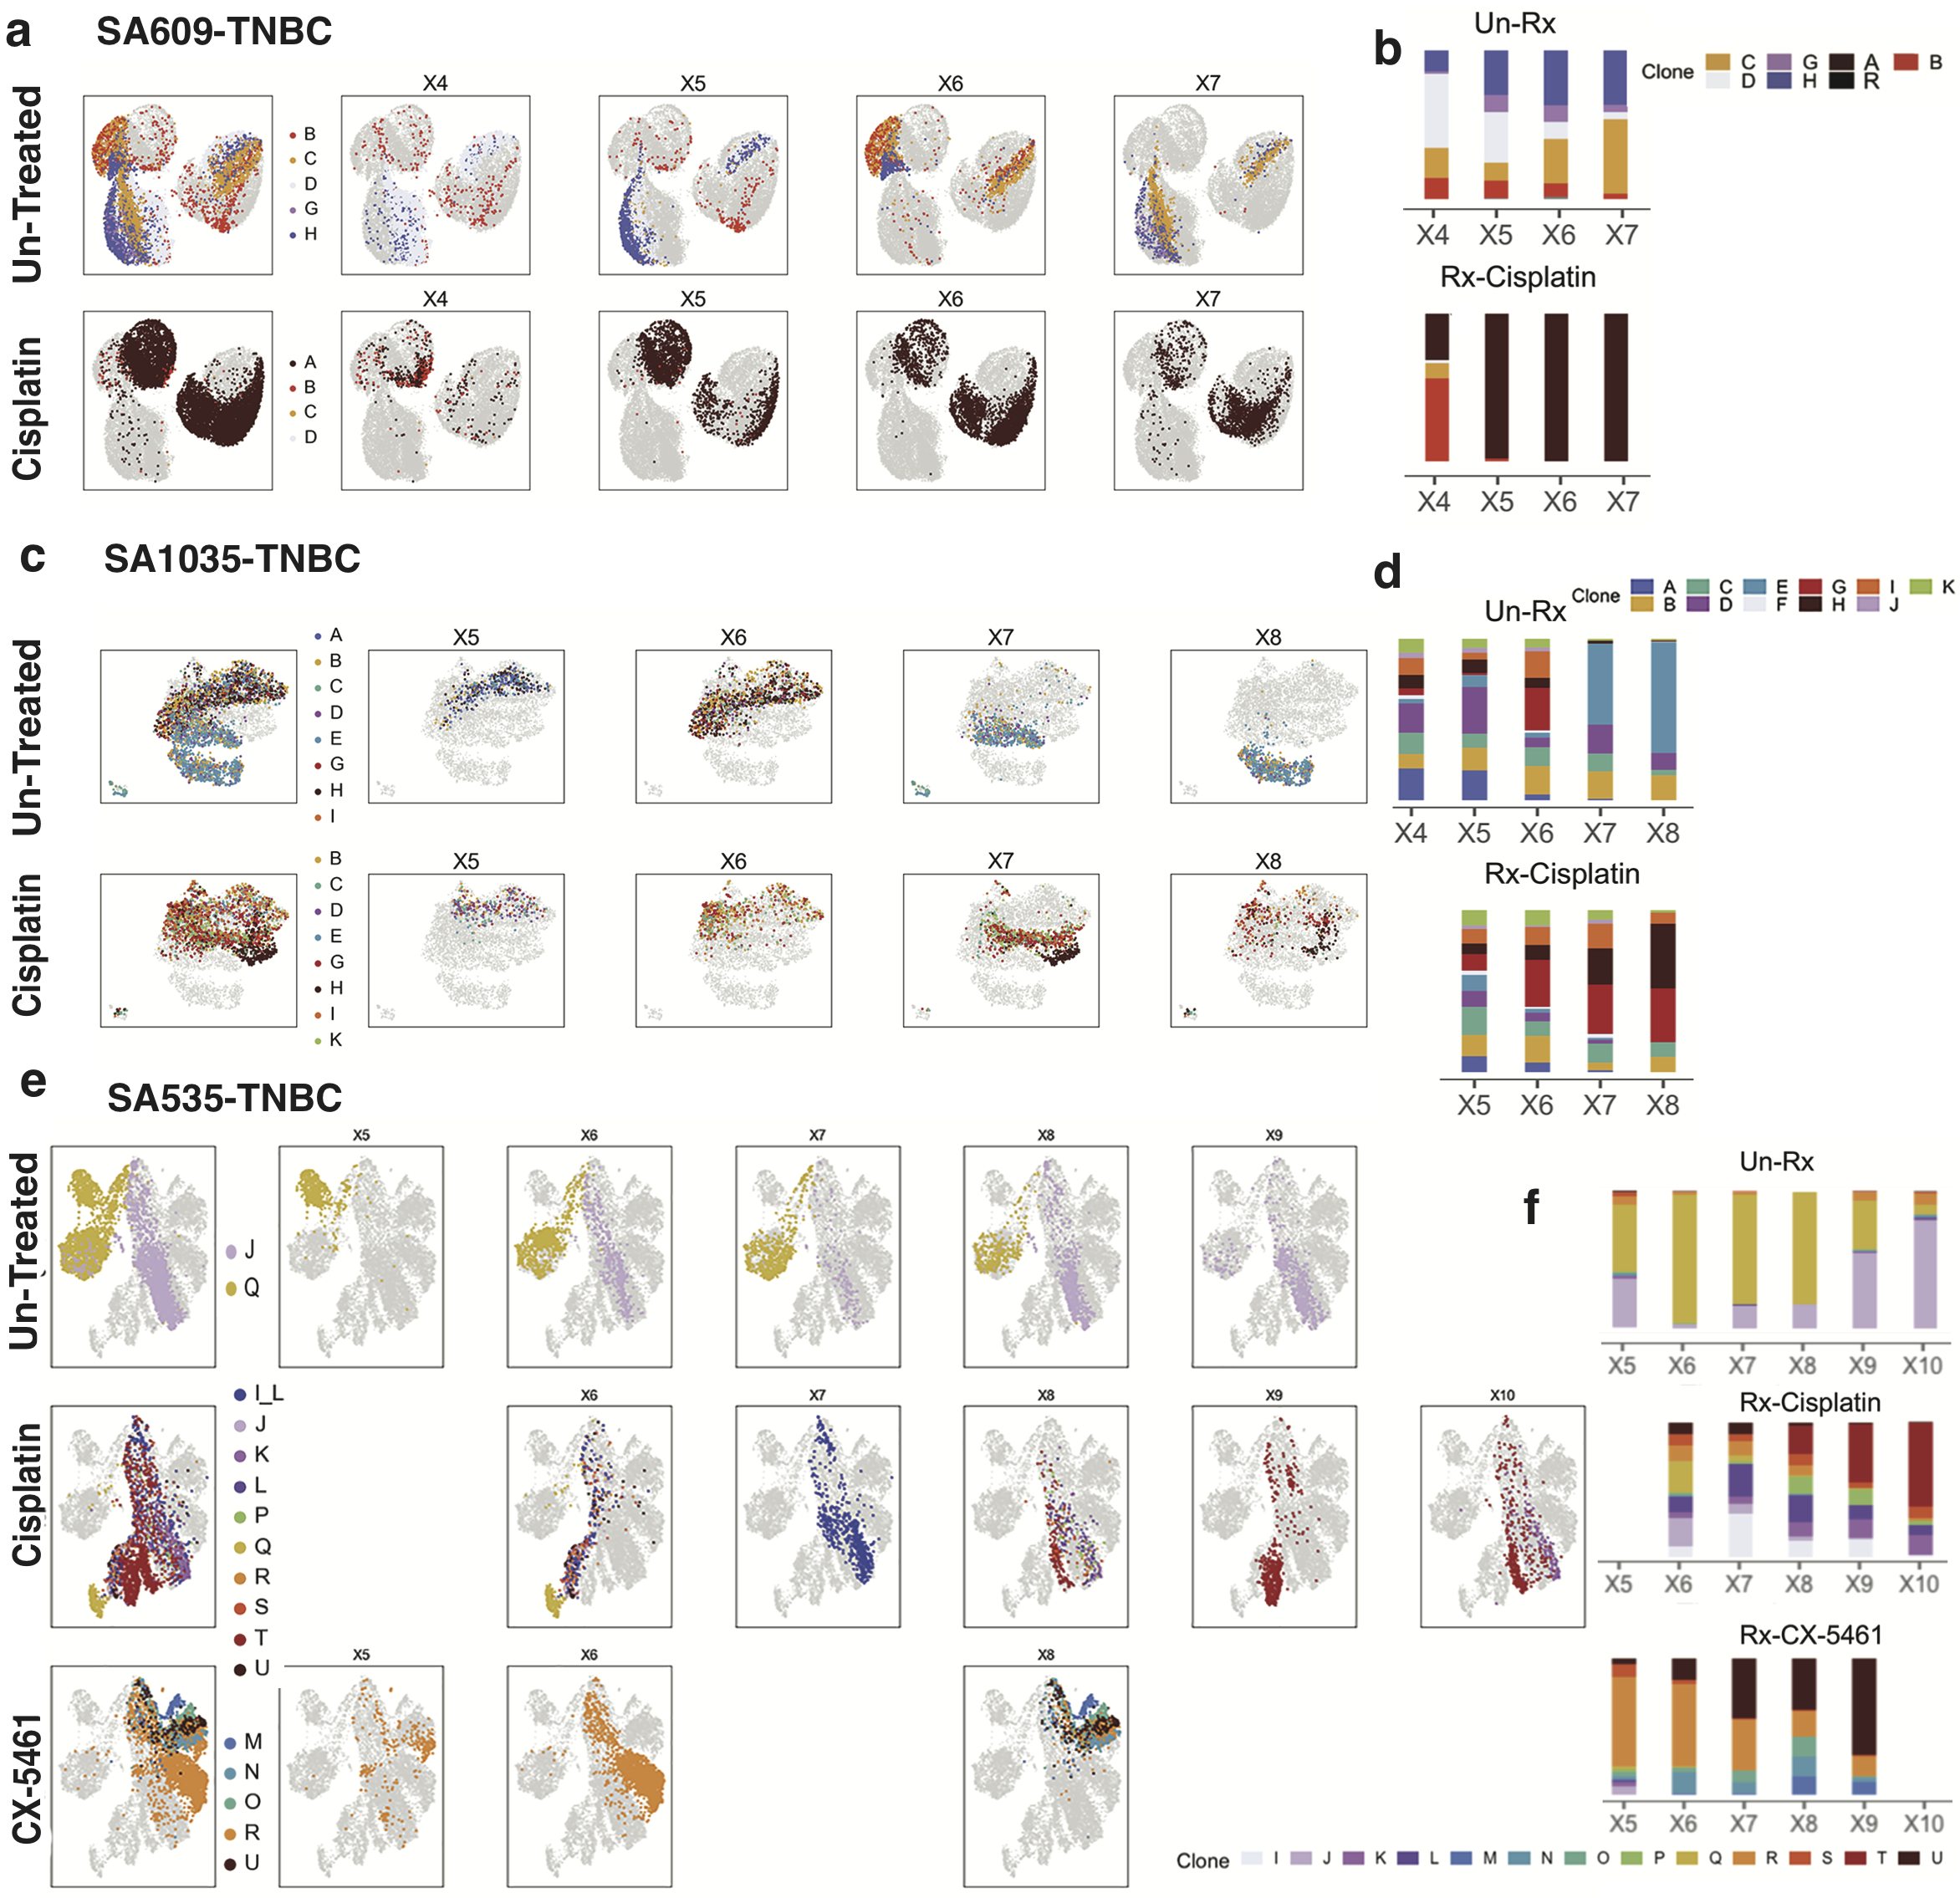
\includegraphics[width=\textwidth]{Figures/chap5/EmbeddingsRNA.png}
	
\caption[Gene expression impacts of clone-specific copy number profiles]
	{\small
	\textbf{Gene expression impacts of clone-specific copy number profiles.}
	\textbf{(a, c, e)} Low dimensional \ac{UMAP} embeddings of  scRNA-seq libraries across the TNBC timeseries, for SA609, SA1035 and SA535, respectively. The leftmost panels show all timepoint embeddings annotated with \texttt{clonealign} assignments. The remaining panels show individual timepoint embeddings.
	\textbf{(b, d, f)} Barplots recalling clonal proportion from DLP+ of SA609, SA1035 and SA535, respectively, taken from Chapter 4 with and without drug. 
	}
	\label{fig:EmbeddingsRNA}
\end{figure}

%---------------------------------------------------------------- 

Despite normalization and batch correction with \texttt{SCTransform}, some residual batch effects can be seen in the UMAP embeddings of TNBC-SA1035, X7 to X8 (\textbf{\autoref{fig:EmbeddingsRNA} c}). The major clone E (blue) along with minor clones, B and D,  clustered in two different dimensions in untreated passages X7 and X8. However, they clustered together indicating that even though there are some residual batch effects remaining, the cells belonged to the same group.

%---------------------------------------------------------------

\subsection{Contrasts of resistant and sensitive clone specific gene expression reveals the contribution of \textit{in cis} and \textit{in trans} components}

Next, I sought to quantify the possible impact of CNA on transcription (\textit{in cis}) in contrast with regions of the genome unaffected by CNA differences between clones.

%Following the above results of copy number mediated effects on transcriptome phenotype, I set out to estimate the proportion of the transcriptome affected \textit{in cis} versus that affected \textit{in trans}. 

I analysed differentially expressed (DE) genes by comparing resistant clones from all the 4 treated timeseries PDX versus sensitive clones of all the timeseries PDX at the same passage. A  differentially expressed (DE) gene is defined as regulated \textbf{\textit{in cis}}, if there was a difference in median copy number for that gene between the two compared clones, and \textbf{\textit{in trans}}, if the median copy number remains the same but the gene is differentially expressed between resistant and sensitive clones (either upregulated or downregulated). Also, \textbf{{\textit{In cis} positive tendency}} means that the gene expression is up or down regulated, with a gain or loss in copy number, respectively, whereas, \textbf{{\textit{in cis} negative tendency}} means that the gene expression is paradoxically changing with change in copy number. However, \textbf{\textit{in trans}} genes are independent of copy number change.

To determine how much of the transcriptome is modulated by \textit{in cis} and \textit{in trans}. I studied clones of high and low fitness in untreated and treated regimes, as determined in Chapter 4.

%I assumed that the clones that showed fitness advantage under drug selection were resistant because they were high abundance clones (tumour growth inhibition was low in those tumours), whereas the clones that had high fitness coefficients in the absence of drug were sensitive because they could not survive under drug pressure but showed fitness advantage over others in the absence of drug. 
 In SA609: \textbf{clone A} (Resistant), \textbf{clone H} (Sensitive);  SA1035: \textbf{clone H} (Resistant), \textbf{clone E} (Sensitive); SA535:Cisplatin: \textbf{clone T} (Resistant), \textbf{clone J} (Sensitive); SA535:CX541: \textbf{clone U} (Resistant), \textbf{clone J} (Sensitive). 
 
 %------------------------------------------------------
% Table generated by Excel2LaTeX from sheet 'Sheet1'
 \begin{table}[bp]
   
   \centering
   \caption{List of resistant and sensitive clones across TNBC PDX.} 
   %The boldface clones are the most resistant and sensitive and.
     \begin{tabular}{|l|l|l|}
      \hline
     TNBC PDX & Resistant clones & Sensitive clones \\
     \hline
     TNBC-SA609  & \textbf{A}, B & \textbf{H}, C \\
     TNBC-SA1035 & \textbf{H}, G & \textbf{E} \\
     TNBC-SA535:Cisplatin & ST, R, \textbf{T} &  \textbf{J}, Q \\
     TNBC-SA535:CX5461 & \textbf{U}, R, MNO &  \textbf{J}, Q \\  
     \hline
     \end{tabular}%
   
   \label{tab:Listofresistantandsensitiveclones}%
 
 \small{Bold clone names identify the most resistant and sensitive clones based on Chapter 4. The others were closely related, therefore included in some of the analysis for comparison}.  
 
 \end{table}%
%--------------------------------------------------------------------
However, for more detailed analysis of proportions of \textit{in cis} and  \textit{in trans} genes, some of the clones that  were closely related to the resistant clones or having second highest fitness coefficients in DLP+ data from Chapter 4 were also added (\textbf{\autoref{tab:Listofresistantandsensitiveclones}}). 

For example, \textbf{clone R} in SA535 was not a resistant clone but it gave rise to two different resistant clones under different drugs. \textbf{Clone Q} stayed in high abundance in earlier untreated passages of SA535. \textbf{Clone S} evolved from \textbf{Clone R} and was in the same clade of resistant \textbf{Clone T}.
I focused on differential expression analysis of the aforementioned clones in order to simplify the analysis.
%------------------------------------------------------------------

\begin{figure}
\centering
  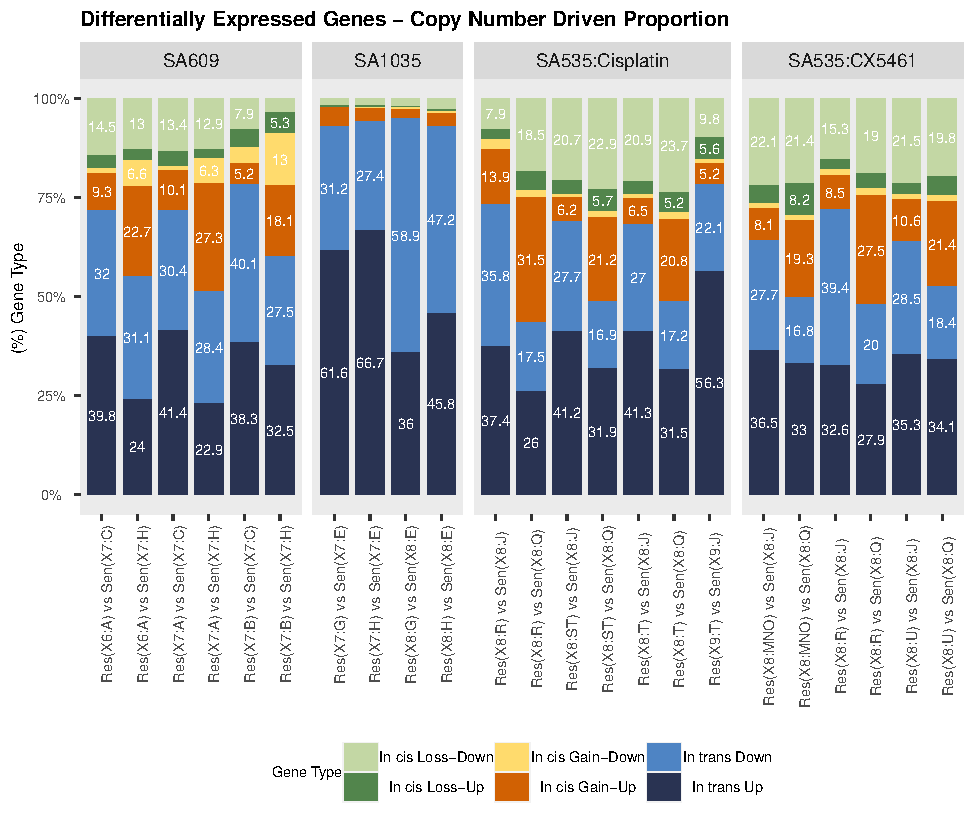
\includegraphics[width=\textwidth]{Figures/chap5/fig4Summaryincistrans.pdf}
	
\caption[Summary proportion of \textit{in cis} and \textit{in trans} regulated gene expression in scRNA-seq data]
	{\small
	\textbf{Proportion of CNA differences mapping to resistant and sensitive clone differentially expressed genes.}
	  Vertical axis represents the percentage of DE genes. Horizontal axis represents the two clones. The numbers written for each coloured bar represent the percentage of the respective category between those two clones, calculated by overlapping positions between chromosome segments and known genes, and assigning those segments to an ensemble gene ID \cite{rainer2019ensembldb} of the  selected \ac{DE} of clones across all timeseries. 
	     
	}
	\label{fig:fig3Summaryincistrans}
\end{figure}

%--------------------------------------------------------------------
\subsubsection{\textit{In cis} expression accounts for {$\sim${~}}5.2\% and {$\sim${~}}56.5\% of clonal differences in resistant vs. sensitive transcriptomes in 4 comparisons}

Using \texttt{edgeR} determined differential expression, I classified genes into \textit{cis} and \textit{trans} up or down regulated, according to the overlap with clone specific copy number differences  (\textbf{\autoref{fig:fig3Summaryincistrans}}).
Notably, it was found that overall, the number of \textit{in trans} genes were higher as compared to \textit{in cis}, which is supporting previously reported results \cite{shao2019copy}. 

Furthermore, I found that \textbf{SA535:Cisplatin} had the highest percentage of \textit{in cis} genes with average of 41.7 (sd=9.67) followed by \textbf{SA535:CX5461} with average of 38.57 (sd=14.0), \textbf{SA609} with average of 35.27 (sd=10.79). The lowest percentage of \textit{in cis} genes were observed in \textbf{SA1035} with average of 6.3 (sd=0.92).

Among differentially expressed genes between resistant and sensitive clones, \textit{in cis} \textbf{upregulated} transcripts associated with CNA gain (in resistant clone) varied from 2.3\% in SA1035 to 31.5\% in SA535:Cisplatin. In contrast, \textit{in cis} \textbf{downregulated} transcripts associated with CNA gain (in resistant clone) varied from 0.1\% in SA1035 to 13\% in SA535:Cisplatin. However, the proportion of \textit{in trans} genes varied from 43.5\% to 94.9\% across all PDX series, \textbf{SA1035} having the highest percentage, with average of 93.7 (sd=0.98).












\subsubsection{Proportions of high essentiality genes, cancer drivers and known cisplatin genes reflect the same proportions of \textit{in cis} and \textit{in trans} in the dataset}
%Next, I asked what proportion of \ac{DE} genes (resistant versus sensitive clones) that intersect with various databases were in \textit{in cis} or \textit{in trans}.
Next, I investigated the proportion of gene functions and pathways associated with \textit{in cis} and \textit{in trans}. To address this, first, I probed four databases, including data DepMap BroadSanger essential gene set \cite{dempster2019agreement}, COSMIC (catalogue of somatic mutations in cancer) \cite{forbes2010cosmic}, ADAM PanCancer Core cancer fitness  \cite{behan2019prioritization}, and cisplatin related genes curated from recent literature (\textbf{\autoref{tab:Cisplatinrelatedgenes}}).

%First, I pulled reference genes from these databases that  intersected with the \ac{DE} dataset and calculated if they are regulated with the change in copy number.
The average proportion of gene set membership over 4 reference gene sets were 10.3\%, 10.44\%, 12.8\% \textit{in cis}, and 16.8\%, 14.02\%, 15\% \textit{in trans} in SA609, SA535:Cisplatin and SA535:CX5461, respectively (\textbf{\autoref{fig:incisgenesindatasets}}).

Consistent with the \textit{in cis/trans} ratio already established that TNBC-SA535 in both treatment regimes inferred the highest of 28\% \textit{in cis} regulated differrentially expressed (DE) genes, whereas TNBC-SA1035 possessed the lowest rate, 2.4\%  of \textit{in cis} DE. On the other hand, TNBC-SA609 showed \textit{in cis} DE gene rate of 12.8\%.

\begin{figure}
\centering
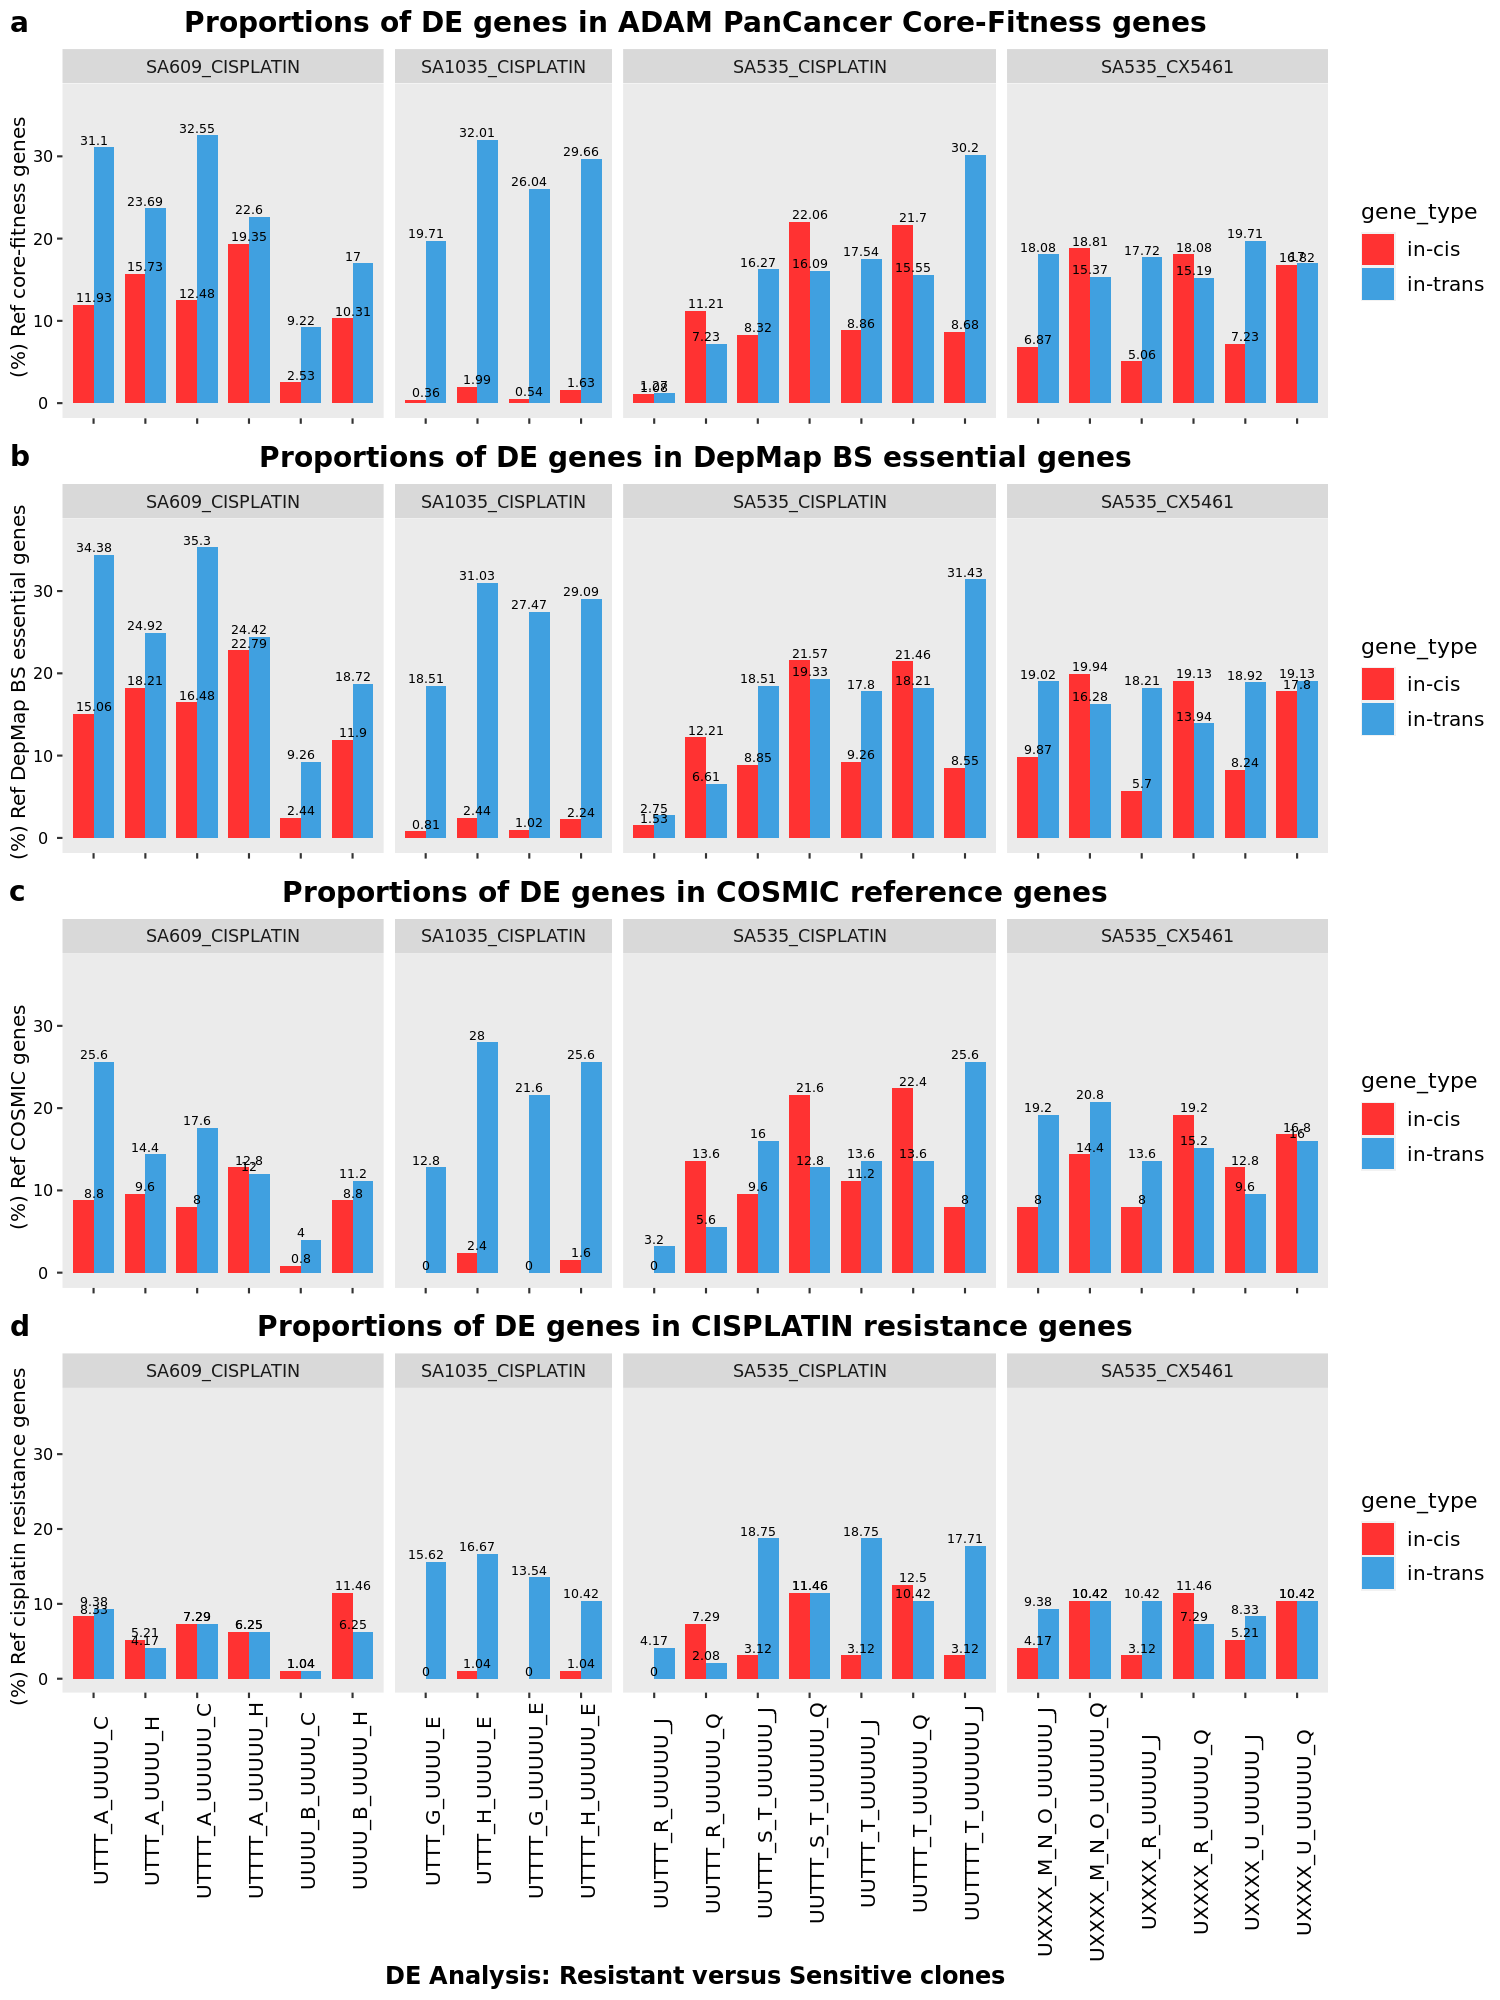
\includegraphics[width=\textwidth]{Figures/chap5/incispercenatgeindatasets.png}

\caption[Summary of number of cisplatin resistance genes \textit{in-cis} and \textit{in-trans}]
	{\small
	\textbf{Mapping \textit{in cis} and \textit{in trans} gene proportions to various datasets.}
	Gene set membership \textit{in cis} and \textit{in trans} differential expression between resistant and sensitive clones. Red bar represent \textit{in cis} proportion, blue represents \textit{in trans}, the star \textbf{(*)} represents significance with p value $<0.05$ (Bootstrapping Confidence Intervals >95\%).
     \textbf{(a)} Proportions of DE genes in ADAM PanCancer Core fitness dataset \cite{behan2019prioritization}. Percentages are written on each bar where red indicates proportion of \textit{in cis} genes and blue indicates the proportion of \textit{in trans} that are matching with the respective list.
     \textbf{(b)} Analogous to  \textbf{a} but the reference dataset is DepMap Broad Sanger essential gene set \cite{dempster2019agreement}.
		\textbf{(c)} Analogous to \textbf{a} but the reference dataset is COSMIC cancer gene set \cite{forbes2010cosmic}.
		\textbf{(d)} Analogous to \textbf{a} but the reference dataset is Cisplatin resistance related gene set (\textbf{\autoref{tab:Cisplatinrelatedgenes}}).

}
    \label{fig:incisgenesindatasets}
    \end{figure}

%------------------------------------------------------------

 Overall, the results remained consistent with the fact that the proportion of \textit{in cis} and \textit{in trans} reflects the degree of CNA alteration in each line, with SA1035 having the lowest proportion of CNA differences between resistant and sensitive clones (1.07\% of DE) and its highest proportion of \textit{in trans} regulated differential expression was 22.4\%.
 
 To show that the above analysis was able to capture significantly expressed genes that demonstrated high impact in cancer genes and matched with cancer core fitness genes from the reference datasets, null hypothesis testing was used. Bootstrap re-sampling of the same number of DE genes, that were found matching in each dataset, was done at random from the genome, to establish confidence intervals more than 95\%. random sampling was done 1000 times and confidence interval was calculated.
\\ 
 The difference was significant in case of large number of reference genes datasets (553 PanCancer, 983 Broad Sanger genes) as highlighted with a star \textbf{(\autoref{fig:incisgenesindatasets} a, b)}, however, null hypothesis could not be rejected in case of insufficient number of reference genes (126 COSMIC, 91 cisplatin resistance genes)\textbf{(\autoref{fig:incisgenesindatasets} c, d)}.





%Then I extract 983 common essential genes that exist in both list to use as our essentiality genes reference, and map our DE genes results with this reference gene set,
%The summary of number of genes and their percentages in each clone comparison in high cancer essentiality gene list (Broad \& Sanger institute) is given in \textbf{\autoref{tab:Broadsanger}}. 

 %In TNBC-SA609 PDX, the mean number of \textit{in cis} genes was 1173.8 (segment positions, $\sigma$ = 494 \textit{in cis} genes, max= 1640, min=215), TNBC-SA1035 presented with the lowest \textit{in cis} with
 %mean value of 187.8 (segment positions, $\sigma$ = 51 \textit{in cis} genes, max=246, min=144). TNBC-SA535 in cisplatin timeseries showed mean number of 1056.9 \textit{in cis} genes (segment positions, $\sigma$ = 624 , max=1900, min=116), whereas, TNBC-SA535 in CX-5461 exhibit highest number of mean \textit{in cis} value of 1400.7 (segment positions, $\sigma$ = 481 \textit{in cis} genes, max=1884, min=739).
 
  
%--------------------------------------------------------------------------------- 


\begin{figure}
\centering
  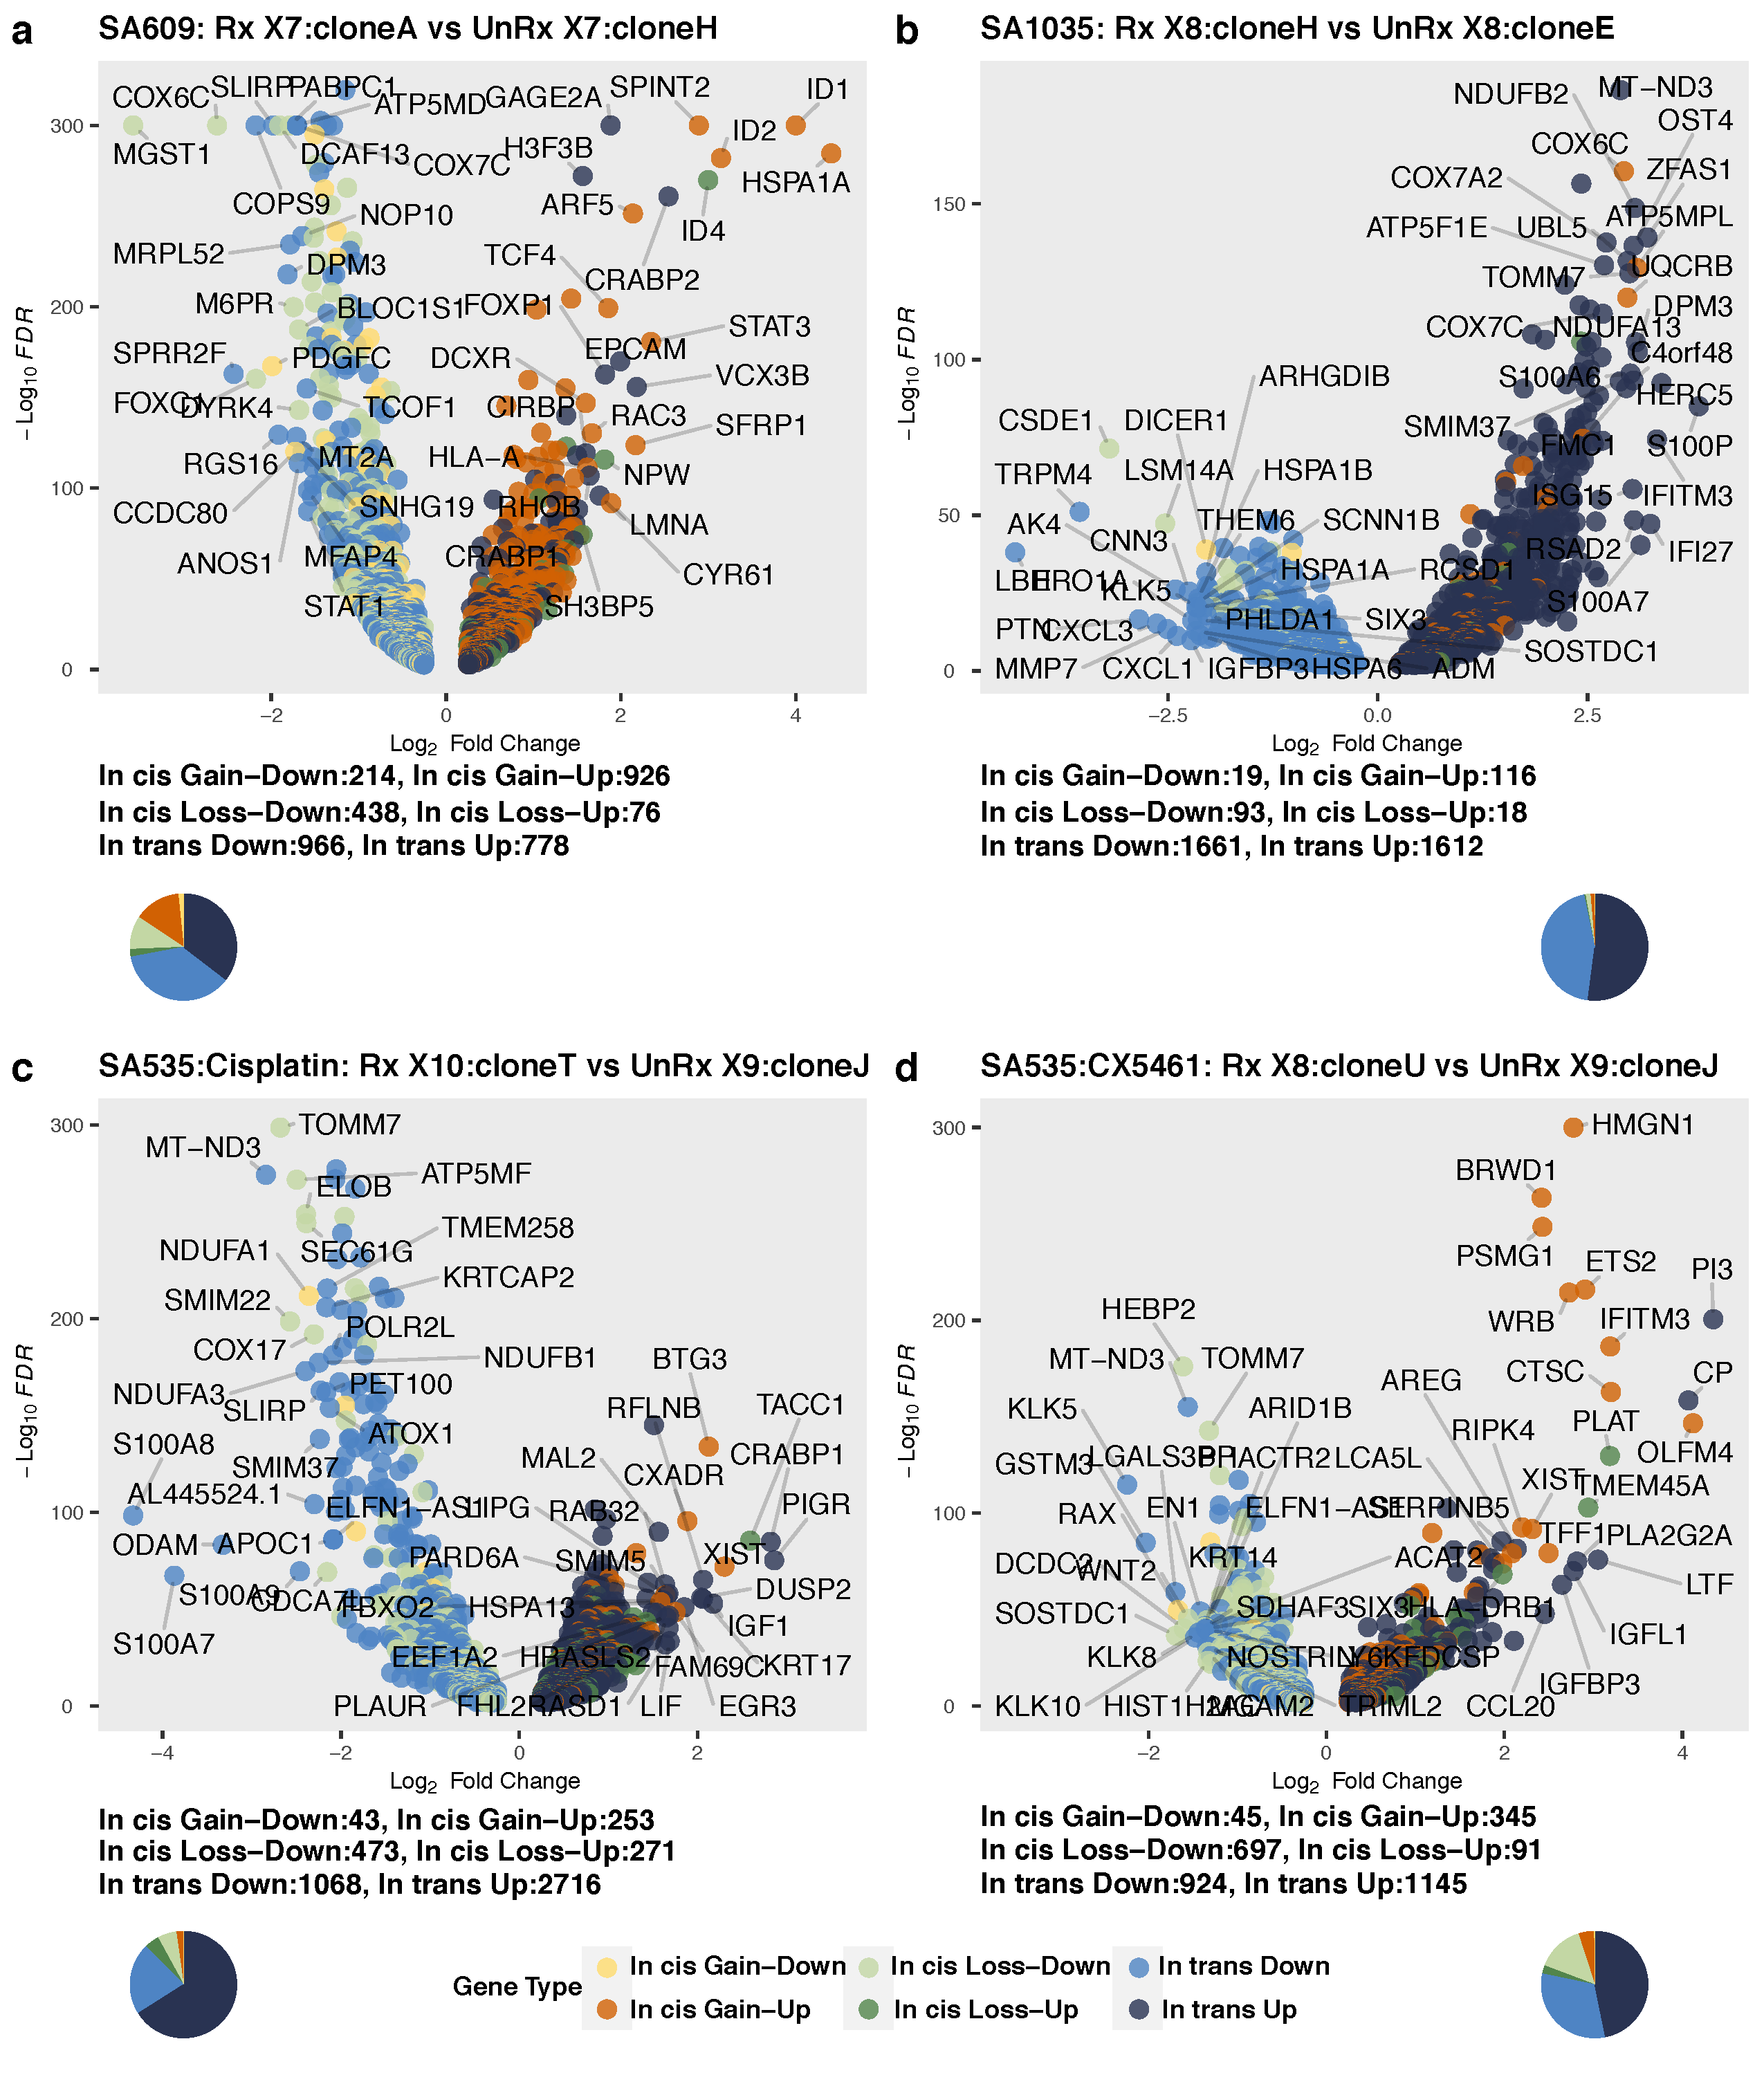
\includegraphics[width=\textwidth]{Figures/chap5/Volcanoes4plots.png}
\caption[DE of resistant and sensitive \texttt{clonealign} defined clones]
	{\small
	\textbf{Differential expression of resistant versus sensitive clones.}
	Horizontal axis shows the logbase 2 fold change values of \texttt{edgeR} differential expression analysis between resistant versus sensitive clones. Vertical axis shows the -log base 10 of false discovery rate (-log10FDR) of ac{DE} genes, colors denote different gene types. 4 pie charts:  proportion of each gene type as in key.
	\textbf{(a)} Volcano plot from SA609 -log10 (FDR) plotted against log2 fold change of pairwise differential gene expression between resistant and sensitive clones. (The threshold for significant genes are FDR p$<$00.01, P Value p$<$00.05, logFC p$>$00.25). \textbf{(b)} Analogous to \textbf{a} but in SA1035. \textbf{(a)} Analogous to \textbf{a} but in SA535:Cisplatin. \textbf{(d)} Analogous to \textbf{a} but in SA535 (CX5461).
	   }
	\label{fig:Volcanoes4plots}
 \end{figure}

%------------------------------------------------------------

\begin{figure}
\centering
  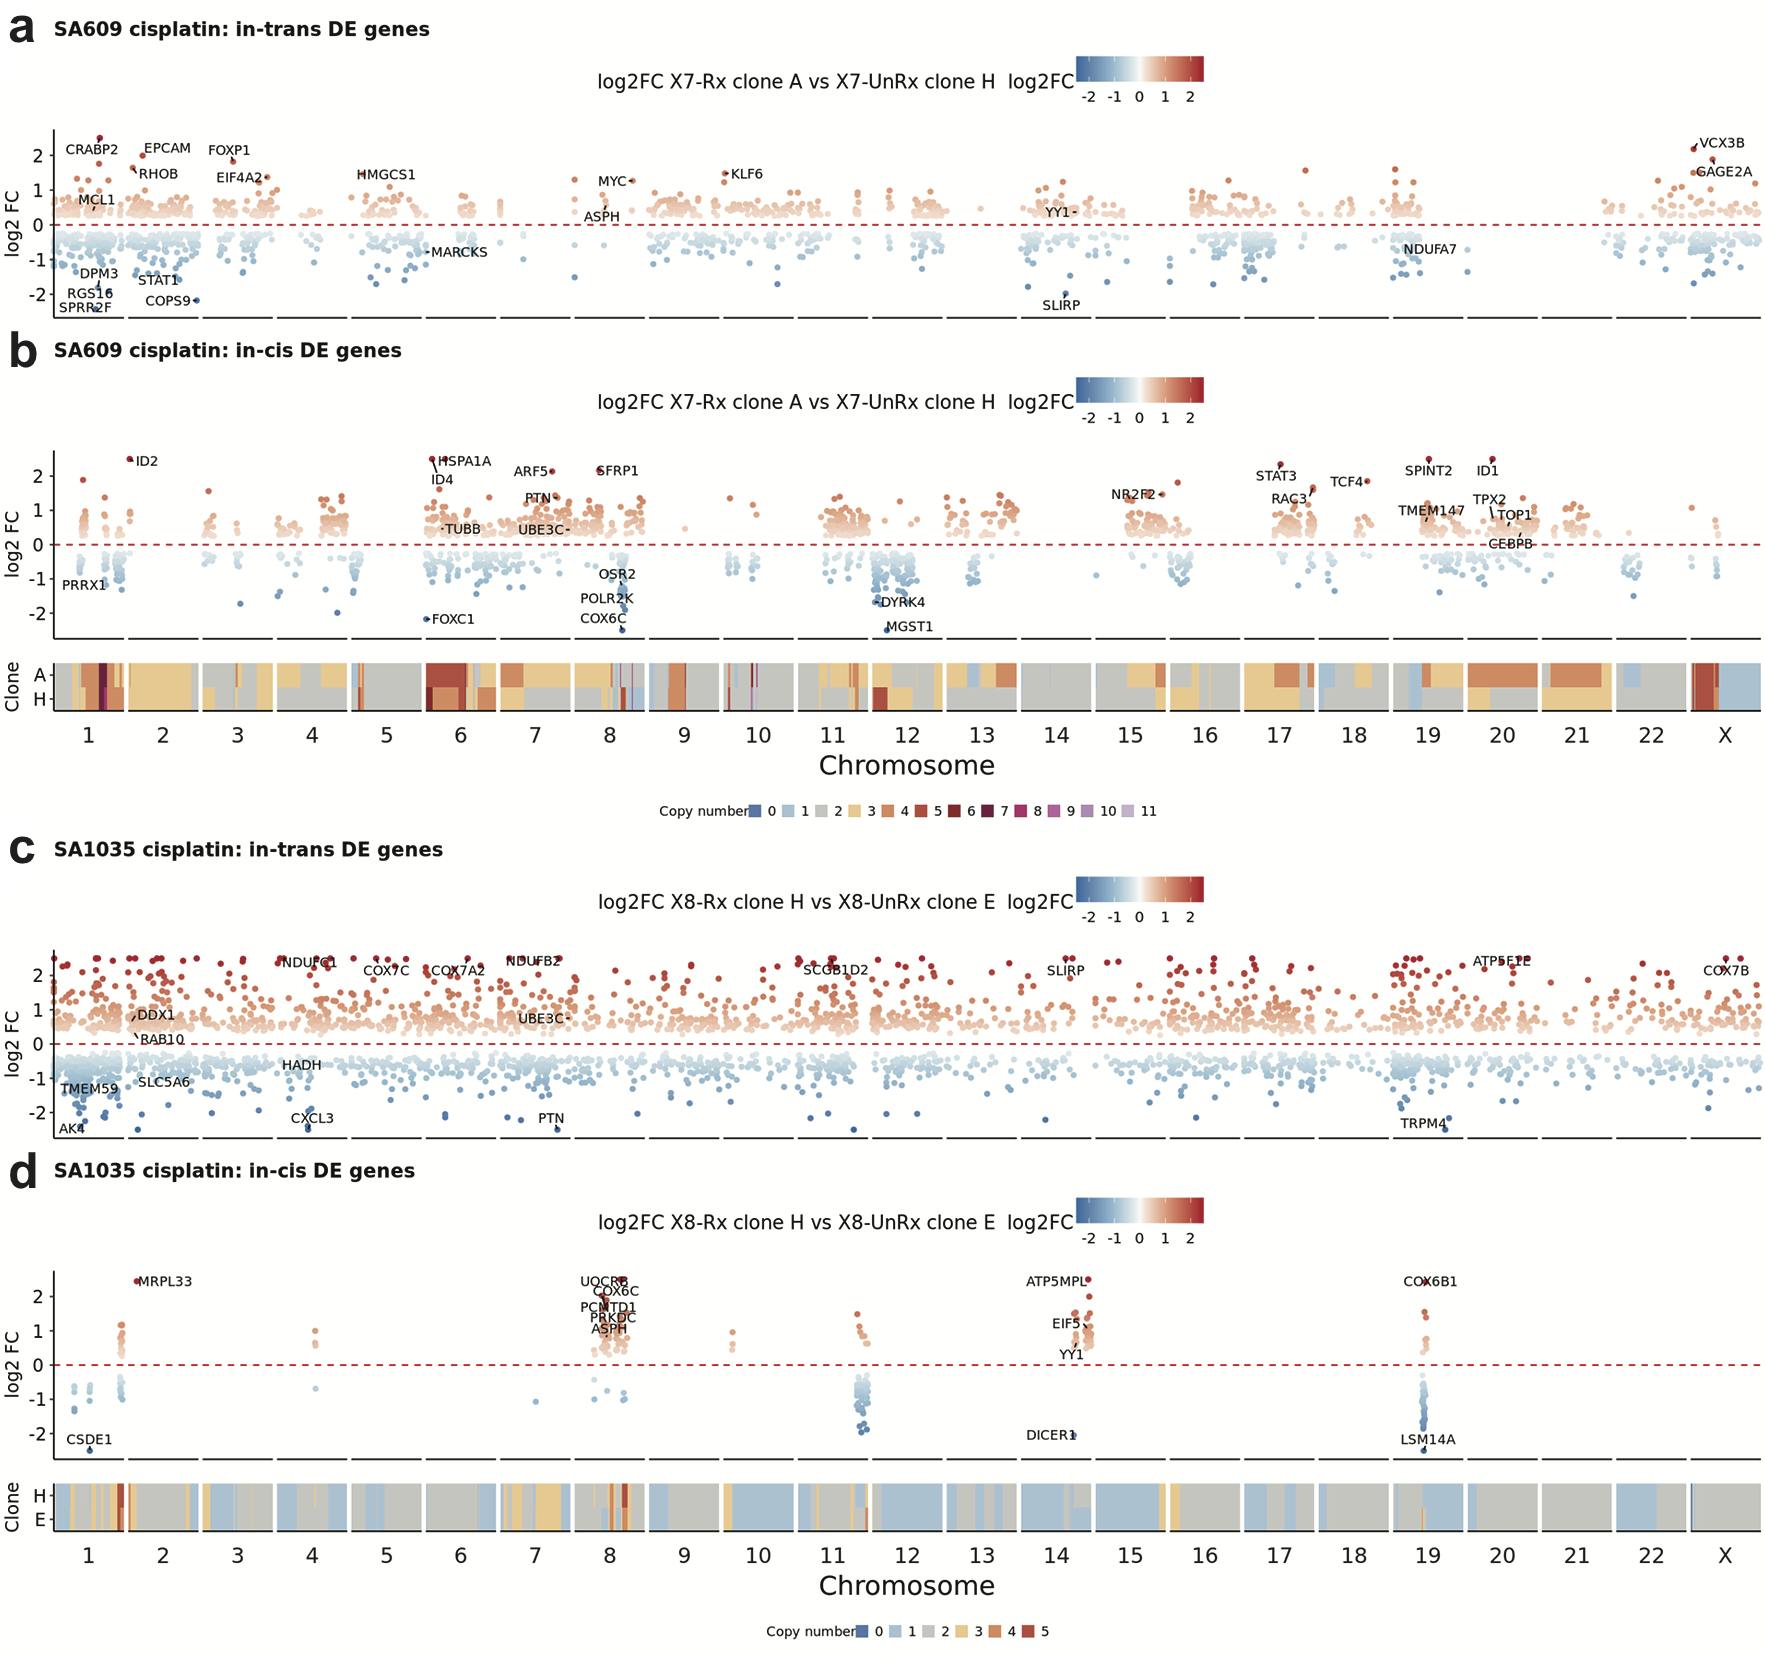
\includegraphics[width=\textwidth]{Figures/chap5/trackplotsSA609SA1035.png}
\caption[DE of resistant and sensitive \texttt{clonealign} defined clones]
	{\small
	\textbf{Differential expression of resistant and sensitive clones in TNBC-SA609 and TNBC-SA1035.}
 In each panel, the upper portion shows $\log 2$ fold change, with red colour showing higher log fold change in the top clone and blue showing higher log fold change in the bottom clone. All upper panel shows Manhattan plots of \textit{in trans} DEG, middle panel shows \textit{in cis}, bottom panel shows the median copy number of each gene from the DLP+ data, in the rank order of appearance in the genome.
 The percentage of \textit{in-cis} differentially expressed genes (DEGs) is calculated as having a corresponding change in copy number, out of all the DEGs considered. Red arrows in the middle panel highlighting important genes changing with change in copy number whereas, highlighting cancer related genes in upper \textit{in trans} DEG panel. 
 \textbf{(a)} Upper panel shows Manhattan plots of \textit{in trans} DEG, middle panel shows \textit{in cis}, bottom panel shows the median copy number of each gene from the DLP+ data, in the rank order of appearance in the genome in TNBC-SA609.
 \textbf{(b)} Same as \textbf{a} but in TNBC-SA1035.
}
	\label{fig:trackplotsSA609SA1035}
 \end{figure}

%------------------------------------------------------------
\begin{figure}
\centering
  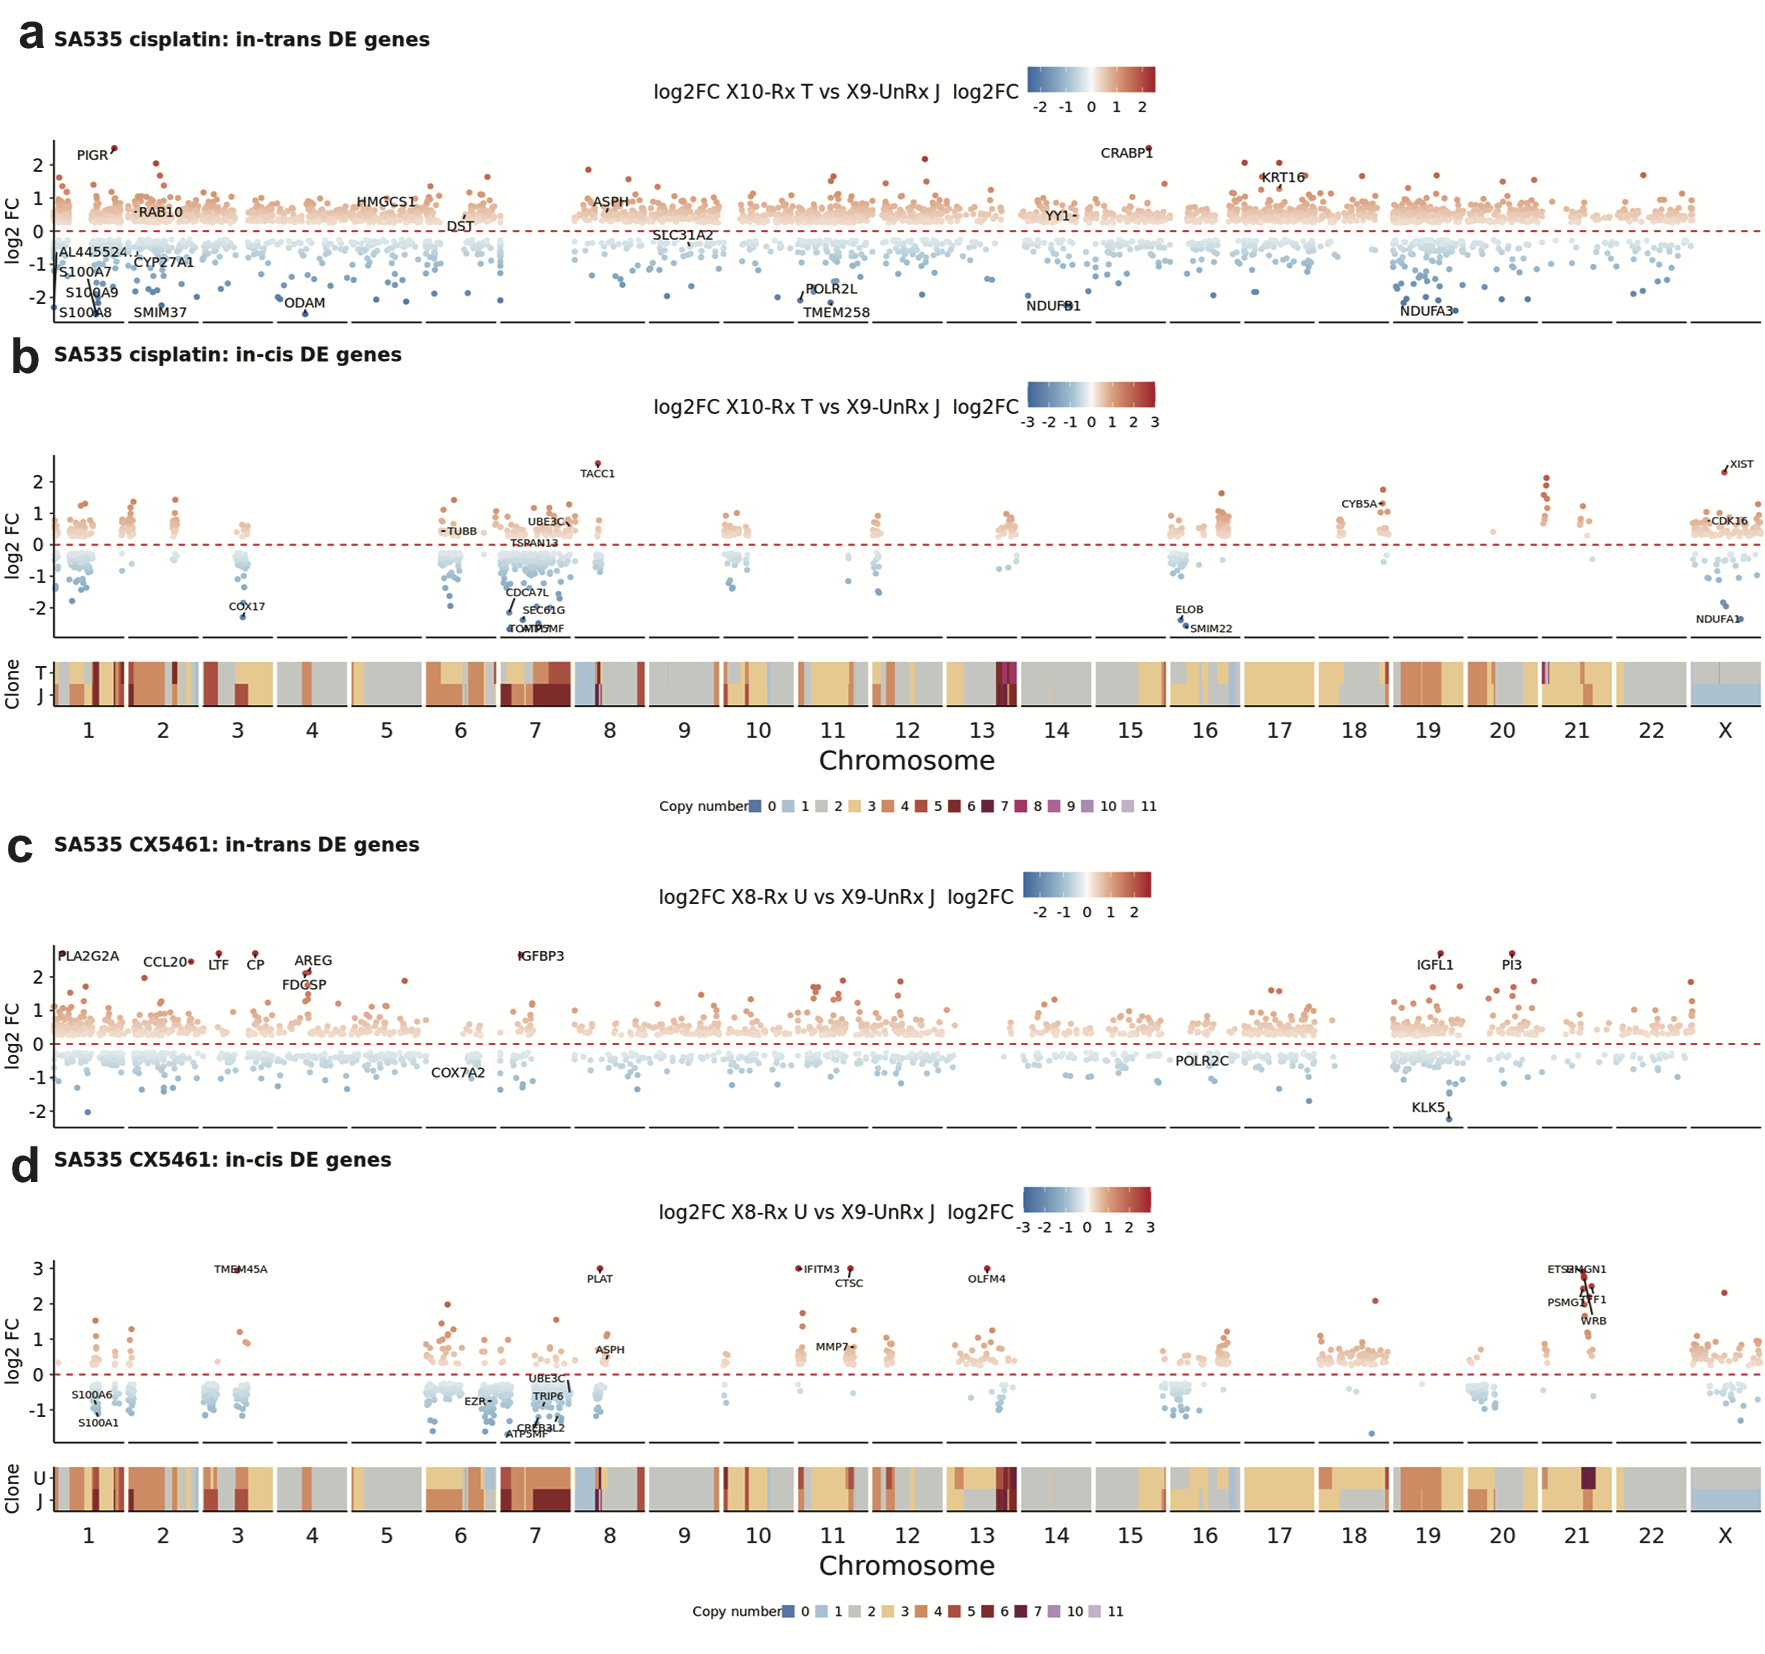
\includegraphics[width=\textwidth]{Figures/chap5/trackplotsSA535.png}
\caption[DE of resistant and sensitive \texttt{clonealign} defined clones]
	{\small
	\textbf{Differential expression of resistant and sensitive clones in TNBC-SA535 treated with cisplatin and CX5461.}
 In each panel, the upper portion shows $\log 2$ fold change, with red colour showing higher log fold change in the top clone and blue showing higher log fold change in the bottom clone. All upper panel shows Manhattan plots of \textit{in trans} DEG, middle panel shows \textit{in cis}, bottom panel shows the median copy number of each gene from the DLP+ data, in the rank order of appearance in the genome.
 The percentage of \textit{in-cis} differentially expressed genes (DEGs) is calculated as having a corresponding change in copy number, out of all the DEGs considered. Red arrows in the middle panel highlighting important genes changing with change in copy number whereas, highlighting cancer related genes in upper \textit{in trans} DEG panel.  
 \textbf{(a)} Upper panel shows Manhattan plots of \textit{in trans} DEG, middle panel shows \textit{in cis}, bottom panel shows the median copy number of each gene from the DLP+ data, in the rank order of appearance in the genome in in TNBC-SA535 traeted with cisplatin.
 \textbf{(b)} Same as  \textbf{a} but in TNBC-SA535 treated with CX-5461.
}
	\label{fig:trackplotsSA535}
 \end{figure}
%-----------------------------------------------------

\subsubsection{Differential expression analysis of resistant and sensitive clones reveals \textit{in cis} dynamics}

To explore the quantitative differences in expression between \textit{in cis} and \textit{in trans} regulation, I examined the relationship of differential expression between resistant and sensitive clones (\textbf{\autoref{fig:Volcanoes4plots}}, \textbf{\autoref{fig:trackplotsSA609SA1035}},  \textbf{\autoref{fig:trackplotsSA535})} and observed that the overall number of \textit{in trans} regulated genes were greater than \textit{in cis} number of genes, consistent with already established results.
\\
 I found that DE \textit{in cis} genes ranged from 6.9\% (SA1035-resH and senE) to 48.7\% (SA609-resA and senH) of all DE genes, for resistant vs sensitive clones. However, the proportion of DE \textit{in trans} genes ranged from- 44.12\% (SA609-resA vs senH) to  93.18\% (SA1035-resH and senE) and  72.2\% and  59.26\% for SA535 treated with cisplatin and CX5461, respectively.

Moreover, in top 5\% of the proportion of \ac{DE} of all datsets of resistant versus sensitive clones, the percentage of \textit{in trans} were higher than \textit{in cis} genes, except for series SA609, where \textit{in trans} almost balanced \textit{in cis} with the percentages of 44.12\% and 55.88\% respectively.

Next, I looked into the difference of magnitude between up regulated and downregulated \ac{DE} genes. Notably, all comparisons of the resistant versus sensitive clones showed approximately equal upregulated and downregulated gene sets except for SA535:Cisplatin treated resistant and sensitive comparison, that had around double the difference \textbf{(\autoref{fig:Volcanoes4plots} c)}.

The genomic landscape reflected copy number differences between resistant and sensitive clones and exhibited \textit{in cis} directional expression over the copy number interval, reflecting the impact of clone-specific copy number genotypes on transcription. 
Notably, positive linear tendency \textbf{(In cis Gain-Up)} of \textit{in cis} regulated DE genes were higher in all 4 timeseries datasets. SA609, had the highest number of \textbf{926 DE genes} that were upregulated with gain in copy number from sensitive to resistant clone \textbf{(\autoref{fig:Volcanoes4plots} a)}, for example, \textbf{ID4 and HSPA} were upregulated with copy number gain on \textbf{chromosome 6} \textbf{(\autoref{fig:trackplotsSA609SA1035} a) }. Similarly, in SA535, \textbf{XIST} had a copy gain on \textbf{chromosome X} and it was up regulated \textbf{(\autoref{fig:trackplotsSA535} a, b)}.
\\
SA609, also showed highest number of \textbf{214} DE genes that had negative tendency, meaning the DE gene was paradoxically regulated. With copy number gain, its downregulated \textbf{(In cis Gain-Down)}, for example, \textbf{FOXC1} gene on \textbf{chromosome 6} was downregulated with a copy number gain from sensitive to resistant clone \textbf{(\autoref{fig:trackplotsSA609SA1035} a) }.
\\
SA535:CX5461 had the highest number of \textbf{697} DE genes that were downregulated with copy number loss \textbf{(in cis Loss-Down)}, from sensitive to resistant clone \textbf{(\autoref{fig:Volcanoes4plots} d)}, for example, for example, \textbf{UBE3C, TRIP6, CREB3L2 and ATP5MF} were downregulated along with copy number loss on \textbf{chromosome 7} \textbf{(\autoref{fig:trackplotsSA535} b)}.
\\
SA1035 showed the highest number of \textbf{271} DE genes that were upregulated with copy number loss \textbf{(In cis Loss-Up)}, for example, \textbf{COX6B1} gene on \textbf{chromosome 19} was upregulated even there was a copy number loss from sensitive to resistant clone \textbf{(\autoref{fig:trackplotsSA609SA1035} b)}. Similarly, in SA609 \textbf{MYC} gene on \textbf{chromosome 8} was up-regulated even though had a copy number loss \textbf{(\autoref{fig:trackplotsSA609SA1035} a) }.


%------------------------------------------------------------
 %\begin{figure}
%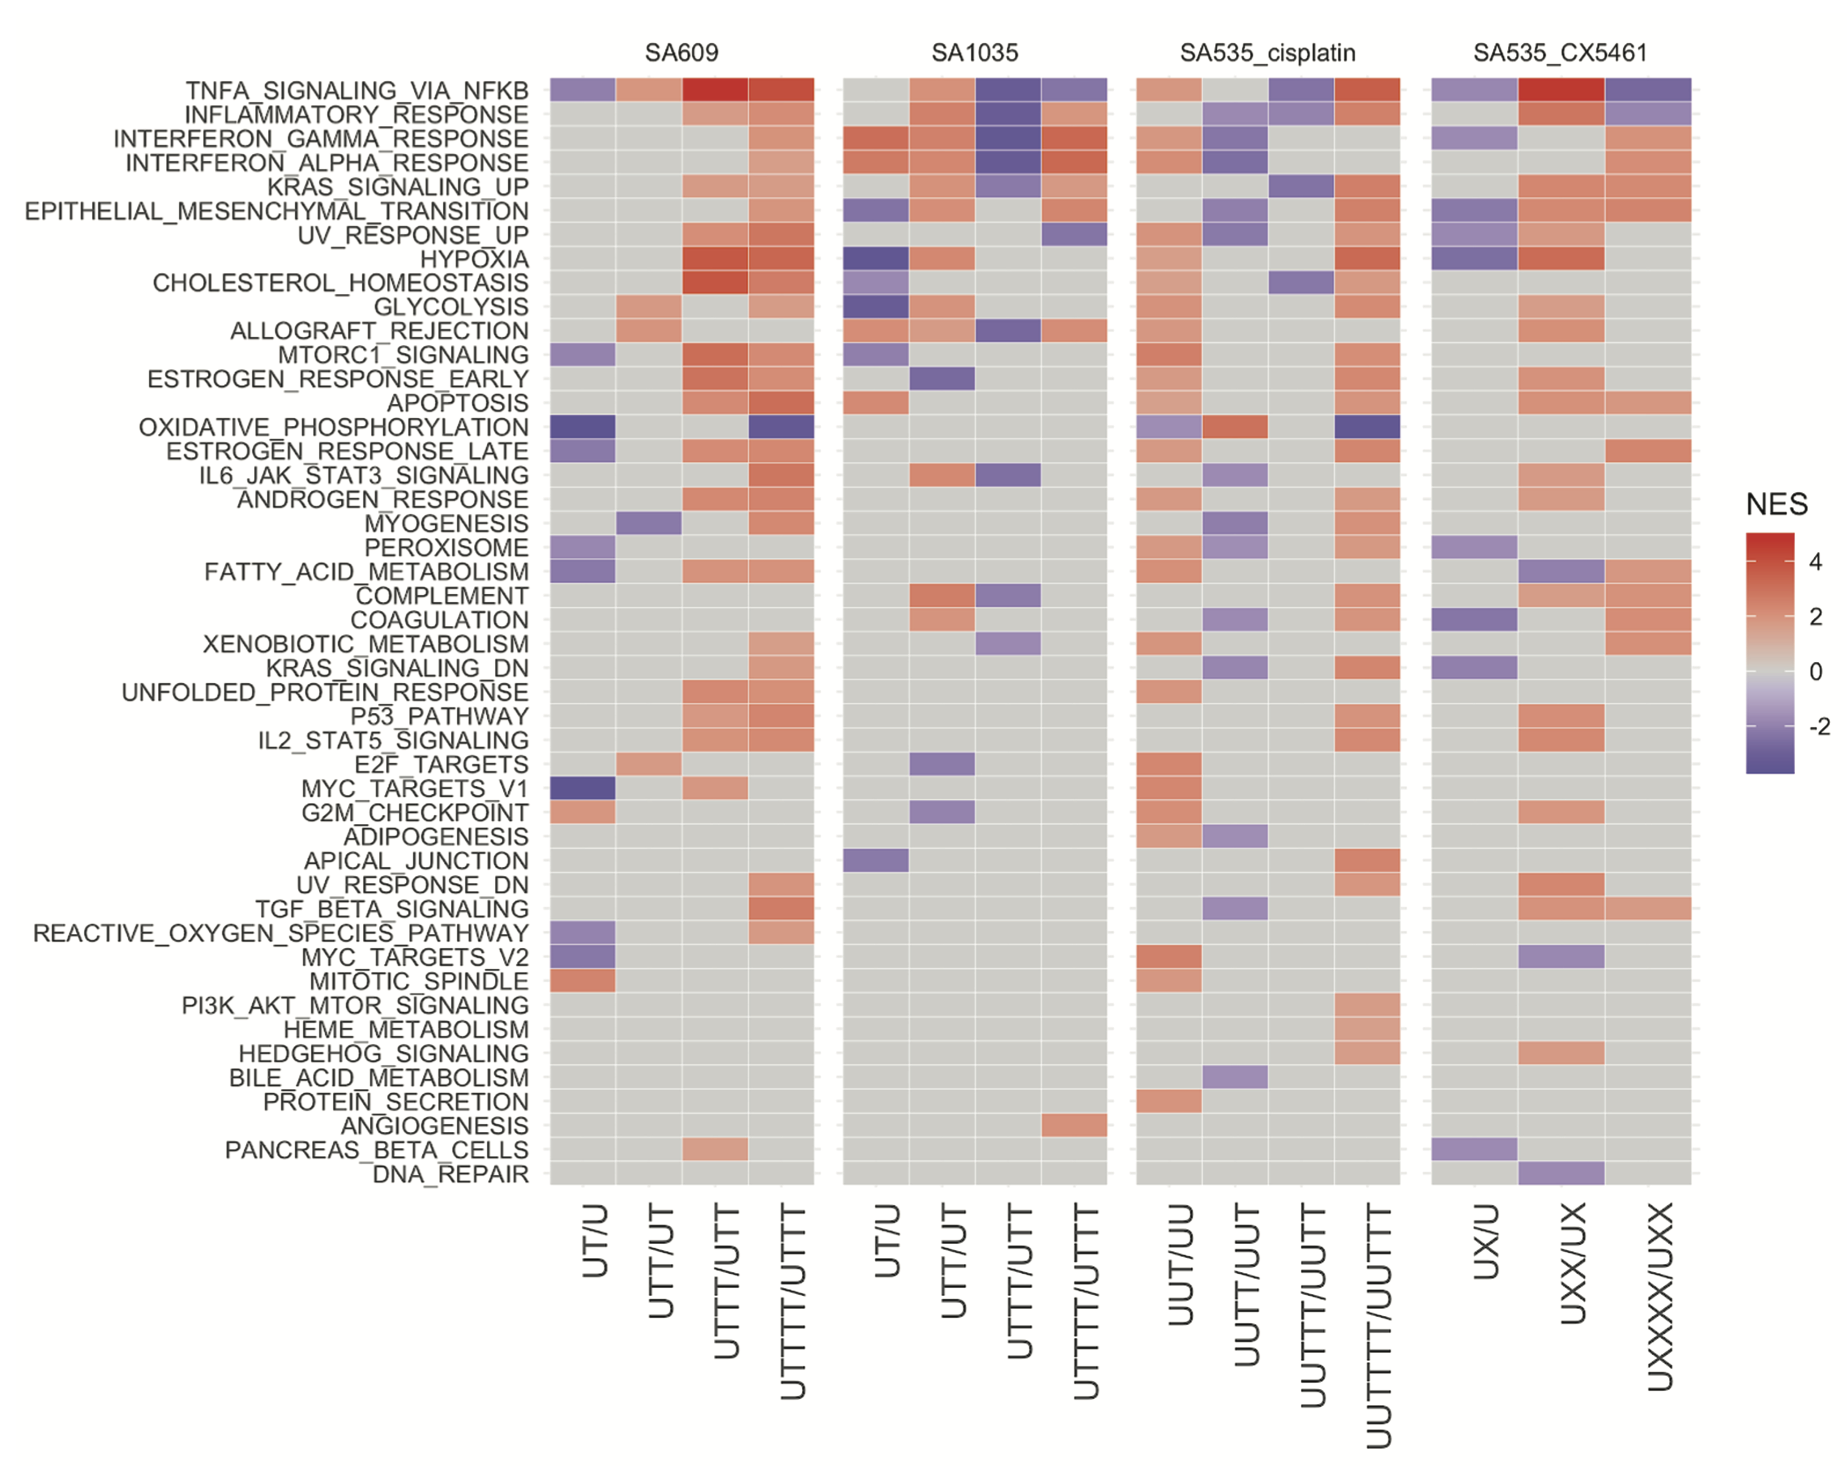
\includegraphics[width=\textwidth]{Figures/chap5/pathwaysevolution.png}
%\caption[Summary of number of genes \textit{in-cis} and \textit{in-trans}]
%	{\small
%	\textbf{Pathways comparison over time under chemotherapy in all PDX series}
%	Vertical left column enlist the pathways analysed. Horizontal axis at the bottom, represents the comparisons made between the time points and the treatment status. each single `T' indicates the number of cycles of the treatment from cisplatin. Each `X' indicates number of cycles of CX-5461 treatment. Colour intensity identifies normalized enrichment score (NES). Horizontal axis on top denotes the IDs of TNBC PDX. A normalized enrichment score (NES) was calculated from a ranked gene set enrichment analysis (GSEA) \cite{shi2007gene} performed on each subset of differentially expressed genes using the hallmark gene set collection from MSigDB \cite{liberzon2015molecular}.  Significantly enriched pathways (adjusted p-value $<$ 0.01).
%}
 %   \label{fig:pathwaysevolution}
%    \end{figure}
%-------------------------------------------------------------------
\begin{figure}
\centering
  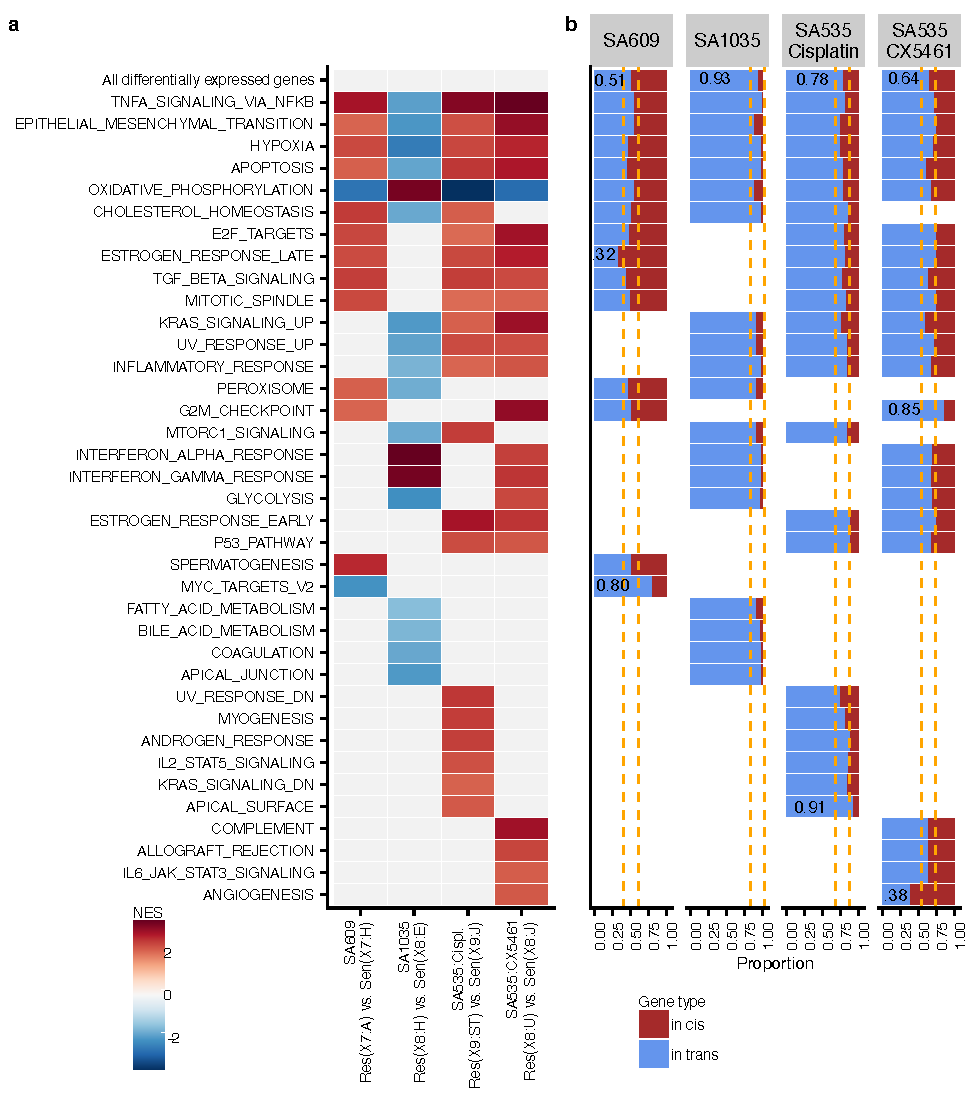
\includegraphics[width=\textwidth]{Figures/chap5/fig13_common_pathways.pdf}
\caption[Gene pathway enrichment analysis of PDX timeseries]
	{\small
	\textbf{Significantly enriched pathways with proportions of \textit{in cis} and  \textit{ in trans} regulated genes} ($p < 0.05$, vertical axis) from a ranked gene set enrichment analysis (GSEA) \cite{shi2007gene}, using the hallmark gene set collection from MSigDB \cite{liberzon2015molecular}. \textbf{(a)} Horizontal axis denotes the IDs of TNBC PDX and clones. Colour intensity identifies normalized enrichment score (NES) obtained by using all the differentially expressed genes at the specified time points and clones at FDR $< 0.01$. \textbf{(b)} \textit{In cis} (red) and \textit{in trans} (blue) gene proportions for each case depicted in panel \textbf{a}. Vertical dashed lines show the expected proportions (defined as the proportions of all differentially expressed genes, top row) plus or minus 10\%. The cases that are outside of the expected range are marked by the \textit{in trans} proportion numbers.
	}
	\label{fig:pathwaysnetworkcistrans}
\end{figure}


%-------------------------------------------------------------
\begin{figure}
\centering
  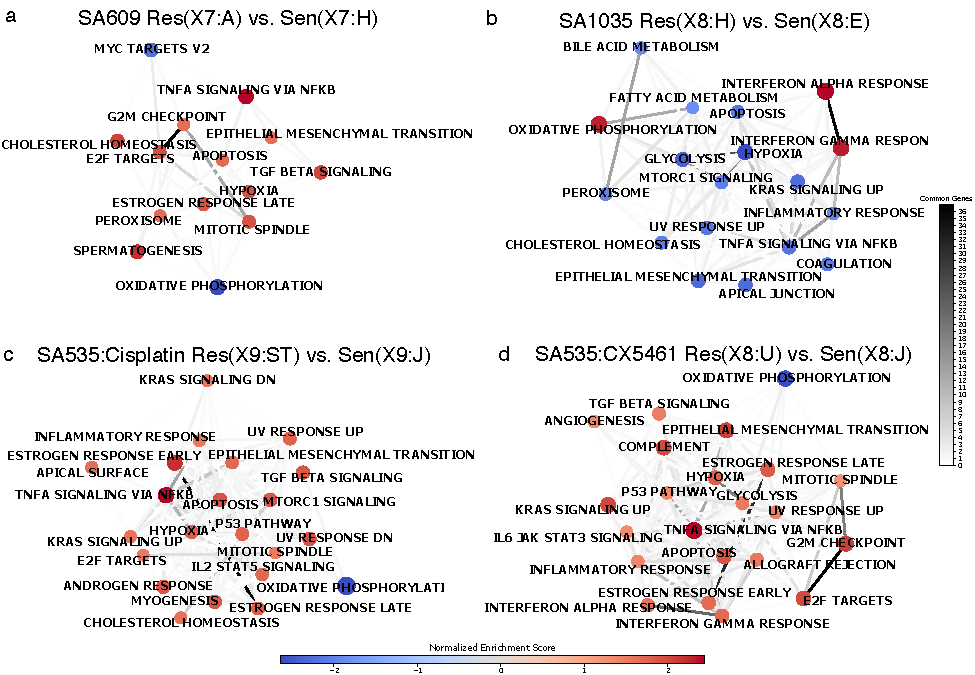
\includegraphics[width=\textwidth]{Figures/chap5/fig14_networks.pdf}
\caption[Gene pathway relationships of PDX timeseries]
	{\small
	\textbf{Networks showing the relationship between the enriched pathways in \textbf{\autoref{fig:pathwaysnetworkcistrans}}}. The color intensity denotes the normalized enrichment score (NES). The grey to black lines indicate the number of genes shared between pathways. (EMT: Epithelial Mesenchymal Transition;  OXPHOS:Oxidative Phosphorylation). \textbf{(a)} TNBC-SA609. \textbf{(b)} TNBC-SA1035.  \textbf{(c)} TNBC-SA535:Cisplatin. \textbf{(d)} TNBC-SA535:CX5461.
	}
	\label{fig:networks}
\end{figure}

%-------------------------------------------------------


%\subsection{Integrated transcriptome and pathway analyses revealed potential genes and key activated pathways in breast cancer}
%Next, I performed gene set enrichment analysis (GSEA) to search for sets of genes that are significantly over-represented in a given list of genes, compared to a background set of genes and their respective pathways and network connections. 
%First, I generated a heatmap of pathway evolution from one treated time point to another in all timeseries TNBC PDX \textbf{\autoref{fig:pathwaysevolution}}. Most of the listed pathways were enriched at the later timepoints, where tumours started developing chemoresistance. 

%\subsubsection{Profiling of signaling pathways reveals a distinct demarcation between SA1035 and rest of 3 TNBC PDX}
\subsubsection{Integrated transcriptome analyses revealed  activated pathways and \textit{in cis} proportions}
To assess the common pathways and their respective  \textit{in cis} gene  proportions, I profiled pathway enrichment scores between the resistant and sensitive clones of all TNBC PDX at the late time points. For TNBC-SA609 was X7 , X8 for TNBC-SA1035, X9 for TNBC-SA535:Cisplatin and X8 for TNBC-SA535:CX5461 (\textbf{\autoref{fig:pathwaysnetworkcistrans} a}, \textbf{\autoref{fig:networks}}). 


%Pathway specific differentially expressed genes were included in network enrichment analysis and the nodes were coloured by the normalized enrichment score (NES). 

Three PDX timeseries (TNBC-SA609, TNBC-SA535:Cisplatin, TNBC-SA535:CX5461) shared \textbf{8} common \textbf{upregulated pathways}, including:
\\
\textbf{TNFA signaling via NF-$\kappa$B}, including cisplatin resistance related such as, \textit{in cis} regulated DE:
ID2, FOS, NFKBIA, SAT1, BIRC2, DUSP1;
\\
\textbf{Epithelial mesenchymal transition (EMT)} such as, \textit{in cis} regulated DE: VCAN, CXCL8, CXCL6; 
\\
\textbf{TGF Beta signaling} such as, \textit{in cis} regulated DE: ID1, ID2, MAP3K7; 
\\
\textbf{Hypoxia} such as, \textit{in cis} regulated DE: MAFF, GAPDH, EGFR, HSPA, DUSP1;
\\
\textbf{Apoptosis} such as, \textit{in cis} regulated DE: TXNIP (downregulated tumour suppressor gene), TOP2A, HMGB, BRCA1, CASP3, MGMT, CCND2, ROCK1;
\\
 \textbf{E2F Targets} such as, \textit{in cis} regulated DE: POLE, MCM2, HMGB2, MLH1, BRCA2; 
 \\
 \textbf{Mitotic spindle} such as, \textit{in cis} regulated DE: BIRC5, TOP2A, MAP3K11, BRCA2, NOTCH2, BCL2L11, BUB1, AURKA, RASA1, PLK1;
 \\
 \textbf{Estrogen response} such as, \textit{in cis} regulated DE: S100A9, NBL1, TOP2A.
 \\ However, \textbf{Peroxisome} (specific to SA609) had \textit{in cis} regulated DE, such as: CRABP2, FIS1;IDI1, TSPO, TOP2A, ACAA1, PRDX5, IDH2. 
 \\\textbf{G2M\_CHECKPOINT pathways} (specific to SA609) \textit{in cis} regulated DE: CDKN2C, UBE2, MARCKS, MCM6, MAPK, CASP.
 
 On the other hand, only \textbf{OXPHOS pathway} was commonly downregulated in these three PDX series \textbf{(\autoref{fig:pathwaysnetworkcistrans} a}, \textbf{\autoref{fig:networks} a, c, d)}. However, SA1035 again showed distinct dynamics with only three upregulated pathways in resistant versus sensitive clones, including \textbf{Oxidative phosphorylation (OXPHOS)} such as, \textit{in cis} regulated DE: MRP, NDUFB2, BAX, ATP5F1E, COX7A2L, UQCRC1 (oncogenic); 
\textbf{Interferon alpha response} and \textbf{Interferon gamma response}. 
\\
Eight pathways were downregulated that were activated in other series (\textbf{\autoref{fig:pathwaysnetworkcistrans} a}, second column  \textbf{\autoref{fig:networks} b)}. 
 
Furthermore, $\sim$~40\% of the pathways (including \textbf{UV response, IL-2\_STAT5 signaling, KRAS, Apical surface, IL6\_JAK\_STAT3 signaling and Angiogenesis})  were unique to either tumour or drug condition. 

Cisplatin and CX5461 treated SA535 shared \textbf{11 upregulated pathways} and only one pathway, namely \textbf{\ac{OXPHOS}}, was down regulated in both series, suggesting their specificity to the tumour.

% those numbers are over all genes, not over pathway genes
%Overall, $\sim$~50\% \textit{in cis} genes were in upregulated pathways of TNBC-SA609 consistent with the previous proportions. However, TNBC-SA1035 remained the highest PDX in containing \textit{in trans} proportion (0.93) of genes in the pathways. 

Finally, the proportions of \textit{in cis} and \textit{in trans} genes in the gene set enrichment pathways largely mirrored the proportion in the entire population of genes for most pathways, with only a few exceptions. In TNBC-SA609 (expected \textit{in trans} proportion 0.51), \textbf{Estrogen response late} pathway had a lower percentage of \textit{in trans} genes (0.32), while \textbf{MYC targets V2} had a higher percentage of \textit{in trans} genes (0.79). In TNBC-SA1035 all pathway proportions were within the expected range (0.93 \textit{in trans} proportion). In TNBC-SA535:Cisplatin (expected \textit{in trans} proportion 0.78), only \textbf{Apical surface} pathway had a higher \textit{in trans} proportion of 0.91. Finally, in TNBC-SA535:CX5461 (expected \textit{in trans} proportion 0.78), \textbf{EMT} and \textbf{G2M checkpoint} pathways had a higher \textit{in trans} proportion (0.76 and 0.85, respectively), and \textbf{Angiogenesis} had a lower \textit{in trans} proportion of 0.43. (\textbf{\autoref{fig:pathwaysnetworkcistrans} b)}.


%-----------------------------------------------------------------
\begin{figure}
\centering
 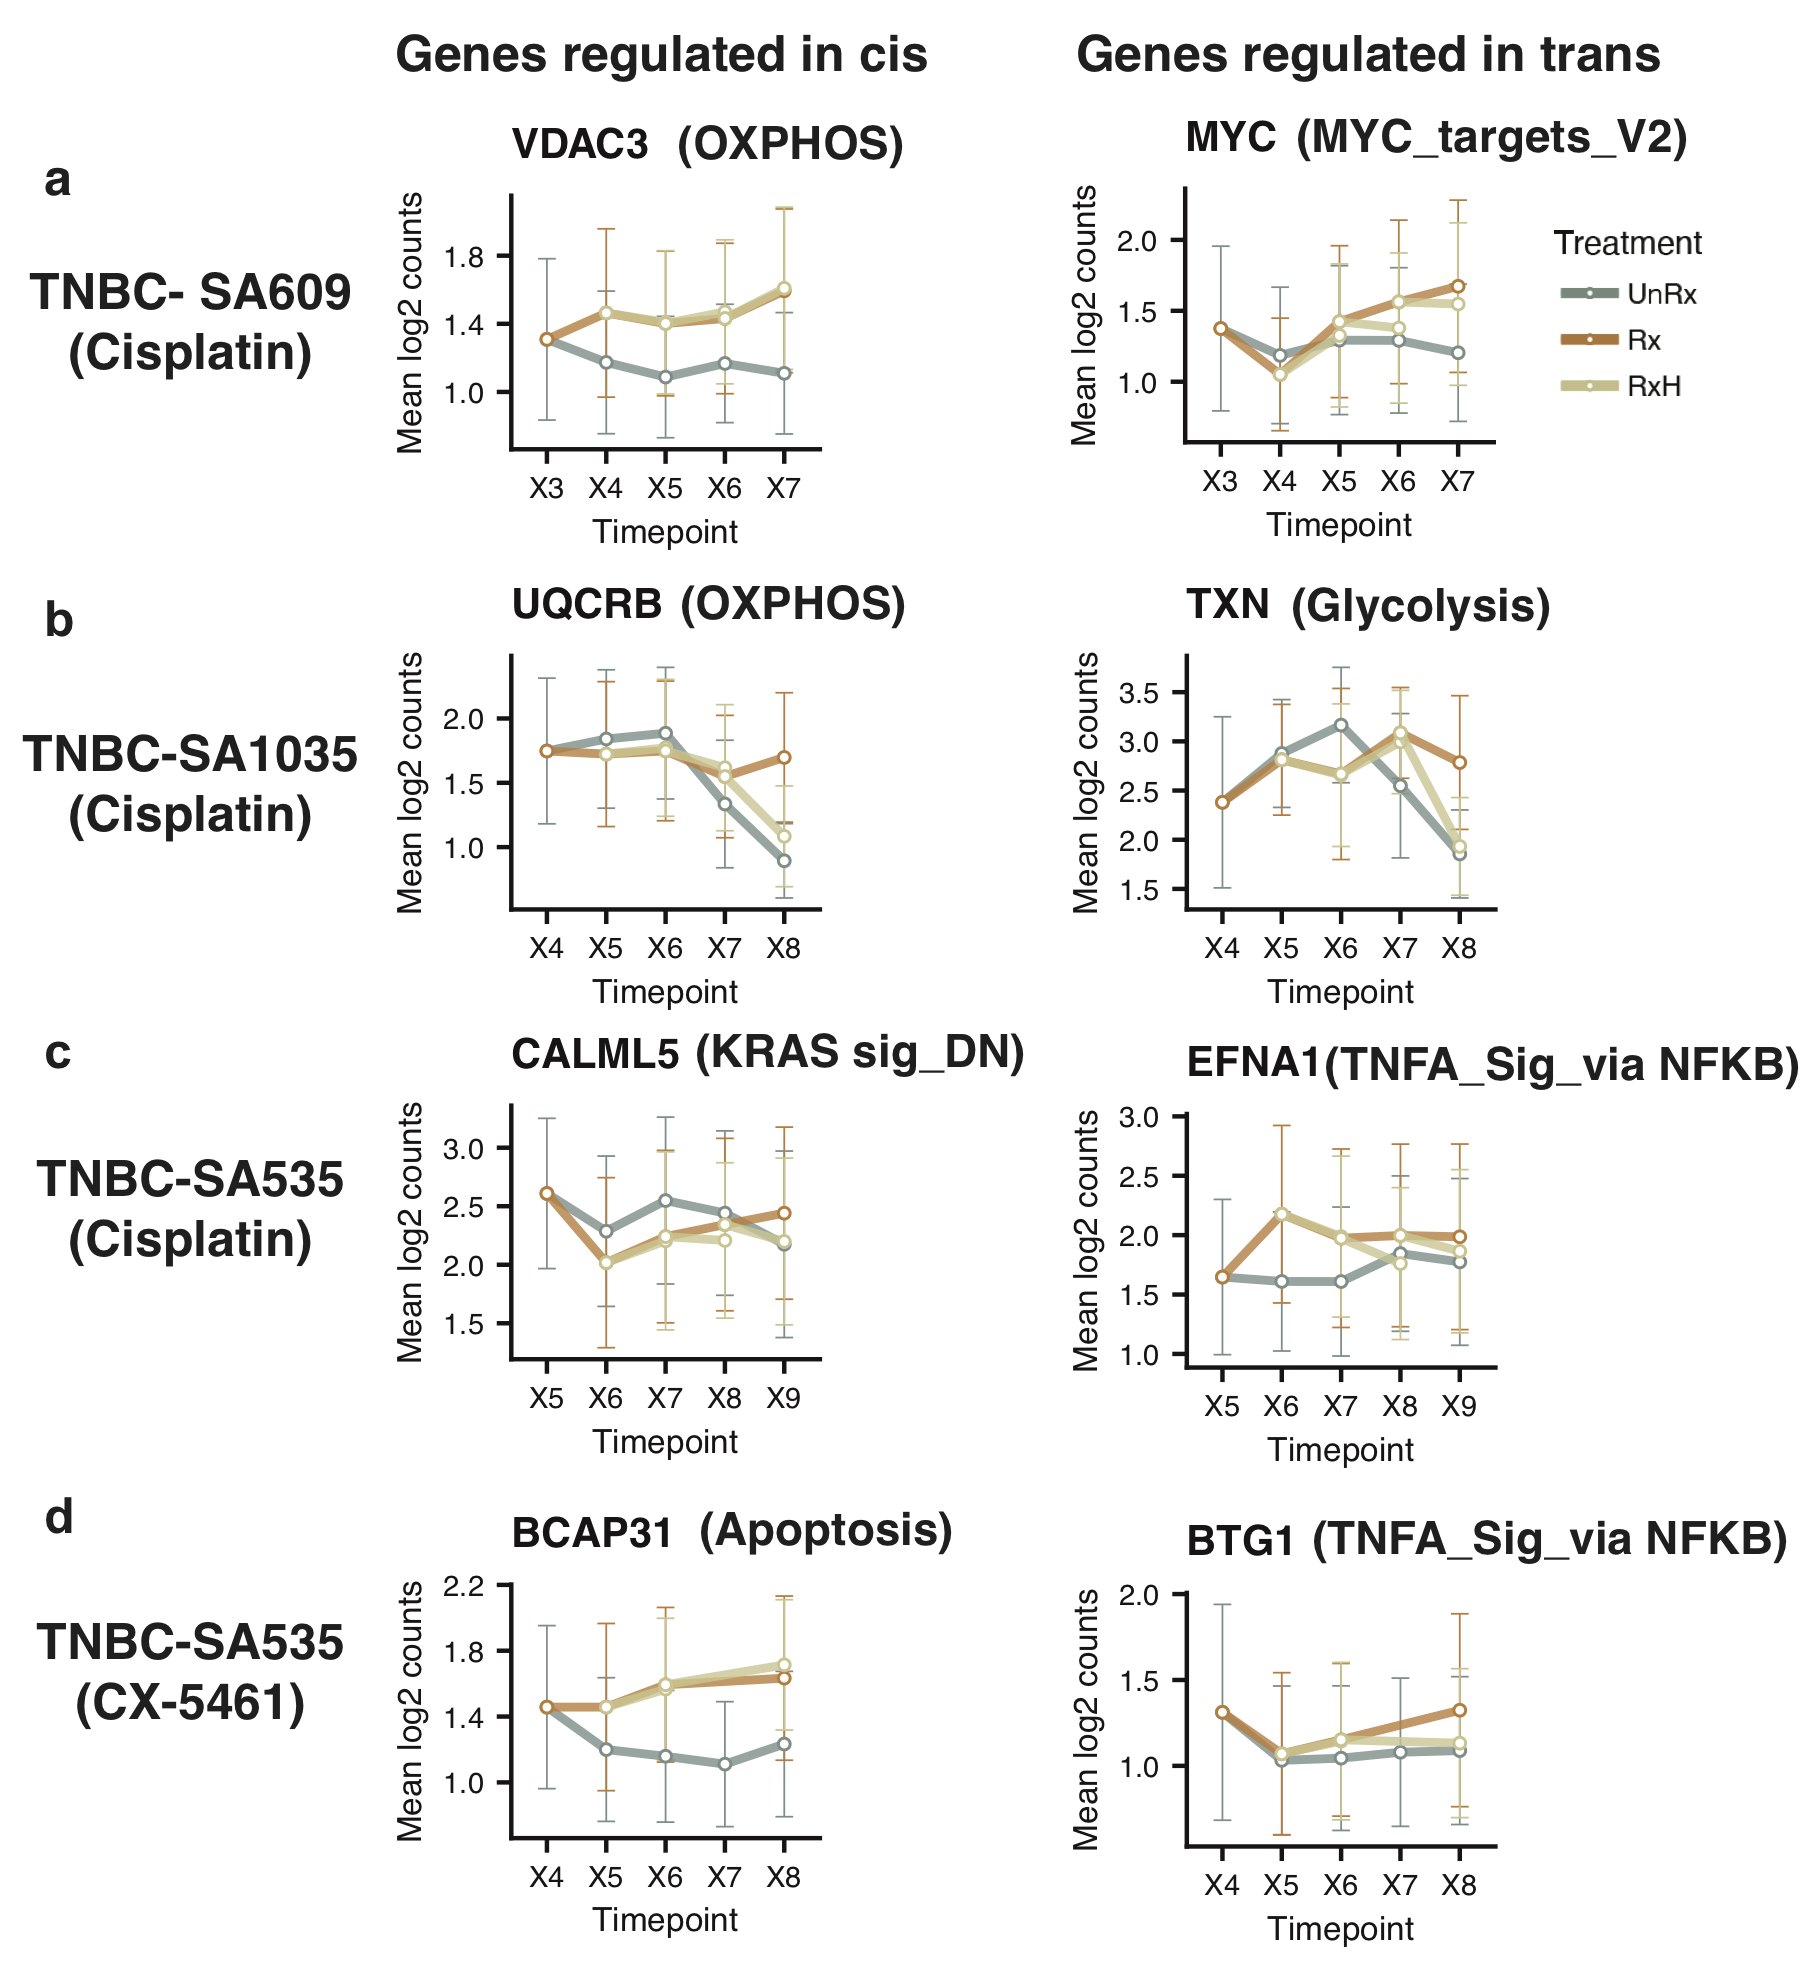
\includegraphics{Figures/chap5/fig16_lineplotscistrans.png}
\caption[Examples of \textit{in cis} and \textit{in trans} genes]
	{\small
	 \textbf{Time dependent dynamics \textit{in cis} and \textit{in trans} genes}.
	 Vertical axes represent mean log2 counts of expression while horizontal axes represent timepoints (passages). UnRx: Untreated, Rx: Treated, RxH: Drug holiday tumour. \textbf{(a)} Examples of \textit{in cis} and \textit{in trans} genes showing time dependent change in expression from SA609 from treated, untreated and drug holiday tumours.  \textbf{(b)} Analogous to \textbf{a} but for SA1035. \textbf{(c, d)} Analogous to \textbf{a} but for SA535:Cisplatin and CX-5461.}

	\label{fig:cistrans}
\end{figure}
%----------------------------------------------------------------

%Finally, I concluded that proportional contribution of \textit{in cis} and \textit{in trans} to pathways largely mirror that of the expected fraction from the copy number genome. Exceptions included  \textbf{Estrogen response late} in SA609 (larger \textit{in cis} proportion), \textbf{MYC Targets V2} in SA609 (larger \textit{in trans} proportion), \textbf{Apical surface} in SA535:Cisplatin (larger \textit{in trans} proportion), \textbf{G2M checkpoint} in SA535:CX5461 (larger \textit{in trans} proportion) and \textbf{Angiogenesis} in SA535:CX5461 (larger \textit{in cis} proportion).

%%%%%%%%%%%%%%%%%%%%%%%%%%%%%%%%%%%%%%%%%%%%%%%%%%%%%%%%%%%%%%%%%%%%%%%%%%
%-------------------------------------------------------
\begin{figure}
\centering
 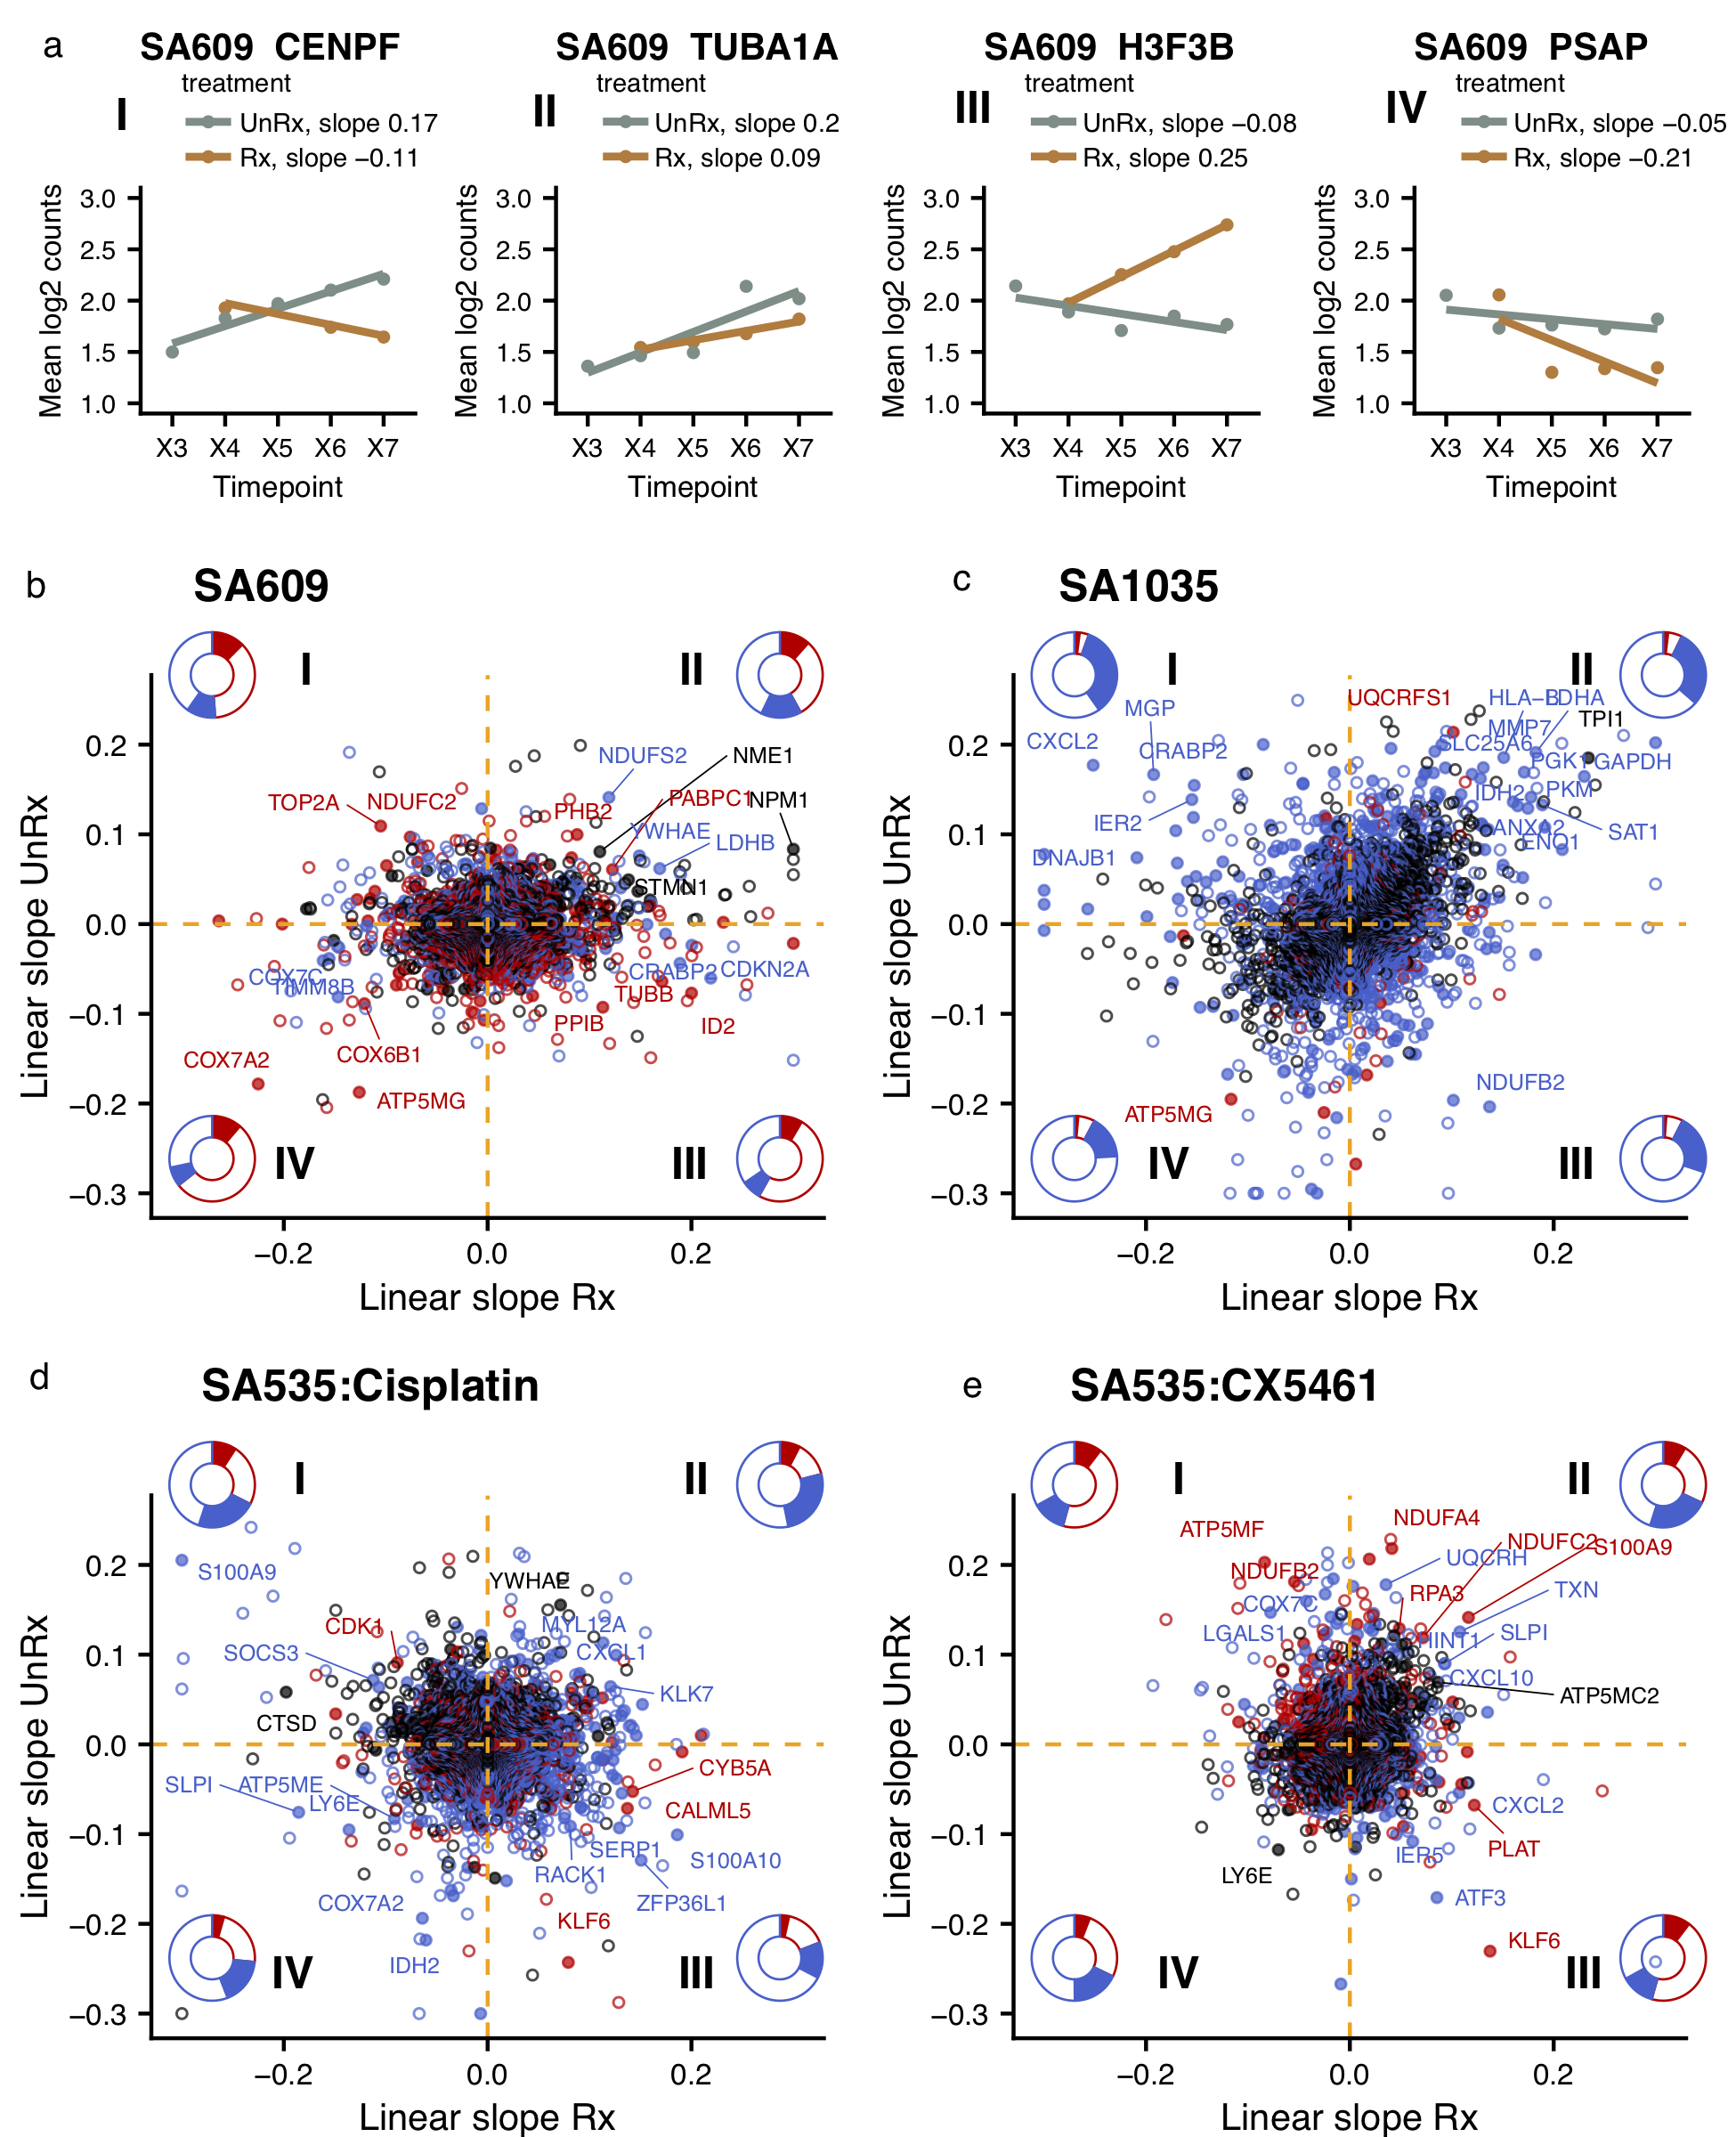
\includegraphics[width=\textwidth]{Figures/chap5/fig15_GeneschanginginRxclouds.png}
\caption{Gene expression changes over time with and without treatment in all 4 TNBC PDX timeseries.}% First caption
	\label{fig:GeneschanginginRxclouds}
\end{figure}
\begin{figure}[t]	
\contcaption
	{\small
\textbf{(a)} Examples of linear model fitting to mean log2 normalized gene expression at Rx and UnRx time points. \textbf{(b)-(e)} Scatter plots of linear slopes. Horizontal axis: Gene expression change with Rx. Vertical axis: UnRx timepoints. Each of the four quadrants are numbered as I (genes increasing in UnRx, decreasing with Rx), II (increasing in both UnRx/Rx), III (increasing in Rx and decreasing in UnRx) and  IV (decreasing in both UnRx/Rx overtime). Orange circles present radius of slope 0.07, corresponding to an average change of 5\% at each time point. Pie plots show the number of genes in each category outside of the orange circle. red and blue filled portions represent \textit{in cis} and \textit{in trans} number of genes present in DE pathways while unfilled present others. \textbf{(b)} TNBC-SA609. \textbf{(c)} TNBC-SA1035. %Rx and UnRx X5 samples were eliminated from the slope calculation due to lower data quality. 
\textbf{(d)} TNBC-SA535:Cisplatin. \textbf{(e)} TNBC-SA535:CX5461.}


\end{figure}


%-------------------------------------------------------------------

\subsection{Gene expression changes over time}

%\subsubsection{Gene specific expression trajectories exemplified systematic response to sustained treatment}

Next, I asked  about time and passage dependent changes in treated and untreated tumours. Line trajectories of individual genes over time showed that expression change was monotonically increasing or decreasing under drug selection in some of the tumours, for example, in SA609, \textit{in cis} regulated \textbf{VDAC3, from OXPHOS pathways} and \textit{in trans} regulated \textbf{MYC from MYC targets V2} were found to be increasing with drug over time \textbf{(\autoref{fig:cistrans} a)}. 
Similarly, in SA1035, \textit{in cis} regulated \textbf{UQCRB, from OXPHOS pathways} and \textit{in trans} regulated \textbf{TXN from Glycolysis} were found to be increasing with drug over time \textbf{(\autoref{fig:cistrans} b)}. 

In SA535, \textit{in cis} regulated \textbf{CALML5, from KRAS sig\_DN} and \textit{in trans} regulated \textbf{EFNA from TNFA\_sig\_via NFKB} from cisplatin, however, \textit{in cis}, \textbf{BCAP31, from Apoptosis} and \textit{in trans}, \textbf{BTG1 from TNFA via NF-$\kappa$B pathway} were exemplified as increasing with time \textbf{(\autoref{fig:cistrans} c, d)}. 
To examine the reversibility of gene expression, drug holiday samples were explored. \textit{in trans} expression, some clear examples of reversibility were observed, such as \textbf{MYC, from MYC targets V2}, \textbf{EFNA, from TNFA signaling via NF-$\kappa$B} and \textbf{BTG1, from TNFA signaling via NF-$\kappa$B} showed a shift towards untreated line (\textbf{\autoref{fig:cistrans} a, c, d-right}). 
\\
The variation over time for \textit{in cis} was confounded by changing clonal proportions, which requires a clone-time dependent expression model that was out of scope of this dissertation.


Next, to examine systematically time dependent changes in gene expression, linear models were fitted to time-series samples \textbf{(linear model-lm in R, see methods)} between treated and untreated scRNA-seq data. 
Time dependent trends that were co-varying between treated and untreated appeared to be equal \textbf{\autoref{fig:GeneschanginginRxclouds}}. 
%The slope of the linear fitting signifies the overall magnitude of change from one time point to the next. Since the y axis was on a log2 scale, a slope of 1 means that, on average over time, the expression level doubled with every time point. Similarly, slopes 0.1 and 0.2 mean that, on average, the expression level increased by 7\% and 15\%, respectively, at every time point.
 % However, the proportion of correlated gene expression in each direction was colinear with the contribution of CNA differences between clones.
%Notably again, SA1035 had fewer \textit{in cis} differences and had a higher number of time correlated genes \textit{in trans}.
\\
The genes in quadrants II and IV were changed in the same direction in both treated and untreated (up in II and down in IV), suggesting dynamics due to passage, and not due to treatment status. Conversely, the genes in quadrants I and III changed in the opposite direction in the treated samples versus the untreated samples, suggesting dynamics due to treatment status. While the vast majority of genes form a "cloud" around the origin, a small number of genes fall outside of the radius of slope 0.07, corresponding to an average of 5\% from one time point to another. 

There was no significant difference between the distribution of \textit{in cis}/\textit{in trans}, all genes (in the pathways or not in the pathways) in counter time cases (quadrants I and III) versus those in coordinated time cases (quadrants II and IV), paired t-test: p>1.4, in all cases.
\\
All the quadrants were quite closer to each other within each series in terms of number of genes \textit{in cis} and \textit{in trans}.
Consistent with the previous results of proportions of differentially expressed genes \textit{in cis} and \textit{in trans}, SA609 showed the highest number of \textit{in cis} regulated genes in each of the four quadrants ranged from \textbf{22 (quadrant I-untreated increasing, treated decreasing)} to \textbf{36 (quadrant III-untreated decreasing, treated increasing)} DE genes present in the activated pathways, \textbf{32 (quadrant II-both increasing)} and \textbf{25 (quadrant IV-both decreasing)} \textit{in cis} in quadrants II and IV respectively, \textbf{\autoref{fig:GeneschanginginRxclouds} b}. However, the total number of \textit{in cis} regulated gene expression other than DE, was also highest in SA609, shown as red outlined portion of pie charts \textbf{(\autoref{fig:GeneschanginginRxclouds} b)}, ranged from \textbf{56 (quadrant I-untreated increasing, treated decreasing)} to \textbf{69 (quadrant III-untreated decreasing, treated increasing)} \textbf{\autoref{fig:GeneschanginginRxclouds} b-pie charts in all quadrants}.
\\
SA1035, possessed the highest number of \textit{in trans} genes in all quadrants, ranged from \textbf{88 (quadrant IV (both decreasing)} to \textbf{129 (quadrant II-both increasing)} and \textbf{135 (quadrant I-untreated increasing, treated decreasing)} and \textbf{105 (quadrant III-untreated decreasing, treated increasing)} in quadrants II and III, respectively \textbf{(\autoref{fig:GeneschanginginRxclouds} c)}. \textit{in cis} regulated gene expression changes over time in SA1035 was very small, ranged from \textbf{2 (quadrant II-both increasing)} to \textbf{6 (quadrant III-untreated decreasing, treated increasing, quadrant IV-both decreasing)}, \textbf{\autoref{fig:GeneschanginginRxclouds} c-pie charts in all quadrants} 
\\
SA535, in both treatment regimes were consistent in terms of \textit{in cis} and \textit{in trans}. SA535:Cisplatin had DE \textit{in cis} genes ranged from \textbf{4 (quadrant I-untreated increasing, treated decreasing)} to \textbf{19 (quadrant II-both increasing, quadrant III-untreated decreasing, treated increasing} \textbf{(\autoref{fig:GeneschanginginRxclouds} d)}. However, SA535:CX5461 had DE \textit{in cis} genes ranged from \textbf{7 quadrant IV-both decreasing)} to \textbf{23 (quadrant II-both increasing} \textbf{(\autoref{fig:GeneschanginginRxclouds} e)}.




%Genes in treated and untreated samples form specific direction of slope as examplified with SA609 genes with region numbers I (untreated increasing, treated decreasing), II (both increasing), III (untreated decreasing, treated increasing), IV (both decreasing), directions \textbf{\autoref{fig:GeneschanginginRxclouds} a}.
%\textbf{\autoref{fig:GeneschanginginRxclouds} b-e} show the untreated slope (y axis) versus the treated slope (x axis) for each gene in four series, with the \textit{in cis} and \textit{in trans} genes shown in red and blue colours, respectively.
%distribution of coefficients (between 13 and 202 genes).  

%--------------------------------------------------------------------------

\subsection{Temporally correlated expression highlight EMT, metabolic and cisplatin resistance pathways.}
 To understand the change in pathways activation with increasing cycles of drug, pathways evolution between resistant and sensitive clones were explored over time. Notably, pathway analysis over time points a gradual increase in pathway representation with increasing drug exposure, for example, \textbf{MYC targets V1 and V2} in SA609, were observed gradually increasing its normalized enrichment score (NES) from first cycle of cisplatin to last cycle of cisplatin (passage 4 to passage 7) \textbf{(\autoref{fig:pathwayevolution} dark blue to light blue)}. NES was obtained by using all the differentially expressed genes at the specified time points and clones at FDR $< 0.01$. 
 %NEScalculated by dividing positive and negative ES by the mean of positive or negative pES, respectively.
 
 However, \textbf{Epithelial mesenchymal transition (EMT) pathway} was found to be more activated from initial to late cycles of cisplatin in SA609, SA535 and SA535 treated with CX-5461 \textbf{(\autoref{fig:pathwayevolution} light red to dark red)}. \textbf{TGF-$\beta$ signaling}, a critical cellular initiator of EMT \cite{wellner2009emt}, was also found to be gradually increasing its activity over time. 

Some metabolic pathways, including \textbf{OXPHOS, Glycolysis, Peroxisome} were also found to be dominant at later time points and their direction were tumour type dependent.
 
 Similarly, \textbf{E2F targets}, in SA535, cisplatin treated, although remained activated but its NES was decreasing overtime \textbf{(\autoref{fig:pathwayevolution} dark red to light red)}. Main downregulated pathway in SA609 and SA535, \textbf{OXPHOS} also found to be more downreguated with decreasing NES \textbf{(\autoref{fig:pathwayevolution} light blue to dark blue)}.
 
Consistently, SA1035 remained unique by showing opposite but time dependent direction of pathways.
Most of the later time points, in the pathway analysis, exhibited significant activated pathways that were not activated at the initial time points. There was a strong representation of known cisplatin resistance pathways, such as \textbf{TNFA signaling via NF-$\kappa$B, EMT, signaling via NF-$\kappa$B, TGF beta signaling, MTORC1, IL-2\_STAT5 signaling, KRAS signaling down, Hypoxia and Apoptosis} \textbf{(\autoref{fig:pathwayevolution})} \cite{peng2010role, wu2020activation, gutierrez2020role, tao2014oncogenic, galluzzi2012molecular} \textbf{(also see introduction)}. 

\begin{figure}
\centering
 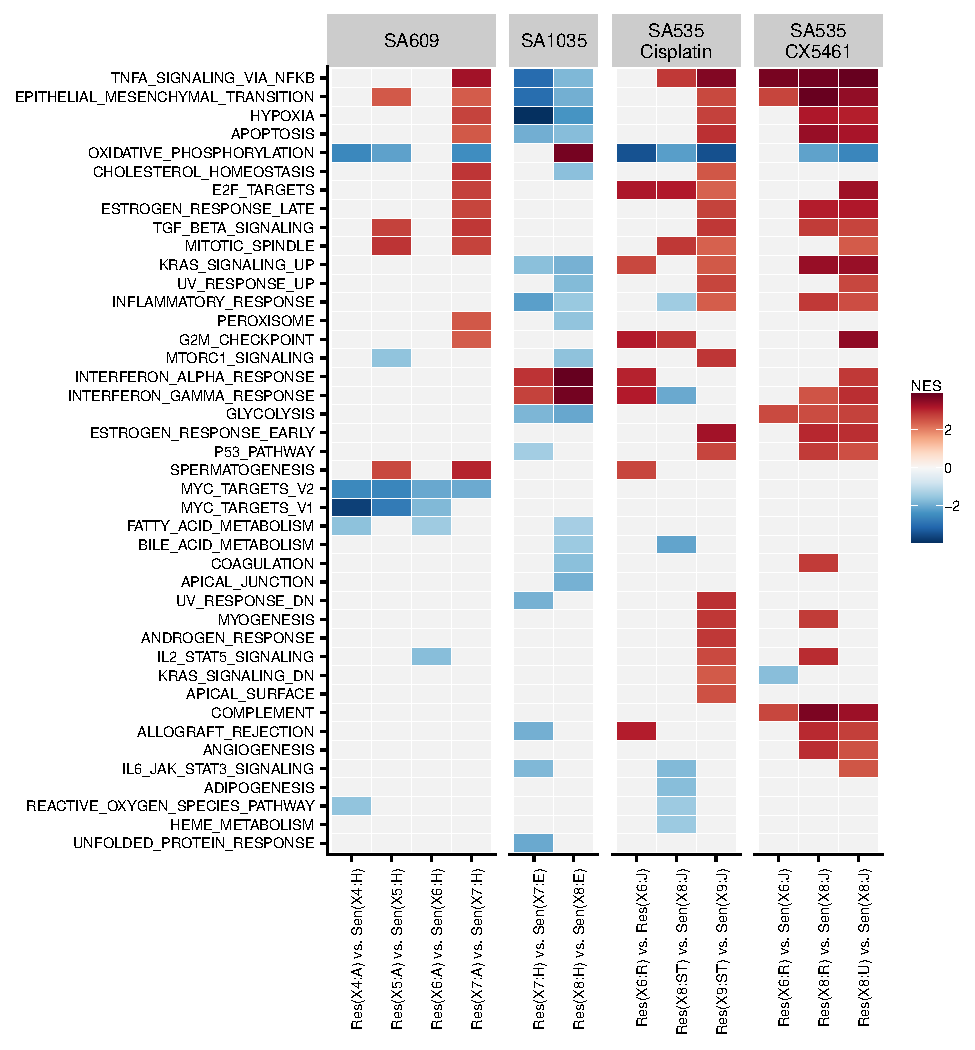
\includegraphics[width=\textwidth]{Figures/chap5/fig17_pathway_evolution.pdf}
\caption[Pathway evolution over passages]
	{\small
	 \textbf{Pathway evolution over passages}. GSEA pathway analysis similar to \textbf{\autoref{fig:pathwaysnetworkcistrans} a}, but here I also included earlier time points for each of the four TNBC PDX. For SA535, I also included the precursor resistant clone R at time point X6 for both cisplatin and CX5461, and at X8 for CX5461.
	 }

	\label{fig:pathwayevolution}
\end{figure}
%---------------------------------------------------------------------------

\begin{figure}
\centering
 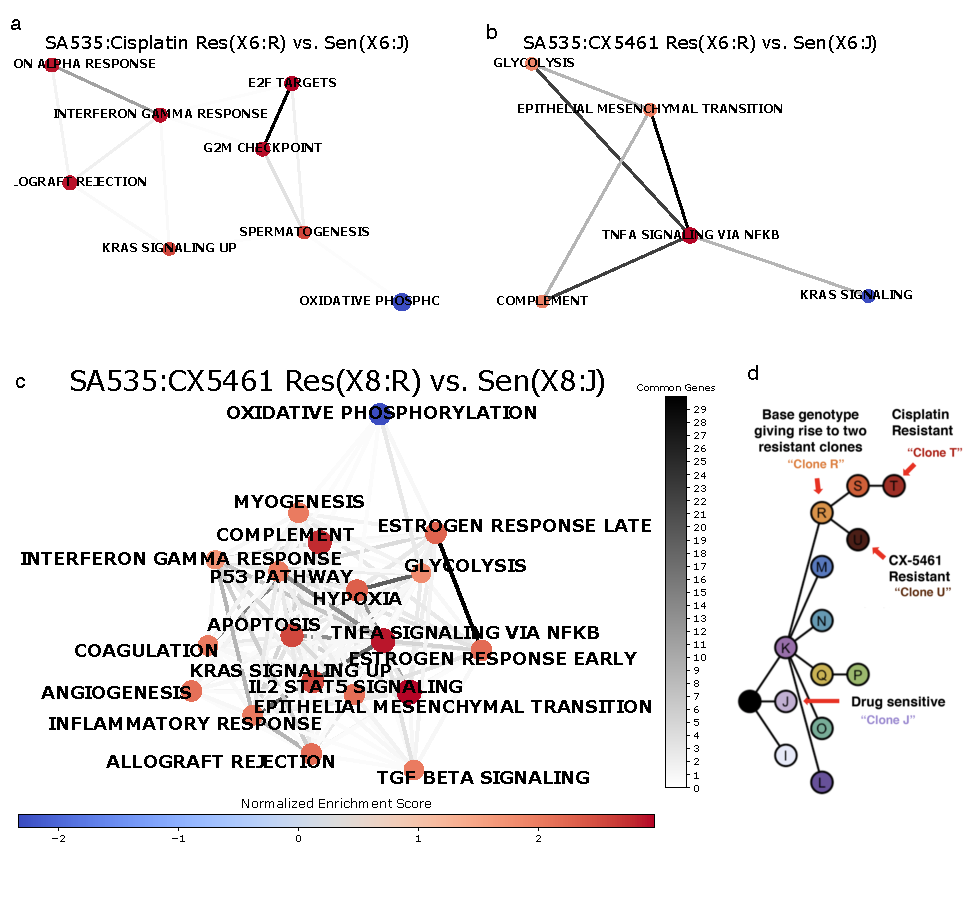
\includegraphics[width=\textwidth]{Figures/chap5/fig18_Rclone_pathways.pdf}
\caption[Pathway networks for the TNBC-SA535 precursor resistant clone.]
	{\small
	 \textbf{Pathway networks for the TNBC-SA535 precursor resistant clone R.} EMT is \textbf{Epithelial Mesenchymal Transition}, OXPHOS is \textbf{Oxidative Phosphorylation}. \textbf{(a)} Pathway network for SA535:Cisplatin comparing resistant clone R versus sensitive clone J at X6. \textbf{(b)} Pathway network for SA535:CX5461 comparing resistant clone R versus sensitive clone J at X6. \textbf{(c)} Pathway network for SA535:Cisplatin comparing resistant clone R versus sensitive clone J at X8. \textbf{(d)} Diagram of expected phylogenetic tree for SA535 taken from Chapter 4.
	 }

	\label{fig:Rpathways}
\end{figure}
%-----------------------------------------------------------------
In Chapter 4, I established that drug resistance could arise on a common clonal background for DNA damaging agents. Interestingly, the expression landscape of the common \textbf{precursor clone R}  showed upregulation  of \textbf{EMT, KRAS, TNFA signaling via NF-$\kappa$B and Apoptosis} \textbf{(\autoref{fig:Rpathways} a-d)}.

%combined phylogeny presented a \textbf{precursor clone R}, that gave rise to two distinct resistant clones \textbf{clone T and U}, respectively \textbf{(\autoref{fig:Rpathways} d)}. As above,  \textbf{clone R} pathways were also examined over time. Differentially expressed pathways between  \textbf{clone R} and untreated \textbf{clone J} was explored for both cisplatin and CX-5461 treated tumours in SA535. Predominantly showed upregulation  of \textbf{EMT, KRAS, TNFA signaling via NF-$\kappa$B and Apoptosis} \textbf{(\autoref{fig:Rpathways} a-d)}.

SA535 timeseries was treated with both cisplatin and CX-5461, and they shared many pathways that showed time dependent dynamics, such as \textbf{TNFA signaling via NF-$\kappa$B, Hypoxia, Apoptosis, UV response up, KRAS signaling up, Inflammatory response, Epithelial mesenchymal transition, TGF Beta signaling, Estrogen response} and \textbf{p53} pathways \textbf{(\autoref{fig:pathwaysnetworkcistrans} a} third, fourth column upper half and \textbf{\autoref{fig:networks} c, d)}. 
Notably, \textbf{clone R} showed many common pathways with two resistant clones but differed largely from untreated clone with high prevalence. Activated \textbf{interferon pathways} in SA535 cisplatin were only seen at early timepoints of \textbf{clone R} but not found in \textbf{clone ST} derived from this same precursor. There were fewer pre-treated   \textbf{clone R} cells with cisplatin.  


\section{Discussion}
In this chapter, I examined clone specific expression over time and treatments to establish how much of the transcriptome is potentially driven \textit{in cis}. I identified the key pathways and their temporal correlations involved in differential expression of resistant versus sensitive clones.

Because of the nature of the experimental design of timeseries longitudinal modeling, I was forced to collect tumour samples at different timepoints leading to the necessity of normalization and batch correction. 
However, I found that \texttt{SCTransform} for gene expression normalization and \texttt{edgeR} for differential expression was able to minimize batch effects. Nevertheless a small residual batch effect was notable via dimensional reduction with TNBC-SA1035 time series PDX. 
 

Copy number change \textit{in cis} expression accounts for $\sim${6.3\%-38.52\%} of clonal differences in resistant vs sensitive transcriptomes. The proportions of \textit{in trans} genes were higher as compared to \textit{in cis}, which reflects the degree of genomic instability overall and mirrors bulk analysis.
 
I observed that, as expected, the majority (3341 in total of DE genes) of \textit{in cis} gene expression changed reflected the direction of copy number difference between clones. However, a minority (777 in total of DE genes) showed counter expression implying some genes on CNA segments are regulated differently. 

\textbf{Here, I showed that CNA differences between clones can have a significant phenotypic effect on the transcriptome landscape.
I found over-enrichment of DE genes into specific pathways, including platinum resistance, showing that drug resistance phenotypes can be identified. } 


%I know that cis-regulatory mutations are skewed toward decreased expression while trans-regulatory mutations are skewed toward increased expression \cite{metzger2016contrasting}. 
 
%In breast cancer so far, many molecular pathways have been explicated while many others are either under investigation or to be investigated \cite{hanahan2011hallmarks}.
Trancriptional drug resistance for platinum has not typically been thought to have a genomic component but I quantified that some proportion of resistance was mediated by the changes in the genome, resulting a change in gene expression. The average CNA mediated platinum resistance accounted for 7.47\% maximum to 0.52\% minimum of the DE. 


Here, I found the top 5 cisplatin related commonly upregulated pathways in my data sets, including \textbf{TNFA signaling via NF-$\kappa$B, TGF  beta  signaling, Apoptosis, Hypoxia} and \textbf{Estrogen response} pathways. Moreover, \textbf{G2M checkpoint} and \textbf{E2F targets} were also highly activated and shared genes in 50\% of my datasets. 
\\
These pathways are already established to participate in platinum resistance but the granularity of the gene regulation in context of \textit{in cis} and \textit{in trans} has clinical implications for understanding mechanism of drug resistance. I showed that copy number differences between sensitive and resistant clones have a significant phenotypic effect on the landscape. 

Briefly, I found many known cisplatin resistance mechanism related genes, for example, \textbf{\textit{in cis}} regulated genes in my timeseries PDX  contain:
\\
MRP, COXC6  \textbf{(Pre-target mechanism of resistance)} \textbf{(see also \autoref{tab:pretargetcisplatinresistance})}.
\\
BAX, BCL2, BIRC5, CASP3, MAPK  \textbf{(Post-target mechanism of resistance)}.
\\
POLE, BRCA1, BRCA2, VDAC, MSH2 \textbf{(On-target mechanism of resistance)} \textbf{(see also \autoref{tab:ontarget})}.
\\
EGFR, HSP, TMEM, IDI \textbf{(Off-target mechanism of resistance)}.
 Many genes and pathways could be targeted at pre, on, post or off-targets of cisplatin resistance creating levels to circumvent drug resistance  \textbf{\autoref{fig:circumventingcisplatinresistance}}. However, \textit{in cis} genes may be less prone to variation, depending on the nature of the change. Complete deletion is irreversible, gene amplification could progress in either direction (more gains or loss after gain).
 Once the resistant clone having \textit{in cis} genes, becomes dominant and fixed, the possibility of clonal competition with less fit precursors no longer exists.

 %It could be possible that early in the course of treatment, the clone encoding the transcription mechanism got lost but only before its fixation.
 The genes that are controlled by CNA could be used as potential prognostic markers of treatment outcome.
\\
On the other hand, if the platinum resistance is not due to CNA genome, it may be more plastic over time. I also examined some of the \textit{in trans} mediated genes along with their drug holiday tumour expression and found many of those gene showed reversal of expression on drug withdrawl. For example, \textbf{MYC-(MYC-targets-V2 pathway)}  which is known to arise through multiple molecular mechanisms including gene amplification, gene translocation, enhanced transcription for other upstream pathways and decreased rates of ubiquitin-mediated proteolysis \cite{dang2012myc}. \textbf{MYC} is also under consideration as a potential therapeutic target for cancers expressing high levels of this oncoprotein \cite{reyes2015targeting}. It was found monotonically increasing with cisplatin treatment in SA609 along with reversal of expression on drug withdrawl, in drug holidays samples \textbf{(\autoref{fig:cistrans} a-right)}. 
\\
Other examples are from \textbf{(TNFA signalling via NF-$\kappa$B)}, which is another known pathway for cisplatin resistance and develops resistance through the activation of mediators, including anti-apoptotic genes and  \cite{godwin2013targeting}. \textit{in trans} genes, \textbf{EFNA and BTG1},  of \textbf{TNFA signalling via NF-$\kappa$B pathway} was also found to exhibit reversal of expression on drug withdrawl
 \textbf{(\autoref{fig:cistrans} c, d-right)}. 
 This kind of reversal is less likely to occur \textit{in cis} regulated genes, unless clonal proportions are changed.  


Other than the known cisplatin resistance pathways, I found \textbf{G2M checkpoint and interferons alpha and gamma pathways}, that were upregulated in resistant tumours. This was unique to SA1035 PDX tumour and may be a function of its \textbf{APOBEC} phenotypes. 
\\
Interferon pathways and G2M checkpoints, are not very well related to cisplatin resistance but early this year, a study showed that mitotic checkpoint could be targetable in overcoming platinum resistant TNBC \cite{ moens2021mitotic}. Furthermore, for activation of the interferon alpha signaling pathways, it has been shown that they could contribute to apoptosis and cellular senescence but are also attributed to increased migration and drug resistance depending on the interferon-stimulated genes transcribed \cite{provance2019deciphering, mojic2018dark}. New pathways require further validation. 
 
 I noticed that \textbf{TNBC-SA1035} PDX presented uniquely as compared to the other two PDX models based on the activated pathways and proportion of individual gene expression \textit{in cis} and \textit{in trans}. 
This could possibly be explained based on the initial heterogeneity of this tumour from Chapter 4. The DLP+ heatmap showed less heterogeneity as compared to SA609 and SA535 that were found to have more complex clonal structures. 
Also, SA1035 has APOBEC-HRD-like signatures with germline BRCA1 mutation unlike other TNBC, where, SA609 exhibits fold back inversion (FBI) signature and SA535 is BRCA 1 deficient tumour. 
\textbf{Upregulation of interferon pathways} in SA1035 PDX may be a consequence of its \textbf{APOBEC signatures}, where there is known mechanism of intrinsic immune response \cite{wang2018apobec3b}. Upregulation of interferon pathways are implicative of immunotherapy.


%\item  \textbf{\textit{BRCA1}} deficient TNBC-SA535 PDX exhibited activation of \textbf{IL-2\_STAT5 signaling} with cisplatin while \textbf{IL-6\_JAK\_STAT5 signaling} with CX-5461 in the same PDX. The potential addition of IL-6/JAK/STAT3 inhibitors with currently approved therapeutic agents directed against immune-checkpoint inhibitors are already under consideration \cite{johnson2018targeting}.

% \item I also summarized common genes that were found to be upregulated in all of 4 PDX series. Amid this list, I highlighted 4 interesting genes, out of which \textbf{\textit{ASPH}} monotonically increased with drug in our datasets, is catching attention in recent literature as a potential target in cancer therapy \cite{barboro2020aspartate, li2018expression, hou2018recent, kanwal2020aspartate}. Notably, \textbf{\textit{ASPH}} activates \textbf{Notch signaling} pathway and its upregulated expression stimulates the translocation of \textbf{Notch} to the nucleus consequently governing downstream target genes that mediate breast cancer cell adhesion and metastasis. Furthermore, these malignant phenotypes are reversed using a small molecule inhibitor (MO-I-1182) \cite{lin2019asph}.

 %\item Another aforementioned gene, \textbf{\textit{RAB10}}, belongs to the group of Ras-family proto-oncogenes and its knockdown has been linked to induce cell cycle arrest and apoptosis \cite{zhou2018down}, whereas \textbf{\textit{UBE3C}} and \textbf{\textit{YY1}} are known to be uniformly highly over-expressed in a wide range of human cancers.  Here I nominated them in the category of chemotherapy mediated increase in  differential expression in all of our time series \cite{pan2015ubiquitin, zhang2020ube3c, meliala2020biological, wan2012yin}. Interestingly, by observing drug holiday samples, I noticed that most of the expression in those tumour cells are reversed back toward untreated expression level, when the drug pressure is turned off.


\section{Limitations}

Although scRNA-seq has revolutionarized the field to detect large-scale transcriptional programs, it is unclear whether it accurately captures the behavior of individual genes. Hence, some validation would be required to confirm the results, such as, by using spatially resolved transcriptomics methods based on multiplexed single-molecule fluorescence in situ hybridization (smFISH). Also, immunohistochemistry (IHC) of tissue sections would support change in protein expression from untreated to treated tumours.

Since mRNA levels do not always correlate with functional protein levels, pairing single-cell RNA data with single-cell protein expression data is critical to making accurate and complete conclusions about cellular function.
For that purpose, imaging mass cytometry (IMC) would be able to validate scRNA-seq results.

I studied cisplatin in depth regarding its mechanism of resistance but for CX5461 resistance, more breast tumours would be required to make a generalizable conclusion. Also, more replicates would help overcome problem of low yield libraries.

%One limitation of this study was low number of cells in certain libraries. Another limitation could be the objective bias that comes from different collection time points. The serial passaging experiments were designed to stay in consistent with patient's tumour dynamics.




%Next I compared the emerging clone under drug pressure with the clone that could not survive the repeated drug exposures. I identified the following significantly up regulated pathways:
%- Apoptosis, Epithelial mesenchymal transition, Hypoxia, mitotic spindle, MTORC1 signaling, MYC targets-V1, P53 pathway, TGF Beta signaling, TNFA signalling via NF-$\kappa$B, UV response up, UV response down, KRAS signaling, Angiogenesis, PI3K AKT MTOR signaling, unfolded protein response.








